% Main document settings
%\documentclass[a4paper,11pt,twoside]{book}
\documentclass[a4paper,11pt]{report}

% Pacakages for Bibtex to work properly]
\usepackage[allcolors=blue,colorlinks=true]{hyperref}
\usepackage{natbib}
%%%%%%%%%%%%%%%%%%%%%
\usepackage[section]{placeins}

\usepackage{appendix}

%Making Landscape Pages
\usepackage{lscape}

% Page number Settings
\pagestyle{plain}
\usepackage{tabu}
% Set the text to 1.5 line spacing
\renewcommand{\baselinestretch}{1.5}

% Document Figure Settings
\usepackage{wrapfig}
\usepackage{pdfpages}
\usepackage[letterpaper, portrait, margin=1.5in]{geometry}
\usepackage{float}
\usepackage{graphicx} % Importing PDFs as Figures
\setlength{\belowcaptionskip}{-10pt}
\usepackage{rotating} % sideways figure


\usepackage[font=Large]{caption} % Chaning figure caption sizes

\usepackage[makeroom]{cancel} % Cancel math equations

% Make a custom list environment for no spacing between lists
\newenvironment{myitemize}
{ \begin{itemize}
		\setlength{\itemsep}{0pt}
		\setlength{\parskip}{0pt}
		\setlength{\parsep}{0pt}   }
	{ \end{itemize}         } 




% For Chemical Formulas
\usepackage{chemformula}

% For math equation in the Transcription area
\usepackage{amsmath}


% SI Unites
\usepackage{siunitx}
\usepackage{gensymb} %degree Symbol

% Inspiring Quote
\usepackage{epigraph}

% Bibliography preamble

%\renewcommand*{\nameyeardelim}{\addcomma\space} % Add a comma between author and year

%importing CSV Tables
\usepackage{csvsimple,booktabs,array,siunitx}
\usepackage{filecontents}

\captionsetup{
	font=footnotesize,
	justification=raggedright,
	singlelinecheck=false}

% Paragraph Spacing options
\setlength\parindent{0pt} % sets indent to zero
\setlength{\parskip}{10pt} % changes vertical space between paragraphs

% Custom Paragraph size just for the table of Contents
\usepackage{setspace}

% Customize Chapter Headings
\usepackage{titlesec} 


% Hyperlinks from Table of Contents
\usepackage{color}  %May be necessary if you want to color links
\usepackage{hyperref}
\hypersetup{
	colorlinks=true, %set true if you want colored links
	linktoc=all,   %set to all if you want both sections and subsections linked
	linkcolor=black, %choose some color if you want links to stand out
}

% Title Page Markup
\title{Identifying Biomarkers of Aging and Metabolic Disease through Multi-Omics Analysis of Heterogeneous BXD Mouse Populations}
\author{Author: Moaraj Hasan\\
	Direct Supervisor: Dr. Evan Graehl Williams, \\
	IMSB Supervisors: Dr. Prof. Ruedi Aebersold \& Dr. Nicola Zamboni \\
	D-BSSE Supervisors: Dr. Prof. Karsten Borgwardt }
\date{Sept 1st 2017, \\ Amended Nov 13th 2017}

\begin{document}
	
	\maketitle
	\let\cleardoublepage\clearpage
	
	% Inspirational Quote
	\chapter*{}
	
	\epigraph{“My earliest memories of my parents are of seeing my mother writing poetry and my father working diligently at his desk, happy and busy in their work. I did not know it then, but it is one of the most precious gifts a parent can give to their child”}{\textit{This thesis is dedicated to my parents Hasan Afzal and Aneela Anjum}}
	
	\let\cleardoublepage\clearpage
	
	% Re-render the table of content with the normal line spacing
	{\setstretch{0.5}
		\tableofcontents{}
	}
	
	\chapter*{Abstract} 

	A large-scale study of the BXD mouse genetic reference population metabolome, proteome, transcriptome, genome, and phenome was undertaken to determine factors involved in metabolic disease and aging. This investigation includes the use of statistical analyses to determine critical differences between metabolites, protein, and transcripts differentially expressing across diets and through the aging process in the mice. 
	
	To test the reproducibility of a metabolomics protocol used in previously published BXD mouse liver experiments a pilot study on 24 mouse livers was conducted. Additionally, the pilot study was used to optimize extraction parameters and determine whether all the homogenization and extracting steps were truly necessary. Once the procedure was optimized, 632 mice livers were subjected to metabolomics and analyzed. The mouse livers were also processed for proteomic and transcriptomics analysis using previously published protocols. As proteomics and transcriptomics sample require additional processing steps, a majority of these samples were not analyzed by the writing of this thesis.
	
	Many differentially enriched metabolites, protein, and transcripts between the diet and age cohorts were discovered and added to a list of biomarker candidates. Next pathway analysis was performed. Firstly, the steady-state metabolite data faithfully reproduced known concentration ratios in mice. Next, all the metabolites were plotted on their KEGG pathways and pathway in which we had high metabolic coverage and differences between age and diet cohorts was determined. Then a literature search was undertaken to determine a list of rate-limiting enzymes and metabolites in order to approximate the flux through certain pathways. The critical metabolites in the pathways were again appended to a growing list of possible aging and metabolic biomarkers. 

	QTL analysis found strongly regulated metabolites that had been previously identified and solved in a study with young BXD mice segregated in similar diet cohorts. The data from this experiment was used as a positive control for QTLs. Additionally, between diet fold changes of metabolites which were found in the previous study gave us a ground truth to benchmark our current sample preparation and metabolic analysis against. Additionally, three novel QTLs in central glucose metabolism, glutathione metabolism, and amino acid metabolism were found. Rudimentary analysis was performed on the proteomic and transcriptomic data as the datasets were largely incompletely at the writing of this thesis.

	Machine learning algorithms were used to determine the most important discriminating factors between diet and age cohorts. In the former case, a few metabolites with high bioavailability which were exclusively present in either the high fat or chow diet enabled a trivially easy determination of mouse diet. Training a classifier for age determination was not as easy using only the metabolites, however, some metabolites such as non-fully oxidized fats proved useful in discriminating between the young and old mice. This corroborates prior knowledge in which oxidation efficiency decreases as mice age. This analysis was also performed for the proteomic data as using fold change analysis between the proteomes of young and old mice did not yield many hits.

	From this analysis, a list of candidate genes and proteins that regulate these metabolites is made and a proof-of-concept integrated analysis is done in Linoleic acid and Tyrosine metabolism. For those pathways that have knock-out mice available or downstream enzymes, inhibitors are added to a list of metabolites to follow up with in validation experiments due to occur at the beginning of next year.
	
	\chapter{Introduction}
	
	The world post-industrial revolution, once riddled with infectious disease and appalling living conditions brought on by the influx of rural peoples into the poorly equipped cities caused a striking number of deaths from conditions that rarely occur in modern life\citep{JOEPINSKER2013}. The tremendous progress in health outcomes today can be attributed to the sanitary revolution; the successful implementation of health efforts such as large-scale water sanitation and sewage disposal and scientific efforts such as the increase in our understanding of germ theory, the development of antibiotics and vaccines \citep{Mackenbach2007}. Although we are protected from many conditions that would be fatal in the past, the result of living longer and having caloric surpluses in our diets has led to the manifestation of my other chronic conditions. As a result, the focus of biomedical research has shifted from infectious disease to diseases like cancer which are age-related degeneration is a risk factor and metabolic disorders which are associated with poor diet and sedentary lifestyles. 
	
	Despite large efforts using model organisms, there are mabny shortcomings in the understanding of the pathways and molecules involved in the onset and progression of chronic diseases. How these pathways interact with aging also remains unclear to due to the financial and logistical challenge of large longitudinal studies in vertebrates \citep{Williams2015TheAnalysis}. Additionally, there is a large difference in the chain of translatability between chronic illnesses challenging the biomedical research community today, and the infectious diseases that are more tractable to find cures for. In diseases like bacterial infections, \textit{in vitro} mechanistic insights and efficacy of anti-biotic activity translates well from \textit{in vitro} into in vivo models\citep{Moffat2017a}. For example, antibiotics with strong plate clearing capacity in Petri dishes have a high chance of killing the bacteria in human tissue barring safety and bioavailability concerns. The chain of translatability is much weaker for a complex disease like age related reduction of hepatic functions which can be caused by mutation accumulated through the aging process and are more difficult to mechanistically study in \textit{in vitro} models \citep{Moffat2017a}. To address this issue, the use of multiple model organisms studied in different cohorts of diet, genetic background, sex and age over the lifetime of an organism can be used to deconvolute the mechanistic roles these factors and allow us to screen interventions that could be translated to longer healthier lifespans in humans \citep{Armanios2015}. The goal of the intervention is not simply to extend lifespan but to maintain the organ systems and cognitive faculties of a person as there in their youth, into old age \citep{Armanios2015}.
	
	\section{Project Outline}
	
	\begin{figure}[htb!]
		\makebox[\textwidth][c]{
		\includegraphics[width=1.2\linewidth]{1.Introduction_Figures/Experiment_Process.pdf}}
		\caption{The time line of the BXD aging mouse population study. Over 2000 mouse in 83 strains are segregated into two diets and aging for eight, twelve, sixteen and twenty months. During their lifetimes all the mice are subjected to a range of phenotype examinations. Only the mice that make it to the exact time mark (ie. 4 months) are sacrificed. The  mice are euthanized using a strong anesthetic and have all 26 organs harvested in a timely manner to reduce the post mortem changes in the physiology. In this study, only the frozen livers are pulverized and processing for transcriptomics, proteomics and metabolomics studies.}
		\label{fig: Outline of the BXD Aging Population Study}
	\end{figure}
	
    The design of this study is to have a large group of inbred mice segregated into two diet groups and sacrificed in four age cohorts of 8, 12, 16 and 20 months. This allows us to interpret the genetically driven factors that change between the aging and control for the environmental input (diet). This study is a follow up to a study by \citet{Williams2016SystemsFunction} in which important regulators of the electron transport chain respiration and cholesterol synthesis were found. All of the mice in the study are the progeny of two founder strains and show genetic differences at 5 million loci. As the mice are kept in the same housing environment, allowed to eat and exercise \textit{Ad libitum}, the study is designed to uncover gene interaction with age and diet that would otherwise be confounded by environmental variables. An assumption in the study is that mice from the same strain are considered biologically identical despite the stochastic nature of the expression of certain traits\citep{Czyz2012Geneticdifferences}.
    
    At the beginning of this masters thesis, all the mice had been phenotyped, sacrificed with their liver extracted and ready for processing for the various omics analysis. Of the over 2000 mice that were enrolled in the study, 621 mice survived to their sacrifice date ensuring there at least 2 biological replicates in every age and diet cohort which are subjected to metabolomics, proteomics and transcriptomics analysis. Significantly enriched metabolites, proteins, and transcripts were all found. Metabolite QTLs found in previous studies were detected alongside two novel QTLs. Network analysis indicated many significantly enriched pathways, with respect to diet and age. Although the metabolomics analyses were completed for all the mice, proteomics and transcriptomics data are incomplete, and the findings in this thesis are subject to change as new data are introduced. Machine learning techniques were used to determine age-related proteins, in a data set where it was difficult to discern between mice of different age cohorts with simply using fold changes. It was thought, the use of an ensemble of proteins, similar to the increase in power of using a haplotype rather than specific SNPs, would give us higher discrimination power between the age cohorts\citep{Lorenz2010Performancebarley}. For transcript data, the highly expressed genes were plotted alongside proteins on integrated maps in order to determine causal graphs for specific metabolites.
	
	\section{Gene-Function Paradigms}
	
	\begin{figure}[ht]
		\centering
		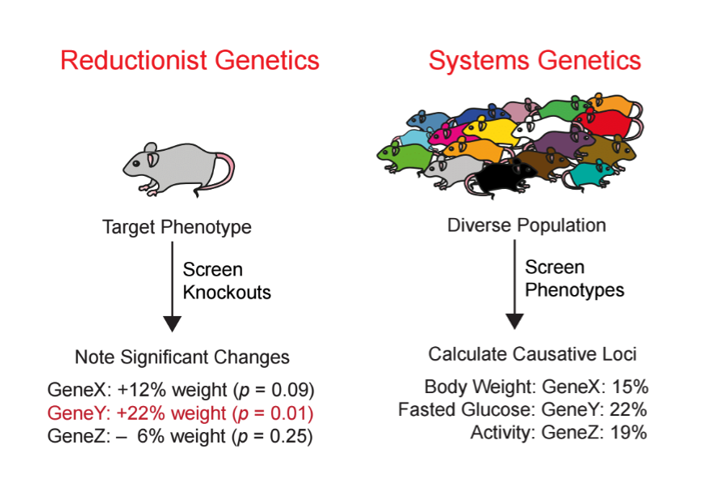
\includegraphics[width=\linewidth]{1.Introduction_Figures/Reductionnist_genetics.PNG}
		\label{Reductionist vs. Systems Genetics}
		\caption{Adapted with permission from \citep{Williams2014Thesis}. An illustrated example of the two school of thought concerning the regulation of body weight by a single loci. \textbf{Left} In the case of reductionist genetics, genes are targeted by knock-down experiments to determine if any have a significant effect on the target phenotypes (body weight). This is done with the assumption that there is a strong direct link between the loci's expression and the phenotype.\textbf{Right} In the case of systems genetics, it is assume that genetic variants contribute small effect sizes which are pooled to determine the final phenotype. In the systems approach, natural or inbred genetically heterogeneous populations are screened in a consortium of molecular factors which can explain the variation of the phenotype in the population.}
	\end{figure}
	
	The reductionist approach to genetics involves identifying a gene of interest and altering it through means of random or directed mutagenesis, followed by observing the manifested effect of the gene's absence or super over-expression \citep{Williams2015TheAnalysis}. In reverse genetics, a diverse panel of animals is used and phenotypes variants are probed at the genetic, proteomic, and metabolic levels to determine the sources of the varied physical characteristic. In reductive study design, when a gene is knocked-out or augmented to show a 10-fold greater expression than the normal physiological range, the intervention is not addressing the question of what the physiological function, but rather illustrates the outcome of large changes in the physiology that are either fatal or rare in real biological systems. Moreover, reductive study design usually observe the effect of interventions on a single  loci and are not highly instructive for complex diseases like diabetes \citep{Williams2015TheAnalysis}.
	
	In contrast, forward genetics involves determining polymorphisms that modulate certain phenotypes and disease risks. This is the generalization of medial inheritance analysis applied to complex traits \citep{Williams2015TheAnalysis}. Certain genes are altered through direct editing, silencing or mutagenesis with the commensurate phenotype used to induct the function of the gene. 
	
	As age-related degeneration is a multi-factorial and highly complex disease, systems genetics paradigm is used in this study. Many genes, proteins and metabolites may be differentially expressed as mice age, finding a genetic link between many factors that have large variances between strains in different ages can allow us to identify biomolecules that arise from age-related degeneration.
		
	\section{Reverse and Forward genetics}
	
	There are two different study designs that can be used to determine the function of a gene as shown in figure \ref{fig:Forward and Reverse Genetics}. With a reverse genetics design, a specific gene is disrupted usually through a knockout or by inserting a viral promoter that causes the super over-expression of genes to determine the down-stream effects. The disruption of the gene can be done in a targeted manner using siRNA, CRISPR-Cas9 or homologous recombination or can be done in a non-targeted manner such chemical or transposon-mediated mutagenesis followed by screening the library of individuals\citep{MelindaB.TierneyandKurtH.Lamour2005}. For smaller organisms such as  \textit{C. elegans} or \textit{D. melanogaster}, random mutagenesis is a tenable strategy, however, for larger more complex organism targeted techniques are preferred \citep{MelindaB.TierneyandKurtH.Lamour2005}.
		
    \begin{figure}[!htb]
	\centering
	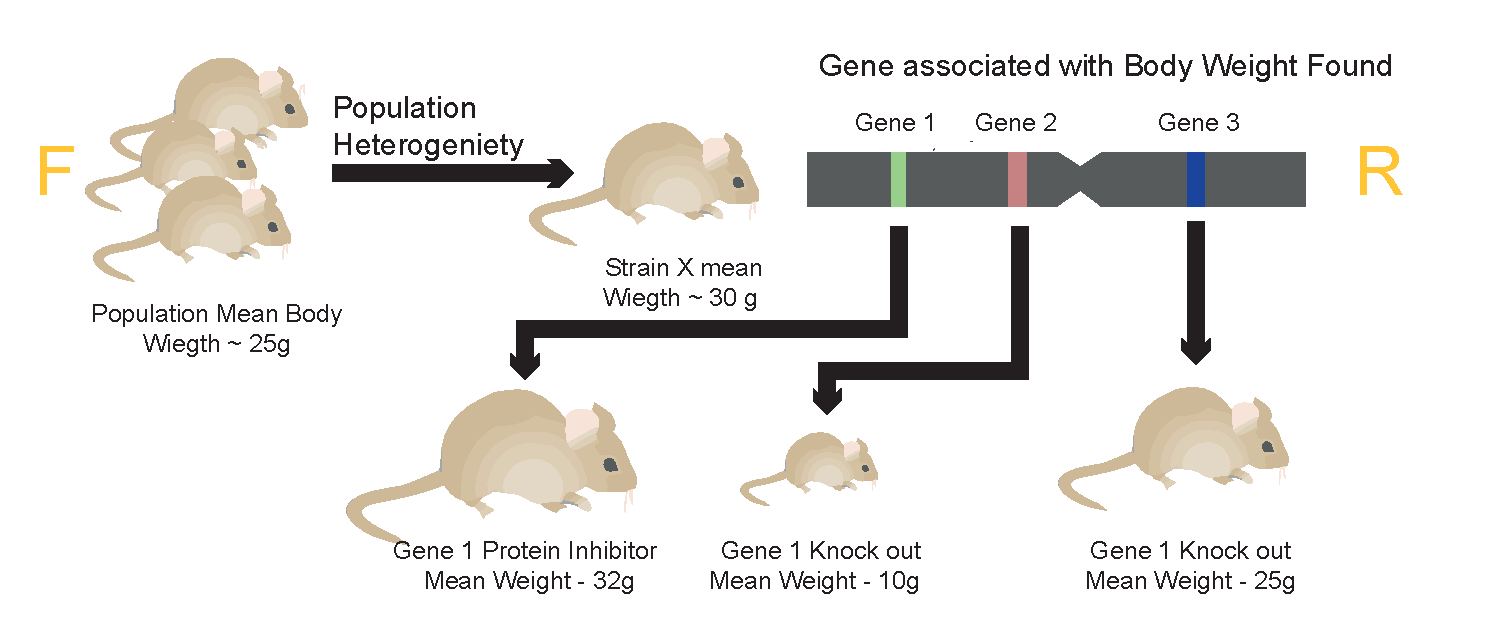
\includegraphics[width=\linewidth]{1.Introduction_Figures/Forward_Genetics.pdf}
	\caption{Summary of forward and reverse genetics experiments which can be used to determine the genetic drivers of a phenotype.\textbf{Top:} Schematic of the reverse genetics approach. \textbf{Middle:} Schematic of the forward genetics approach\textbf{Bottom:} Combination of both study types in which forward genetics techniques are used to find candidate loci that may regulate a phenotype, and reverse genetic techniques to validate these hypotheses.}
	\label{fig:Forward and Reverse Genetics}
	\end{figure}
	
    Forward genetics refers to an experimental design where studies are initiated to determine the genetic underpinnings of observable phenotype variation between a heterogeneous population of an organism. Variants that deviate from the average trait presentation in heterogeneous population can be measured as physiological traits such as body weight and morphology to molecular variation or protein profiles, transcript abundance and DNA sequence variants \citep{MelindaB.TierneyandKurtH.Lamour2005}. In the case of genetic reference populations such as the BXD mice, there is a limit to the variation that comes from the allele differences in the parental strain \citep{Williams2017ResourcesGenetics}. Additional trait variation is introduced through controlled out breeding with members of wild populations\citep{MelindaB.TierneyandKurtH.Lamour2005}.
	
	 The widespread availability of sequence data gives us many advantages, previous researchers did not have. Once individuals in populations with traits of interest are identified, having access to all gene sequences for the organism allows us to determine a list of candidate loci that influence the phenotype of intrest and thier interaction with age, sex and diet. Once there is a finalized list of hypothesized genes through to be driving aphenotype of intrest, the exact function of the list of these genes is elucidating using reverse genetics techniques\citep{MelindaB.TierneyandKurtH.Lamour2005}. For example, some BXD mice strains exhibit high body weight despite being on a lean chow diet, genes that show hyper or hypo-expression can be or modified in a batch of mice in a follow up experiment to measure their effect on the phenotype (Figure \ref{fig:Forward and Reverse Genetics} Bottom).

	
	\section{Systems Approach to Complex Trait Analysis}
	
    In this study the use of multiple biomolecule readouts for every mouse allows us to take a Systems Genetics approach to complex trait analysis. Systems Genetics is an approach that tries to understand the communication between of multiple layers of biological information and determine how the sum of their contributions results in the presentation of a complex trait \citep{Civelek2014SystemsTraits}. A systems approach requires many experimental techniques to oberserve and collect data on a range of phenotypes and statistical methods to quantify and organize these molecular phenotypes like proteomes, transcriptomes, and genomes into interacting circuits with common inputs and phenotypic outputs\citep{Civelek2014SystemsTraits}. The output which is the oberserved phenotype is thus generated by multiple functional molecules in the cellular milieu on the level of genes, transcripts, proteins, metabolites, and their interactions within themselves \citep{Civelek2014SystemsTraits}. Additional inputs from an organism's environment are manifested at the cellular level through changes in chemical concentrations and signaling states around cells. These environmental factors also interact with all the aforementioned molecules within a cell in complex ways \citep{Civelek2014SystemsTraits}. Figure \ref{Multi-Layer Trait Determination} illustrates the complicated reciprocal nature of the interaction between genes, transcripts, metabolites and metagenomes that may lead to a specific phenotype presentation. 
	
	\begin{figure}[htb]
		\centering
		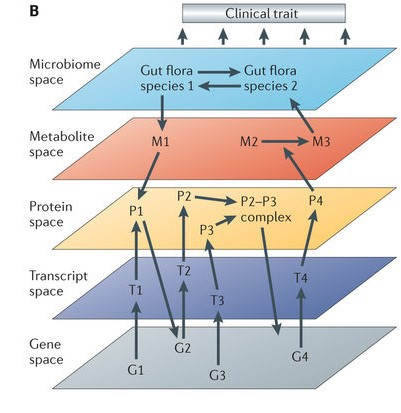
\includegraphics[width=0.6\linewidth]{1.Introduction_Figures/nrg3575-f1.jpg}
		\caption{Taken from \citeauthor{Civelek2014SystemsTraits}, this figure illustrates the complex determination of a clinical by multiple interacting layers. The gene, transcript layers reciprocally interact with proteins in an or organism that bias the metabolome and increase the production of a metabolite. This metabolite causes changes in the microbiome that propagates an effect back down to the genetic level, illustrating the complex causal structures that produce a single observable trait.}
		\label{Multi-Layer Trait Determination}
	\end{figure}
	
    Unlike Mendelian traits, a concerted constellation of changes sum to generate a complex trait. Therefore, finding mechanisms for complex trait presentation are difficult to determine from a single layer of molecular information. Instead, there is a requirement to understand the pathways and networks that underly traits which can be symptoms of a metabolic and age-related disease. A node in these networks has a small contribution to the overall phenotype and may have stochastic components to its manifestation. As a result, the complete mechanistic decomposition of complex traits remains challenging even with large amounts of molecular data available on humans and model organism \citep{Civelek2014SystemsTraits}. 
	
	With vast amount of molecular data available to the public, it is often just as important to know which complex traits are tractable for genetic analysis. A key criteria to identifying whether the causal mechanism of a trait can be determined is if the trait shows a level of heritablity in the test population.
	
	
	\section{Heritability}
	
	A fundamental question in biology is whether a presenting trait is inherited from parents or the result of environmental factors. The Heritablity $(H^2)$ is an attempt to quantify the relationship between genetics and the environment in the determination of a complex trait phenotype \citep{Visscher2008Heritabilitymisconceptions}. In order to calculate heritability, it is assumed the phenotype measured is determined by a combination of environmental and genetic factors. 

	\begin{equation} \label{eq1}
	Phenotype (P) = Genotype (G) + Environment (E) 
	\end{equation}

	All of the variation that is observed in the trait is thus the sum of variation in genetic and environmental factors  \citep{Visscher2008Heritabilitymisconceptions}.

	\begin{equation} \label{eq2}
	 \sigma_P^2 = \sigma_G^2 + \sigma_E^2
	\end{equation}
		
    The genetic variance in the formula can be partitioned into additive breeding or strain-related effects, effects of the dominance, and effects of epistatic interactions \citep{Visscher2008Heritabilitymisconceptions}. The narrow sense of the concept $h^2$ quantifies the portion of variation within an observed population that can be explained by only breeding value differences, as opposed to the broad sense values $H^2$ used in this which includes dominance and epistatic interactions and is defined below\citep{Griffiths1999}.
	
\begin{equation} \label{eq3}
H^2 = \dfrac{\sigma_G^2}{\sigma_P^2} 
\end{equation}
	

    $H^2$ ranges from [ 0.0 , 1.0 ], with the low heritability meaning there is a low probability phenotypes in an offspring with a specific genotype will show a particular phenotype, and high heritability values [ 0.7, 1.0 ] stating, the phenotype observed in the offspring will be similar to parents with the same allele.  
	
    In order to determine heritability, an ideal experiment involves creating an environment that is identical in every aspect for a particular population of organisms\citep{Griffiths1999}. As the population grows and develops, differences that manifest in different traits can be observed . In a well-controlled experimental study, the population is subject to the identical environmental conditions and unless the individuals in the population are genetically identical observed differences can be attributed to genetics\citep{Griffiths1999}. A constant environment is not necessary for heredity calculations if all the variations in the environments are known and can be controlled for. Thus determining the heritability of a metabolite, protein, and transcript allows us to estimate which traits have a high likelihood of segmenting between populations according to their genotype resulting in strong QTLs. Conversely, if we do not see a strong QTL where we should, a heritability measurement before and after controlling for environmental factors, if significantly higher can reveal why a strong QTL is not observed.
	
\subsection*{Caveats of Heritability Calculations}
	
	In this framework for studying heritability, if either there is no variation in the genotypes, theoretically there can be no variation in the phenotypes due to genes and heritability is zero. However, even in mono-zygotic twins or inbred mice of the exact same genotype and rearing, slight variations in physical features can be seen. There are stochastic manifestation of environment factors, especially over a long life time that can lead to the divergance of a physical trait\citep{Czyz2012Geneticdifferences}. For example, in a pair of twins that both smoke, cancer risk does not increase in a discrete, constant level with every cigarette smoked. The incipient metastatic event occurs through random interactions between the polyaromatic hydrocarbons from the smoke and the replication machinery in the nucleus of a lung cells. One hydrocarbon may cause a critical p53 mutation by chance in one twin leading to cancer while the other twin might smoke more yet remain healthy.
	
    Illustrated in the example with BXD mice in the following section, heredity is difficult to deduce without environmental controls. The lack of conditional controls make studies of complex traits and their heritability in humans significantly complicated. As such, complex trait analysis in mammals are most frequently performed using a recombinant inbred population of mice \citep{Williams2015TheAnalysis}, as is done in this project. When outbred and wild strains are used, additional complicating factors for the experimental design need to be considered and the studies have lower statistical power for the same number of mice. Additionally, heritability is hard to measure robustly for behavioral and complex traits such as intelligence but is strongly predictive in core physiological traits across large phylogenetic distances \citep{Falconer1996IntroductionGenetics}. Thus highly heritable core physiological traits we may discover in mice also have a good chance of being heritable in humans.
	
	\section{Studying Heredity in Model Organism Populations}
	\begin{figure}[!htbp]
		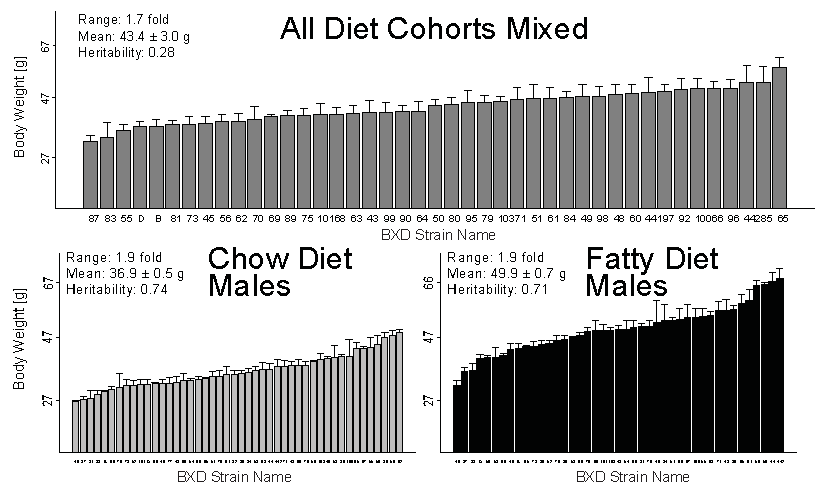
\includegraphics[width=\textwidth]{1.Introduction_Figures/BodyWeights.pdf}
		\caption{ \textbf{Top:} Average body weight of BXD mouse strains in a mixed cohort of CD and HF mice. \textbf{Bottom:} Average body weight of BXD mouse strain in CD cohorts and HF cohorts separately
			Heritability of Body Weight and fixed and mixed Diet population}
		\label{fig:Heritablity in Diet and Mixed Populations}
	\end{figure}
	
	For consideration, BXD mouse weight which is higly heritable has an observed heritability of 0.74. This shows that while the nutritional intake of the mice, which is the only evironemntal factor, changing between the animals, has an effect on body weight, a major portion of  the variation in the mouse body edihts can be explained by genetics \citep{GerhardAdam2012}. An important distinciton is that hertibality explains the between mouse variance in a specifc mouse population but does not actually provide any mechanistic insights into the apidpose tissue anabolism or fatty acid metbolism that may explain the combintioan of alleles that could predict a particular weight range for a mouse having a certain haplotype \citep{GerhardAdam2012}.
	
     In figure \ref{fig:Heritablity in Diet and Mixed Populations} the panel across the top shows the body weight of mice from CD and HF mice mixed in a single population. There is a mean body weight of 43.4g and a 1.7 fold difference between the lowest body weight mouse strain, BXD 87, and the highest, BXD 65. The diets have not been adequately controlled for in the mixed population so heritability is only 0.28. Here, diet plays a larger role in the observed heritability of body weight, as it is not as tightly controlled as in the previous example, where all animals were fed the same diet. When mice have different diets, as here, we see that genetic background only influences 28\% of the variation between individuals' body weights, while the remaining 72\% is related to dietary differences or other non-controlled environmental variants \citep{GerhardAdam2012}.  
     
     The panels across the bottom of figure \ref{fig:Heritablity in Diet and Mixed Populations} show the body weights of mice segregated into CD and HF in separate cohorts. When the mouse population is segregated there is a large difference in the environment the mice a reared in but within the diet groups, the environmental conditions (dietary intake) is constant. However, the genetic variation between the mouse strains within each of the diet cohorts still remains \citep{GerhardAdam2012}. As a result, a heritability of 71\% and 74\% is calculated for the CD and HF cohorts respectively because the variation of the mouse body weight in each diet cohort can be mostly attributed to genetics. 
	
    This is why model organism populations are used for complex trait analysis in this study. The inbred stocks are invaluable to the study of genetic drivers because of the amount of genetical diversity and environmental factors can be controlled. This is also the reason complex trait analysis is so difficult in human and wild populations. The number of lifestyle decisions a human can make to change their environmental context is much larger than that of most wild populations. On top of this, humans and mice have several additional layers of redundancy and regulation in their biology as compared to simpler organisms like fruit flies\citep{Kafri2006Thecircuits}. If one was to compound the effect of mixed diets, family and a myriad of unknown contributing factors on top of this biological redundancy, finding QTLs and genetic drivers for phenotypes becomes quite difficult. 
	
	\section{What is QTL Analysis?}
	
	Quantitative Trait Locus (QTL) analysis is a statistical method which permits determining the probabilty of linkage between DNA sequence variance with observed phenotypic variants \citep{Falconer1996IntroductionGenetics}. In order to perform QTL analysis, populations of individuals that vary in the trait of interest are required \citep{Mackay2009TheProspects}. In figure \ref{fig:QTL Explanation} the distribution of a phenotype parental strain along side genotype are shown. Through successive recombination events in the F2 and recombinant inbred(RI) mice, the population phenotype converges to an average of the parental phenotype in most traits. 
	
	\begin{figure}[ht!]
		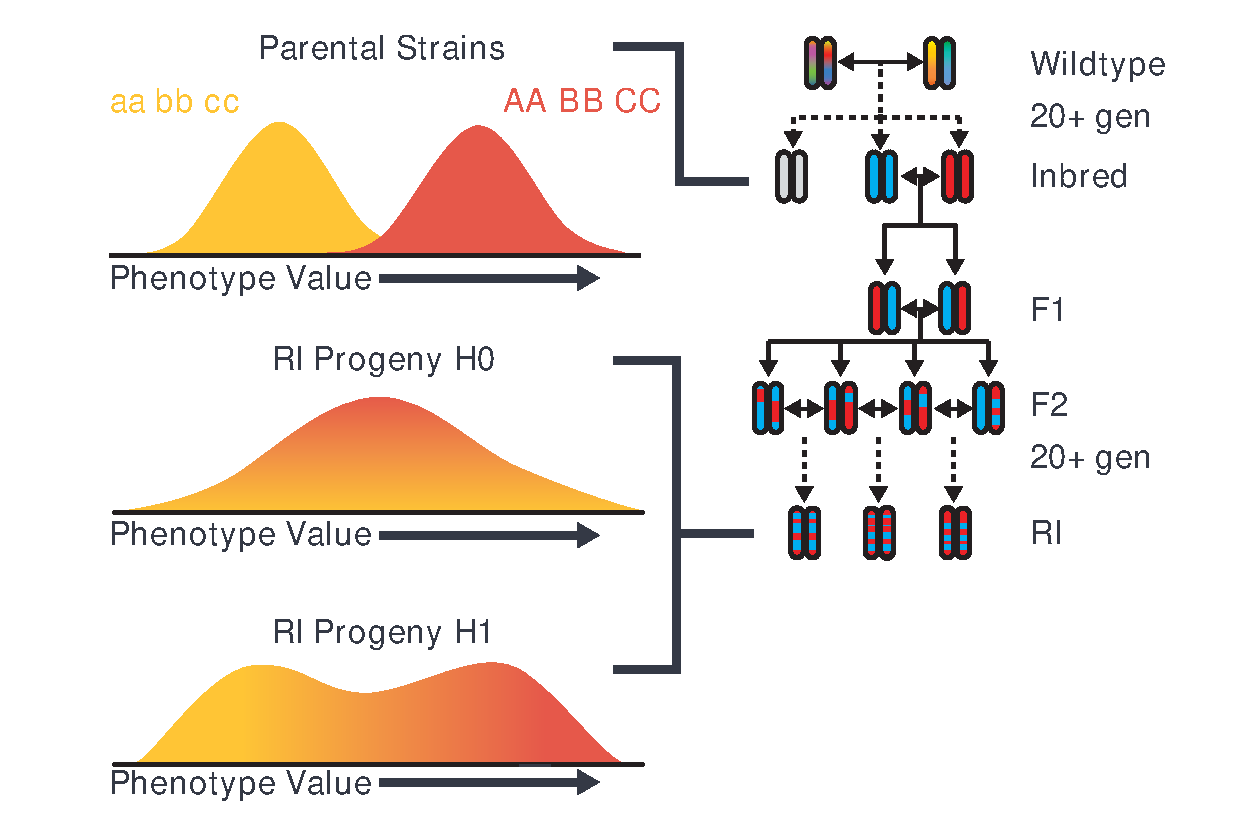
\includegraphics[width=\linewidth]{QTL_Results/QTL_Introduction.pdf}
		\caption{Adapted from \citep{Williams2017ResourcesGenetics} This figure shows the principles of QTL mapping in an inbred population derived from two parents. Distinct phenotypic trains in the parent's strains combine to form a continuum of the traits in the recombinant inbred progeny. The purpose of QTL mapping is to determine which of the inherited markers explain the variance in the trait}
		\label{fig:QTL Explanation}
	\end{figure}
	
    Depending on how many loci determine a trait, a range of values can be seen in the continuous trait in offspring that have different combinations of the parental alleles. In this case (shown in figure \ref{fig:QTL Explanation} H0), If there is no effect from certain loci, there will be no differences in the trait with respect to the genetic background of the mice. If a locus regulates a quantitative trait, then one would see two populations of mice when all of the strains are ranked with respect to the trait and a bimodal distribution emerges (figure \ref{fig:QTL Explanation}, H1). Strains with one of the parent's alleles in that position and one with high values for the trait with the other parental loci\citep{Mackay2009TheProspects}. As one performs this test for a single trait across the entire genome, loci that segregate the strains into two populations are thought to regulate the trait. In the BXD mice, all of the strains have been sequenced and each of the marker blocks has annotated with the parental origins \citep{Mulligan2017GeneNetworkGenetics}.  To perform QTL analysis on the BXD mice, a quantitative mapping is done with a trait against an array of molecular markers at approximately 3Mb marker intervals. 
	
	In order to perform a QTL screen one tries to determine the parameters of the following relationship:
	$$P_i = f(g_i) + e_i $$
	Where $P_i$ is the individual's phenotype
	$g_i$ is the genotypes and $e_i$ is an environmental contribution.
	Moreover, is is assume that covariance of genotype and environment are 0 \citep{Broman2009AR/qtl}
	$$ \sigma_{phenotype}^2 = \sigma_{genotype}^2 + \sigma_{envir}^2 + \cancelto{0}{2{\sigma_{G x E}^2}} $$
	
	An appropriate additive model for mapping phenotype to genotype is described as such:
	$$ f_a(g_i) = \sum_{j \in QTL }\beta_jg_{ij} + \beta_0 $$
	where $g_{ij}$ is marker j for individual i with genotypes values \{0,1\} 
	
    There is another assumption that typically if an offspring is getting half of their genes from the mother, and the other half from the father that the expected phenotype they will display is an average between the parental phenotypes \citep{Broman2009AR/qtl}.
	
	$$ E[f_a(g_i)] = \dfrac{f_a(p_{parent-1})}{2} + \dfrac{f_a(parent-2)}{2}$$
	
    A test is performed at each marker site to determine whether the phenotypes of individuals that vary at the marker in genotype $g_{ij}$ present phenotypes that also exist in two distinct populations with $\mu_0$ and $\mu_1$ akin to the parental distributions in figure \ref{fig:QTL Explanation}. In order words, if there is a change in genotype at loci but no commensurate change in the phenotypes of indivudials with distint genotypes at the loci, there will be a low probability the trait is regulated by elements in the area\citep{Broman2009AR/qtl}.
	
	$$LOD = log10\prod_{i=1}^{N}\dfrac{P(p_i| g_{ij},\mu_0,\mu_1,\sigma )}{P(p_i|\mu,\sigma) } $$
	
    In order to reduce the multiple testing burdens of testing 1000s of genetic markers against a single phenotypic trait, we can try to compute the null distribution of the LOD scores rate by randomly permuting the genotypes 1000-10000 times and recomputing the LOD scores. For every marker, we can directly determine the determine the LOD score threshold above which there is only a 0.05\% chance of a LOD score by chance  \citep{Broman2009AR/qtl}. Once a strong QTL is discovered and the gene within the QTL region may be related to the phenotype, a congenic strain of with the complete set of alleles from a single parent strain, except for at this one loci mice is produced as a validation.
	
	\section{QTL vs. GWAS}
	\label{sec:QTL vs. GWAS}
	
	QTL mapping and Genome-Wide Association Studies (GWAS) both attempt to determine relationships between genotypes and observed phenotypes. QTL mapping identifies regions of a genome that co-segregate with a treat in an F2 or recombinant inbred population. Using this techniques the key components of the cholesterol metabolism pathway in BXD mice have been dissected in the previous iteration of this study \citep{Williams2016SystemsFunction}. 
	
	Despite this success, QTL mapping has limitations in the number of alleles that can be assayed at once and mapping resolution. When using QTL mapping in a recombinant inbred population, the total diversity of alleles which can be assayed is limited to only those alleles present in the founder strains. Moroever, if the founder strains have the same genotype in a region of the genome, it cannot be used for QTL mapping. Additionally, the resolution of the mapping is limited to the sizes of recombination blocks on the chromosomes\citep{Korte2013Thereview}. These can be reduced through extensive crossing but long lengths of the chromosome which have low recombination frequency are mapped as large QTLs containing many genes making it difficult to find causal genes for a trait within the QTL \citep{Korte2013Thereview}. A solution to the first issue was proposed by the collaborative cross(CC) consortium in which 6 different stains of \textit{Mus musculus}, \textit{Mus domesticus} and 2 from other sub species of mice were crossed in order to produce a mouse stock with significantly higher genetic marker densities. \citep{CollaborativeCrossConsortium2012ThePopulation.}. The some of the CC mice strains however have too much genetic distance between eachother which has led to problems breeding the mice.
	
	GWAS overcome the resolution limits of QTL analysis by using higher density markers such as SNPs instead of recombination intervals but run into multiple testing issue. Similar to QTL mapping, GWA studies test the association between a particular trait and a genetic marker across a large population of individuals. GWAS and QTL mapping provide hypothesis discovery and serve as the basis for further direction knock-out or mutation experiments to validate a genes function. 
	
	\section{RI Mouse Population for GxE}
	
	Quantitative phenotypes are partially determined by $GxE$ interactions. $GxE$ interaction are the changes in a phenotypes as a result of the interplay between genetics with diet, age, differences in social interaction and exposure environmental stressors like heat, drugs, and pathogens \citep{Williams2017ResourcesGenetics}. To accurately elucidate $GxE$ in the context of QTL mapping, mice, and other isogenic model organisms are often used because a researcher can readily purchase or generate large cohorts of animals with similar genetic backgrounds and can impose well-controlled perturbation across these cohorts\citep{Williams2017ResourcesGenetics}. This enables the evaluation of complex environemental effects  with good power that would not be possible in wild animal or human populations \citep{Williams2017ResourcesGenetics}. 
	
    As discussed in section \ref{sec:QTL vs. GWAS}, one disadvantage for RI strains is that they are difficult and time-consuming to produce, and as they serve as a fixed reference population, they cannot comprise all possible polymorphisms across a species \citep{Williams2017ResourcesGenetics}. For instance, the large BXD population contains approximately 5 million sequence variants across its strains \citep{Andreux2012SystemsTraits}. As the BXDs are generated from two independently-derived inbred strains—of the many dozens of independently-derived inbred strains commonly available from providers like The Jackson Laboratory. These two strains contain ~44\% of all sequence variants which occur across the most commonly used laboratory mouse strains; thus more than half of all common laboratory variants will not be represented in a study using the BXD population \citep{Williams2017ResourcesGenetics}. Despite this low coverage of the total polymorphism space in mice, a study using 150 stains of BXDs, a cohort of mice containing over 12000 potentially harmful missense mutations  yielded a wealth of disease-relevant insights by performeing QTL mapping on thousands of phenotypes\citep*{Wang2016JointRisk}. This study not only shows the power of using this refrence population to determine regulatory sites for disease relavent phenotypes but is also a rich dataset to test hypotheses against. Eventhough the BXD mice are crossed for over 20 generateions, some stretches of the RI mice genome will be almost completely identical by descent \citep{Wang2016JointRisk}. These chromosomal regions are known as blind spots for QTL mapping as they should not contribute to trait variance\citep{Wang2016JointRisk}. In any given genetic interval, the collaborative cross mice, have much higher marker densities and smaller recombination blocks as compared to the BXD mice which have a sixfold lower polymorphism load. If a phenotype maps to an area in both CC and BXD mice, it is relatively simpler to determine the driving gene in the BXD as there is reduced the number of viable candidate genes in a QTL one has to consider \citep{Williams2017ResourcesGenetics}.
	
	\section{Study Design}
	
	\subsection{Model Mouse Population: BXD Mice}
	
	\begin{figure}
		\centering
		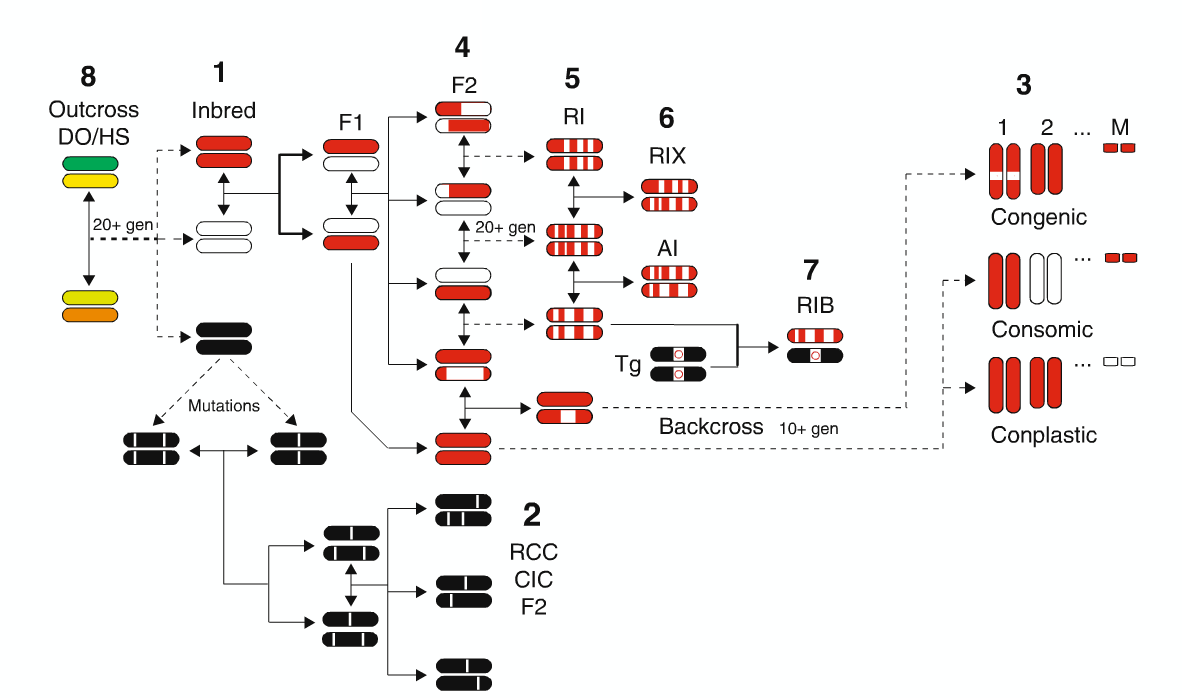
\includegraphics[width=\linewidth]{1.Introduction_Figures/BXDs.png}
		\caption{Adapted from:\citep{Williams2017ResourcesGenetics} Production of RI stock and validation of QTL results in congenic lines}
	\end{figure}
	
	The BXD mouse stock is generated from the crossing of C57BL/6J(B) and DBA/2J(D) mice. With repeated inbreeding of the offspring of particular F2 parents for 20 generations, distinct inbred strains can be developed. During this random and selective mating, recombinations events accumulate resulting in a thoroughly dispersed genomes in the mice resultant of the two parental breeds. Each strain is a distinct combination of the parental genomes which allows the construction of a matrix of allelic origins for each stretch of the strain genomes. Since each of the resultant strains accumulates relatively little spontaneous mutations in coding regions, it is sufficient to genotype the parents and reconstructed for the progeny. It is however an advantage that all BXD strains have been genotypes with the data available in several databases online.  In a study, many individuals of each BXD strain are used in order to have stability measured phenotypes which can be used for further QTL analysis \citep{Williams2017ResourcesGenetics}. 
	
	\subsection{Mouse Diets: Components of Chow and High Fat Diet}
	
    Diet is the major environmental factor controlled for between mouse cohorts in this study. The regular chow (CD) and high-fat(HF) diets exert significant separate and independent effects on the measured metabolites, proteins and transcripts and have to be controlled for in order to accurately map QTLs and evaluate $GxE$ interactions \citep{Warden2008}. Unfortunately, there is a variation in the composition of the feed between batches from the supplier and must be taken to account when compared metabolite data from different mouse studies.
	
    The chow diet used in this study is Harlan 2018, and the high-fat diet is Harlan 06414. As analyzed in Warden and Fisler, the dietary composition of the chow diet is as follows:  It is composed of agricultural products that represent a normal diet for mice and serves as a proxy for a healthy diet control in the mouse model population. It includes types of corn, wheat, oats and other grains and high fiber content from a range of vegetable sources containing complex carbohydrates\citep{Warden2008}. Additional protein and fats are added to the pellets from sources such as fish and vegetable oil \citep{Warden2008}. In contrast, the defined high-fat diet serves as a proxy for an unhealthy western diet in the model mouse population. As analyzed in Warden and Fisler, the high-fat diet consists of amino acid supplemented casein as it major protein source, cornstarch, maltodextrin or sucrose as the major carbohydrate components and fats from lard or soybean oil\citep{Warden2008}. Due to the lack of complex carbohydrates in the formulation, cellulose is added as a fiber source. Both diets are fortified with vitamins and minerals to ensure is mice in either cohort have the baseline requirements for proper functioning metabolism \citep{Warden2008}. 

	
	\subsection{Mouse Sex: Male and Female Mouse considerations}
	
    In a previous large BXD mouse experiment undertaken in the Aebersold, Auwerx and Zamboni lab, physiological differences between the two sexes of mice were investigated \citep{Andreux2012SystemsTraits}. Many variant traits are found but in subsequent studies, only male mice were used order maintain statistical power. In similar research conducted in other groups, the expansive literature of mice physiology is also biased. Male mice as often used in metabolic studies as they do not go through estrous cycles that can change their metabolic profiles\citep{Zucker2010MalesStudies} and female mice, however, analogous to female human have a longer lifespan on average as more often used in studies pertinent to identifying anti-aging mechanisms \citep{Yuan2011Miceaging}. In order to maximize the number of novel aging-related features detected in this study, a majority female mice population was used with a small male contingent for ensuring the factors found are not largely sex driven.
	
    Among the differences between the sexes in mice, one of the most pronounced contrasts to humans is the rapid estrous cycle mice experience. The reproductive cycle in humans, known as the menstrual cycle, lasts approximately one month. Analogous cycling in hormones and uterine physiology occurs every 4 to 5 days in mice and is known as the estrous cycle \citep{Caligioni2009}. Although these short cycles make mice ideal candidates for studying changes during reproductive cycles, they also present a complicating factor in assessing sterols and cyclic metabolites in metabolomic screens \citep{Zucker2010MalesStudies}. Estrous cycle data (ie. ovulation or cycle phase) is not included in the phenotypic observation of the mice in this study and as a result, may not be reliably excluded.
	
    An additional factor for using only female mice in this study are the large housing costs of keeping male mice in individual cages due to violent dominance behaviors. Male mice are extremely territorial and will even fight identical twins to the death if housed in the same cage. To keep males separates, however, has dubious animal welfare implications as lack of social interactions shortens the lifespans and increases stress levels of these social animals \citep{PeterKelmenson}. Barbering is another form of dominance behavior that mice show when housed together. The severity of barbering can change between individuals, but commonly includes the dominant animals physically aggressing others in the cage, particularly by plucking whiskers or tearing off hair and leaving large visible bald spots punctuated over the bodies of less dominant animals \citep{PeterKelmenson}. Although the behavior is observed in both males and female mice, it particularly common in female mice closely derived from C57BL/6 (B6) and A2G related strains \citep{Kalueff2006HairResearch} Both of these behaviors are a challenge of the technicians at mouse facilities, however barbering is preferential to male mice killing each other.
		
	\section{Why Multiple Omics}
	
    Large-scale inititatives to develop personlized medicine as standard therapy has driven a massive expansion in the number of human genomes that have been sequenced \citep{Telenti2016Deepgenomes, Fakhro2016}. With tens of thousands of human genomes with deep coverage \citep{Telenti2016Deepgenomes} and significant additional SNP variants mapping databases becoming available to public researchers, GWAS have become an important tool for evaluating the association between common genetic variants and risk of disease. Through signification efforts of the scientific community, thousands of disease associated SNPs have also been found\citep{Johnson2009AnResults.}. The results of many GWAS, however, are seldom followed up with investigations that probe biological mechanisms underlying the found associations and can explain a limited amount of heritability. Additionally, most SNP variants are associated with small increased risk probabilities of disease and thus have weak predictive value by themselves without additonal insight about the underlying biological mechanims. 
	
	\begin{figure}
		\makebox[\textwidth][c]{
		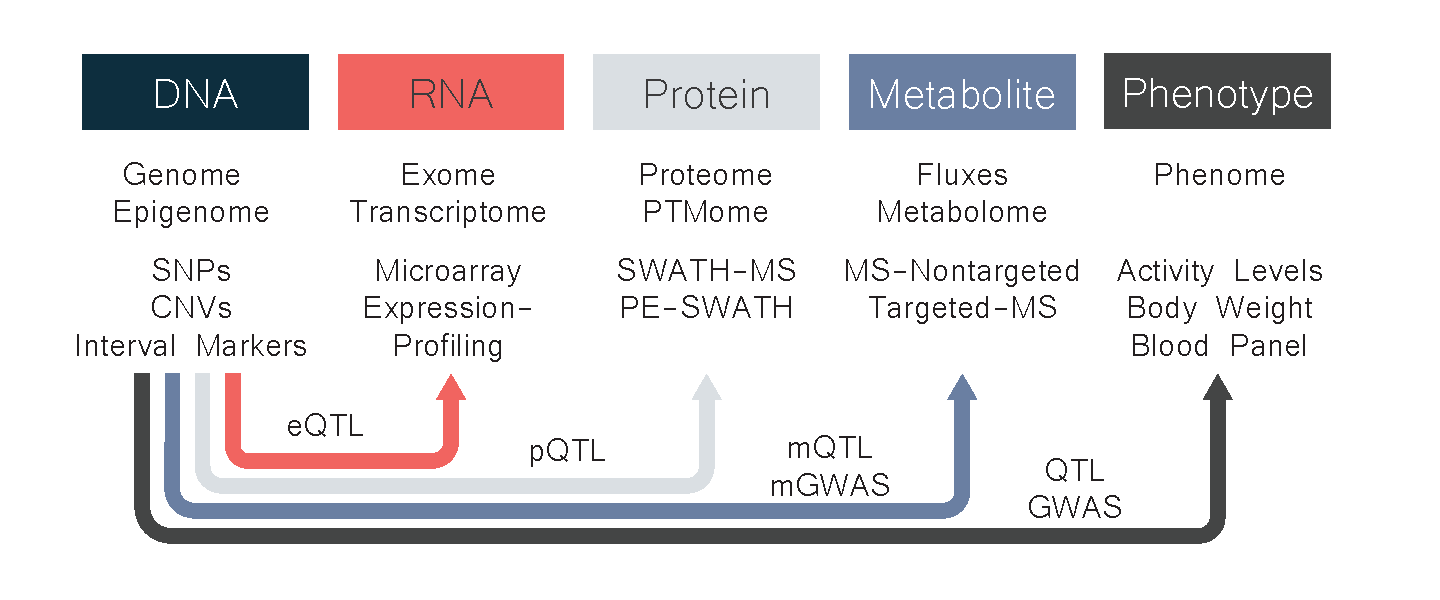
\includegraphics[width=1.2\textwidth]{1.Introduction_Figures/Multiomics.pdf}}
		\caption{Adapted from \citep{Dumas2012} Biological information that can be determined from performing high-throughput Omics analysis on many biomolecule read outs}
		\label{fig:Multi_Omics Methods}
	\end{figure}
	
    With maturation in other high-throughput omics technologies (Figure \ref{fig:Multi_Omics Methods}), orthogonal approaches can be used for mechanistic investigation of disease associations. Integration across different genomics, proteomics, transcriptomics, and metabolomics can comprehensively determine the relationships between genes, protein expression, metabolite concentrations, and their phenotypic repercussions as alluded to in figure \ref{Multi-Layer Trait Determination}. As observed in the previous BXD mouse study done by \citet{Williams2016SystemsFunction}, the levels of transcripts, their cognate proteins, and associated metabolites are only modestly correlation with each other. All three can also be further modified by enzymatic processes making good experimental design and optimization necessary to increase the resolving power of these investigations \citep{Johnson2016Metabolomics:Mechanisms}. 
	
	In order for us not to be overwhelmed by the large amount of data being collected, analysis will take place in a sequential layer by layer manner. First, the metabolite data is mined for QTLs and significantly enriched metabolites in the diet and age cohorts. From these metabolites we can determine which pathways maybe be affected by age, diet or a combination of two. Key enzymes that interact with the metabolites are preliminary hypotheses tested for differential expression at the proteomics level. If metabolite concentrations do not faithful correlate with proteins, mRNA data can be used. For example, if a accumulation of a metabolite is seen in a certain cohort of mice but there are no changes in the upstream enzyme concentration, RNA and genome data can lend an insight into whether there is a mutation in a coding frame withing the interaction enzymes and if there are activation effects of the high metabolites concentrations back on the RNA causing affecting the expression of the transcript. Ideally, structural learning techniques such as lingam\citep{ShimizuLiNGAM:Structures} can be used to validate the causal structures between all of the layers once a few causal network hypotheses have been generated.
	
	\chapter{Metabolomics}
	
	\section{Introduction to Non-Targeted Metabolomics}
	
	The metabolism is the sum of all the biochemical reactions that occur in an organism. Metabolites are shuttled through multiple enzymatically catalyzed reactions in the fundamental processes of energy production, growth and integrate multiple levels of information about the environment and cellular state in its kinetics and regulation mechanisms. The flux and relative concentration of these metabolites can be studied using multiple targeted and non-targeted techniques\citep{Aksenov2017GlobalSpectrometry}. 
	
    Unlike most common clinical assays, which are still photometric, the most common analytical techniques used to identify the global consortium of metabolites present in a cells or tissues are NMR and mass spectrometry based \citep{StanfordBloodTests}. The goal of non-targeted metabolomics is to detect and quantify as many metabolites from a single extracted sample as possible without prior knowledge of the specific composition of the metabolome. Although, chromatographic separation steps can be used to differentiate between a specific set of compounds inseparable with a single mass spectrometry step, due to analytical limitations, a single analysis cannot be used to cover the total metabolome which may consist of thousands of molecules with highly variable physiochemical properties. As a result, a decision must be made to determine the most pertinent class of compounds to best address the biological question and a sample is processed according to a protocol optimized for that small portion of the metabolome. Normally protocols for quantifying small polar molecules capture most of the central metabolism and provide an overview of metabolism but cannot resolve ratios between many enantiomeric and diastereomeric compounds like sugar or lipids \citep{FGCZ2017MetabolomicsZurich}. As a result, metabolomics, unlike genomics or proteomics is subdivided into many disciplines such as small polar molecule metabolomics, lipidomics, and glycomics focusing in different chemical classes of compounds which can be effectivly analysed useding similar processing and analytic techniques \citep{FGCZ2017MetabolomicsZurich}.
	
    Although the types of metabolites recovered in different experiments may be structurally distinct, the result is always complex data that require signal analysis and cheminformatics tools to process the raw signal from the mass spectrometer into peaks that can be assigned a normalized intensity and a chemical annotation. Bioinformatics and statisticaly analysis tools are then required to determine the correlation between metabolites in the given modules of the metabolites and to examine the connectivity of these metabolic pathways in the context of a phenotype or a process that may be driving a disease\citep{Aksenov2017GlobalSpectrometry}.
	
	In contrast to untargeted mass spectrometry, targeted metabolomics operate on prior knowledge and hypotheses and quantify molecules of specific properties and mass ranges. The chromatography step before the mass spectrometry is optimized for extracting and separating the target metabolites and pathways such as the hexose sugars in glycolosis or lipids with equals masses but differences in the locations of their unsaturations \citep{Cani2009}. Targeted analysis can therefore be used as a follow up to untargeted metabolomics in order to validate hypotheses or quantify specific functional isobars(molecules with distinct  properties but identical mass to charge ratios) such as enantiomers or diasteriomers.
	
	The way to perform flux analysis differs on the class of molecule, but generally, a isotopically labelled carbon, nitrogen or oxygen within a metabolite can shed light on which pathways that metabolites is shuttled into\citep{Zamboni200913C-basedAnalysis}. Seeing an isotopic wight shift within pyruvate and different amino acids can quantify the utilization of glucose in anabolic and catabolic reactions. Ideally, one would use tracer compounds to directly quantify the fluxes of all metabolites in a multiplexed fashion, however this is unfeasible because it is technical difficulty and very expensive \citep{Zamboni200913C-basedAnalysis}. 
	
	
	\subsection{Metabolomics Methods}
	
	Metabolomics combines analytical chemistry and mass spectrometry platform technology, with sophisticated data analysis for deconvoluting dense MS1 broadband spectra. It involves the application of chemo and bioinformatics tools to profile the diverse metabolic complement of BXD mouse livers and put the results in biologically relevant context \citep{Coen2010}. Even with few standard tools and piplelines, metabolomics still offers a platform for the comparative analysis of metabolites that reflect the dynamic processes underlying cellular homeostasis\citep{Aksenov2017GlobalSpectrometry}.
	
	\begin{figure*}[hbt!]
		\makebox[\textwidth][c]{
		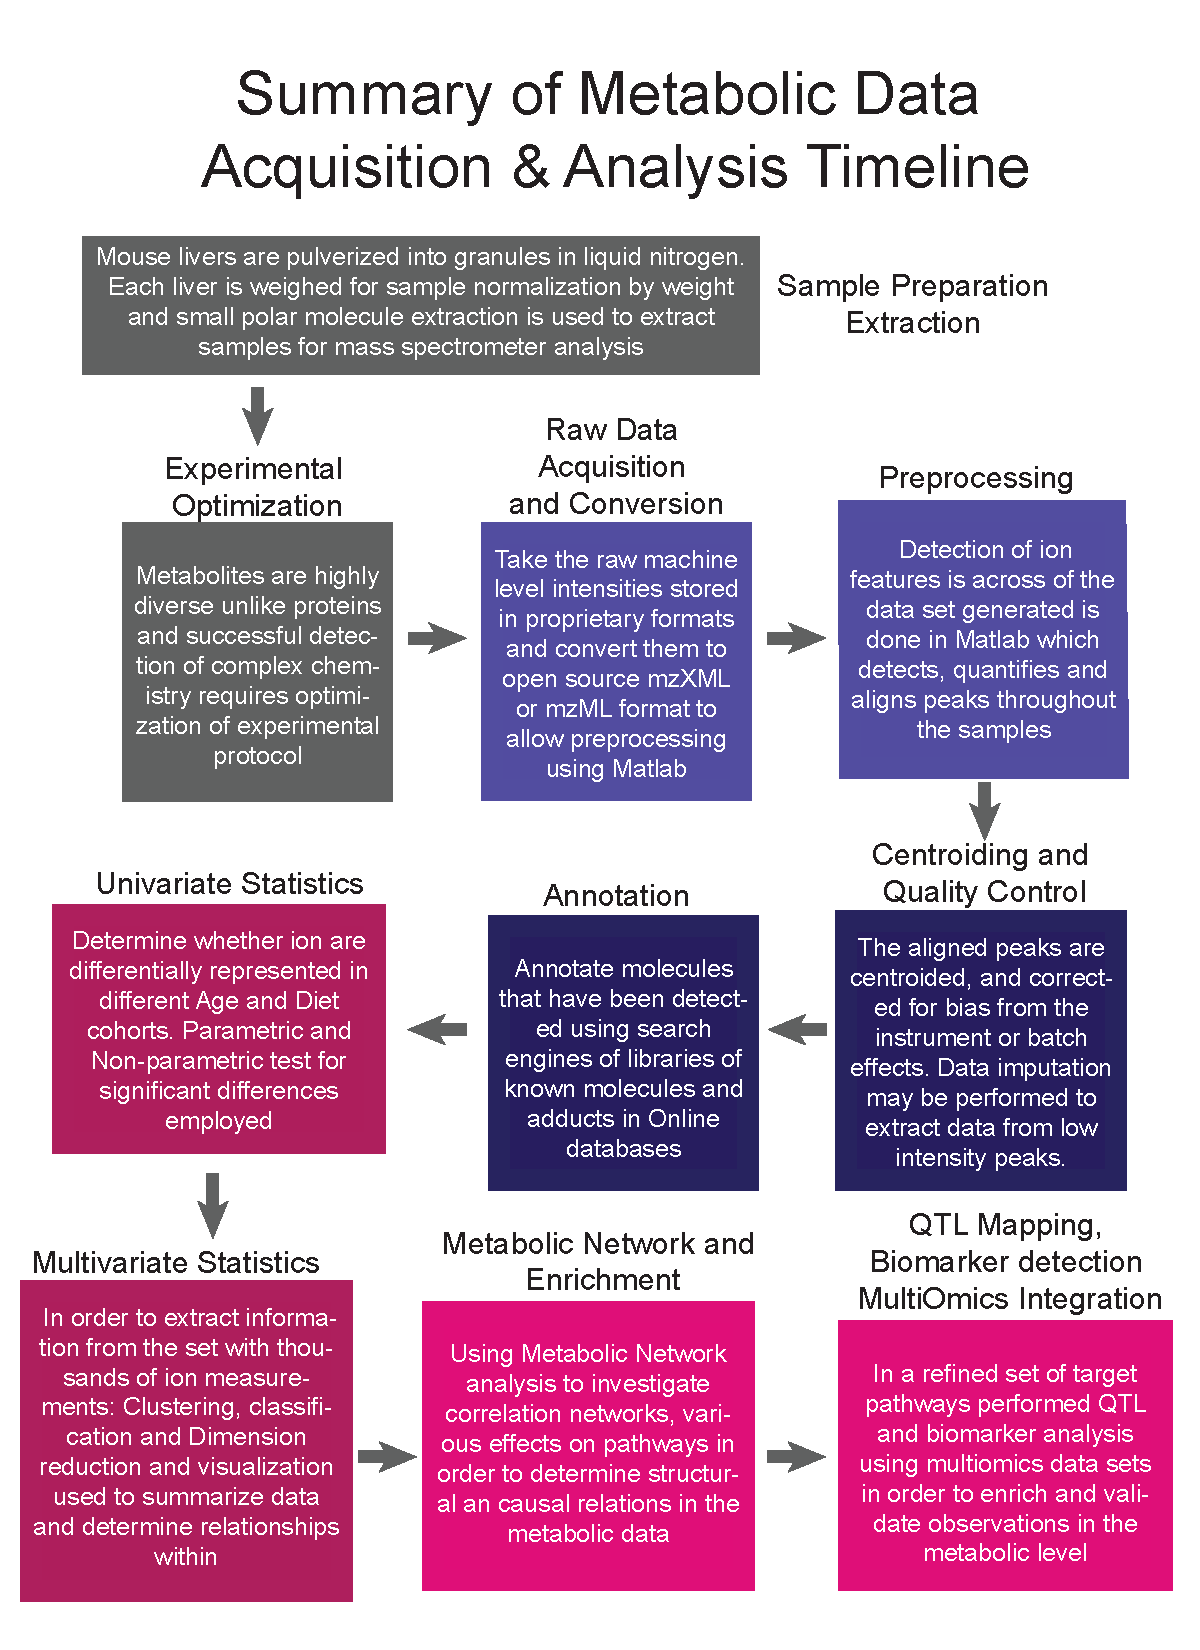
\includegraphics[width=1.2\linewidth]{3.Metabolomics/pipeline.pdf}}
		\label{OverviewMetabolicsPipe}
	\end{figure*}
	
	MS-based metabolomics offers high selectivity and sensitivity for the identification and quantification of metabolites. Substantial progress in the speed and resolution of instruments and sampling processing techniques used in metabolomics has significantly broadened its analytical capabilities \citep{Aksenov2017GlobalSpectrometry}. Additionally, new orthogonal separation techniques like differential ion mobility spectrometry add seconds to the overall analysis while allowing the separation of a wide range of isobars \citep{Domalain2014EnantiomericSpectrometry}.In addition to the technical developments of metabolomics mass spectrometry, a range of chemoinformatic tools and databases that reduce the complexity of data processing, handing\citep{Xia2016UsingAnalysis}, annotating signals for complex metabolites adducts and provide context to the metabolites within different biological pathways\citep{Wishart2013HMDB2013,Xia2010MSEA}. In the metabolomics studies described in this thesis, a high resolution TOF instrument is used, generating more than 17000 peaks in the mass analysis. Of these peaks around a 1500 can be annotated. A road-map of the full metabolite analysis pipeline is given on the next page.
	


	\section{Metabolite Extraction Protocol \& Optimization}
	
	The experimental protocol for small polar molecule extraction and sample preparations from mouse liver is very simple in comparison to other metabolite classes and mass spectrometer analytes\citep{Mushtaq2014ExtractionMetabolome,Haynes2009Sphingolipidomics:Sphingolipids,Hu2009AnalyticalDiscovery}. The liver tissue is homogeneous, comprising mostly of hepatocytes which can be effectively ground to a powder in \ch{N2_L}, which enables rapid extractions. The pulverized liver tissue is lysed with a combination of \ch{H2O}, \ch{MeOH} and \ch{ACN} after which homogenization and different extraction times can be used to extract the metabolites from the slurry. 
	
    To ensure the reproducibility of experiments chemical or enzymatic reactions that may occur during the tissue extraction must be minimized because these can drastically alter the original metabolite profile of the organism\citep{Mushtaq2014ExtractionMetabolome}. This rapid inactivation of all biochemical and enzymatic activity in organisms is known as quenching and is performed by a the \ch{MeOH} and \ch{ACN} in the extraction solution denaturing the proteins in the sample. In low-temperature extractions, long extraction times can be used without large changes from thermal degradation. Short extraction times in high-temperature extractions are used to prevent spontaneous chemical reactions. 
	
    Once the metabolites are extracted, the samples are evaporated in a low-pressure centrifuge and can be stored. Small molecules show much higher reaction kinetics than peptides and must be dried to a pellet and stored at -80$^{\circ}$ until they need to be resuspended and analyzed. On the day of analysis, the samples are resuspended at concentrations of 5\si{\milli\gram\per\milli\litre}into 96 well plates and loaded into the auto-sampler for randomized sampling into the mass spectrometer.
	
	\subsection{Optimization Objectives}
	
	Processing 600 samples in a single run is an extremely time consuming process and required at least 20\si{\milli\gram} of the precious mouse livers samples. Small scale pilot studies were used to determine whether the metabolite extraction protocol used in the previous paper\citep{Williams2016SystemsFunction} were reliable and reproducible 3 years after the experiments were done. Moreover, we had a limited amount of mouse liver, certain amounts of which had to be allocated for proteomics and transcriptomics and reproduction experiments should reviewers ask, thus it was imperative to conserve material. 
	
    Additionally, we wanted to tune the protocol to maximize the intensities and reproducibility of the metabolite data. Differential detection of key discriminant metabolites (such as N6-methyl lysine found in significantly higher quantities in chow diet mouse metabolites and has a strong known QTLs) which were observed in previous publications of the BXD mouse data was used to benchmark our current protocol \citep{Williams2016SystemsFunction,Wu2014MultilayeredPopulation}.  A timeline of all the metabolite studies is given below.
	
	\begin{enumerate}
		\item Pilot Study 1 - The first pilot study is used to determine the difference between hot and cold metabolite protocols and extraction time dependence on the metabolites intensities.
		\item Pilot Study 2 - The second pilot study is used further refine the time schedule of the extractions and generate a standard curve with response factors for each metabolites. 
		\item Full Run 1 - The first full run with all 600 mice samples is done using the cold extraction protocol optimized in with first two pilot studies 
		\item Full Run 2 - follow up full run was performed due low number of features detected and sporadic jumps in the total ion counts in the first full run , yielding much higher coverage and lower CVs 
	\end{enumerate}
	
	\section{Pilot Study 1}
	
	Four extraction conditions were tested, a hot extraction, two cold extraction and one homogenization free extraction, to determine which steps contributed to optimal extraction efficiency and robust metabolic coverage. The boxes outlined in red in figure \ref{fig:Hot Extraction Protocol} are the steps under scrutiny in this pilot study.
		
	\subsection*{Hot Extraction:}
	
	\begin{figure}[b!ht]
		\centering
		\fbox{ 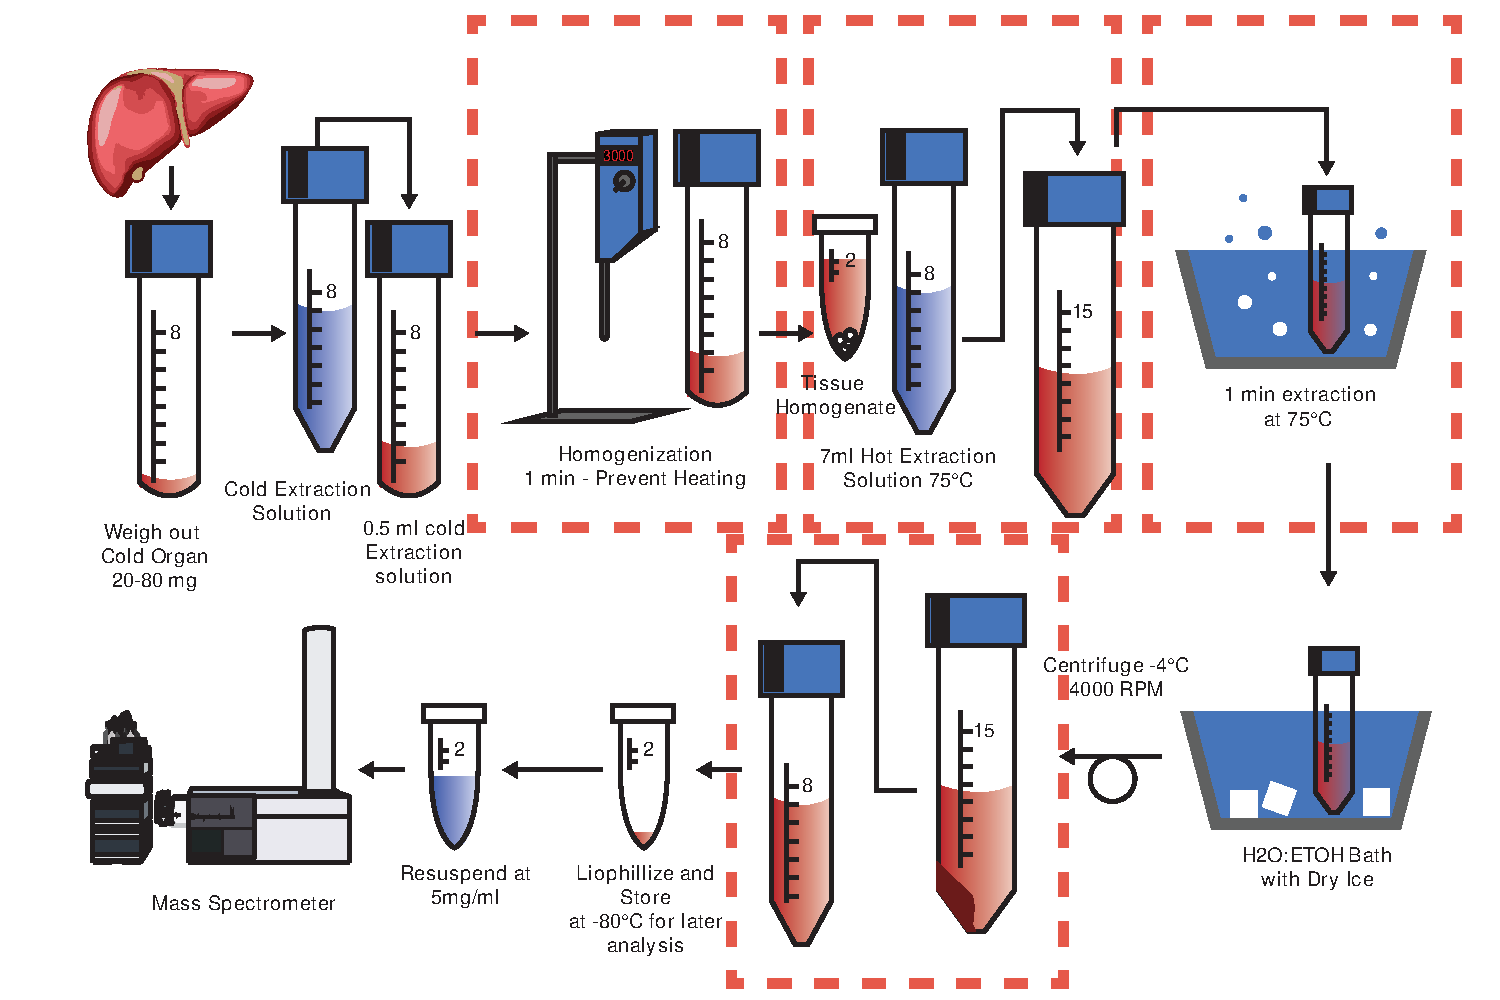
\includegraphics[width=1\linewidth]{3.Metabolomics/Procedure.pdf}}
		\caption{Hot Polar Metabolite Extraction Protocol}
		\label{fig:Hot Extraction Protocol}
	\end{figure}
	
	
	In a hot extraction protocol (Figure \ref{fig:Hot Extraction Protocol}), liver samples kept at -20$^{\circ}$ on dry ice are weighed into cell culture or falcon tubes. The tubes must be no longer than 10cm long to allow for the homogenization head to reach the bottom of the tube. After weighing, 0.5mL of extraction solution is added to the samples. The extraction solution is sufficiently membrane disrupting and dissolves cellular membranes freeing the metabolites. 
	
	A homogenization step using a laboratory-grade blender is included in the protocol to further lyse cells and break up particulates of protein and other non-polar cellular debris that may crash out of the solution. During this process, viscous heating from the homogenizer brings the sample temperature up quickly. Thus the sample must be rapidly transferred into falcon tube with 3.5mL of extraction solution at 75$^{\circ}$ and timed for a minute. Although the original protocol calls for an 8ml final volume of extraction solution, 4ml of extraction solution was used because it would take less time to evaporate. To minimize degradation and restarting enzyme-free metabolism, timing is kept meticulously ensuring the sample does not have elongated exposure to high temperatures. 
	
	After a minute, the samples are removed from the hot bath and placed into a -20$^{\circ}$C bath to quickly cool the tubes. At this temperature, it is assumed most metabolic reactions have stopped and can be kept at his temperature while the rest of the samples are being processed. The samples are then centrifuged to remove high molecular weight materials and the supernatant evaporated.The metabolite powder is stable at -80$^\circ$C and can be resuspended later on the day of analysis.
	
	\subsection*{Cold Extraction:}
		
	The cold extraction (Figure \ref{fig:Cold Extraction Protocol})is similar to the warm extraction. 4ml of a [40:40:20] solution of \ch{MeOH}, \ch{ACN} and \ch{H2O} is added directly to the sample to solubilize cells and poison enzymes. The samples are then homogenized and immediately put into a cold bath afterward to bring the temperature down to -20$^\circ$. The tissue samples are then left to sit in the solution or in the fridge at -20$^{\circ}$C to allow further extraction. Two cold extraction times were used, 1 hour and 24 hours at -20$^{\circ}$CC to determine the extraction kinetics and optimal extraction times. 
		
	\begin{figure}[hbt!]
		\centering
		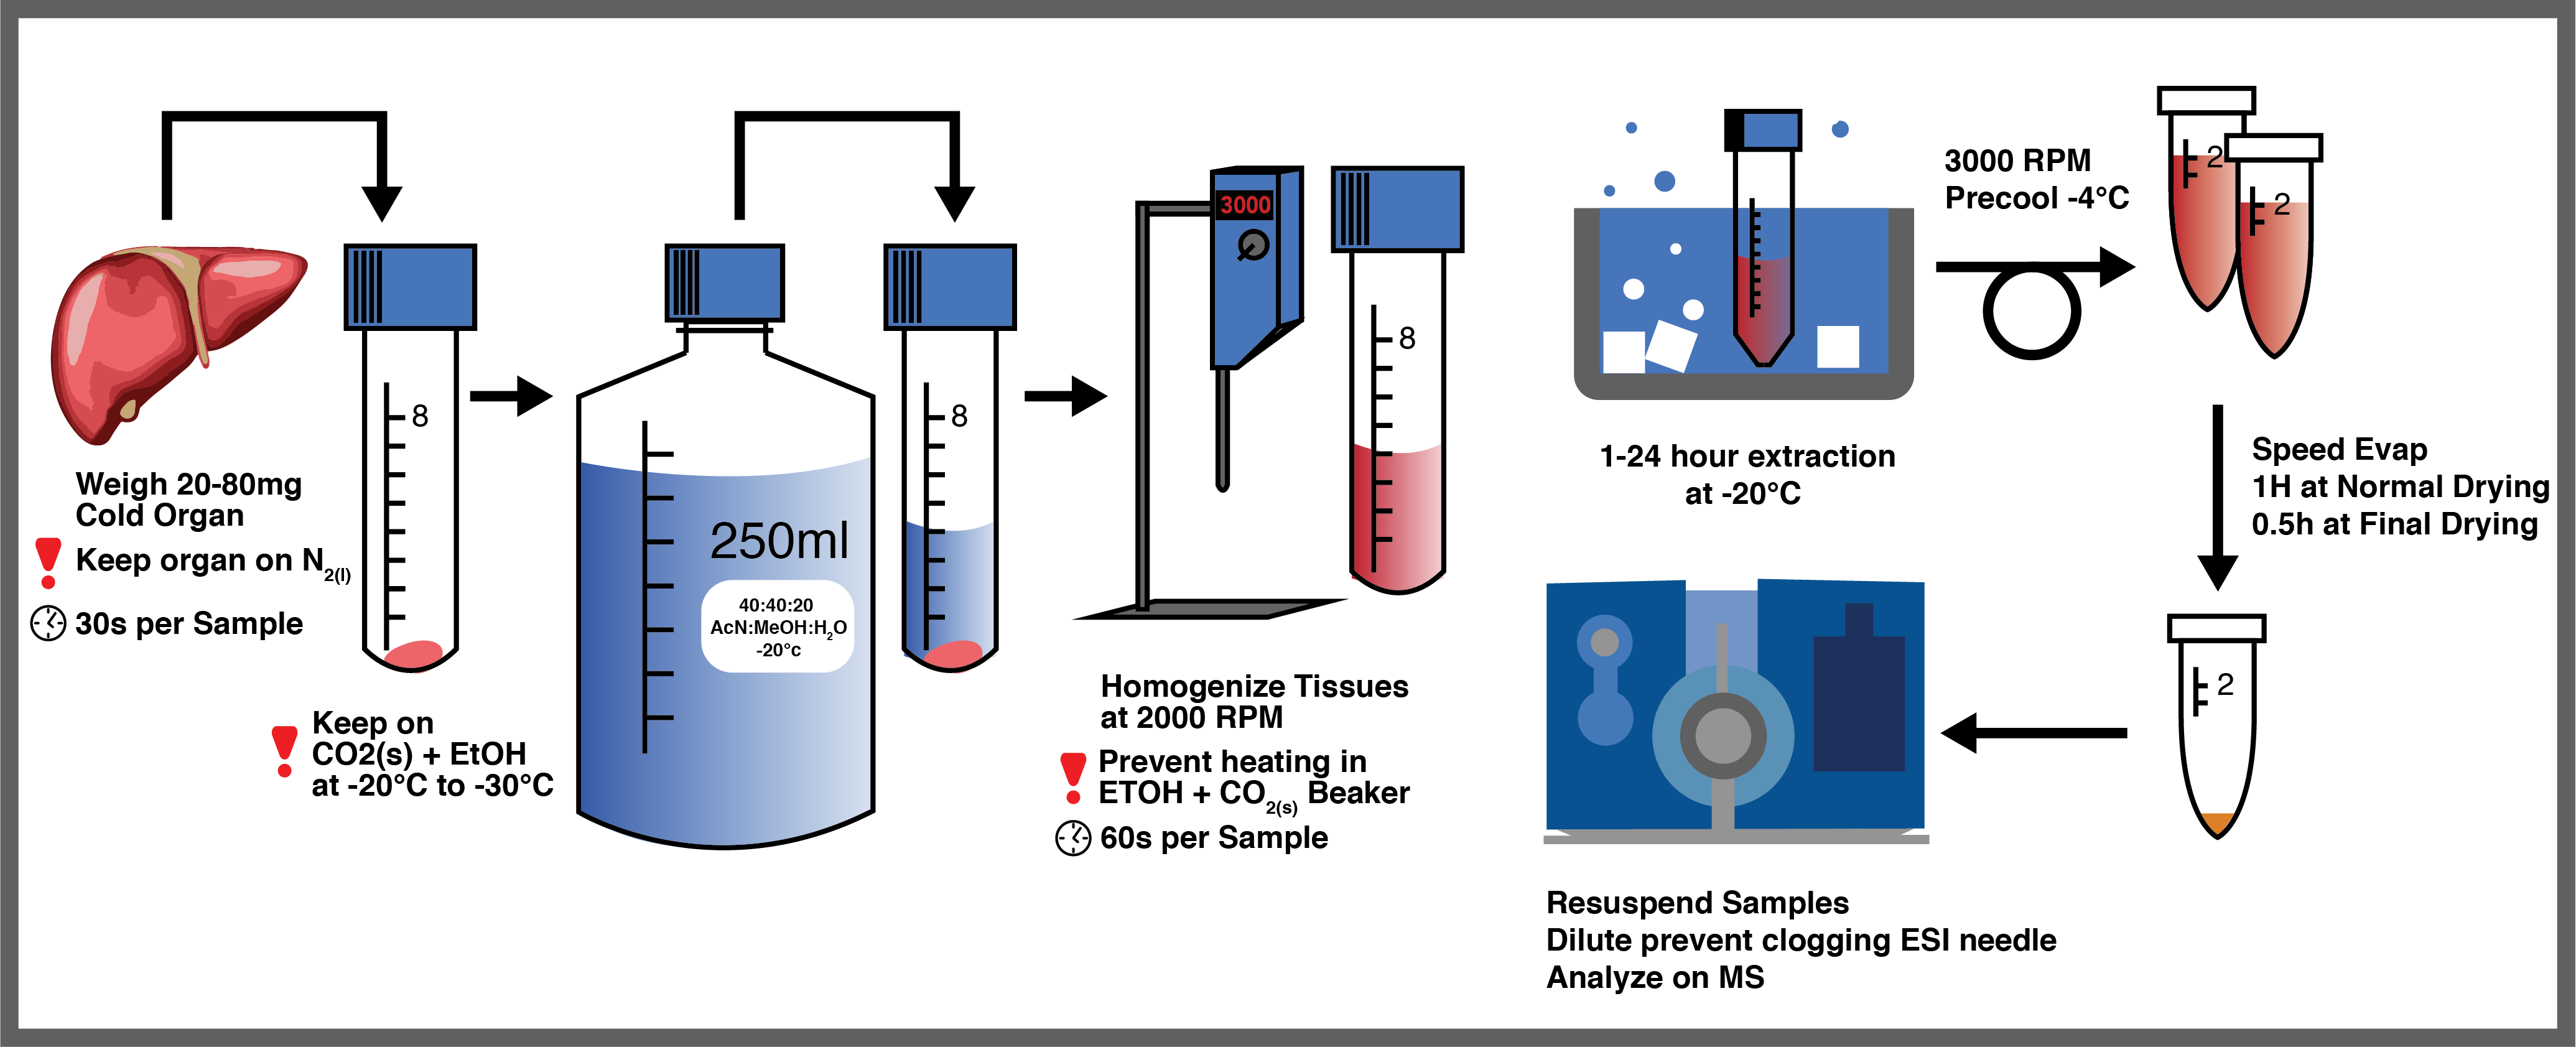
\includegraphics[width=\linewidth]{2.Optimizaiton_Figures/Metab-Cold-Proto-MH-20170120}
		\caption{Cold Polar Metabolite Extraction Protocol}
		\label{fig:Cold Extraction Protocol}
	\end{figure}
		
	\subsubsection*{Homogenization-Free Cold Extraction:}
	
    In most analytical extraction homogenization is usually recommended to achieve an effective extraction\citep{Mushtaq2014ExtractionMetabolome}. As the complexity and resilience of the tissue increases, homogenization becomes a crucial step for breaks apart colloidal collections of cells, in the centers of which are not exposed to the extraction solvent. Moreover, metabolites are present in different compartments of cells, thus the disruption of those cells or their protective covering can maximize the extraction of metabolites. Liver tissue, however, contains a low diversity of cell type and is not difficult to break apart unlike muscle tissue. As a result, there may not no additional benefit to the metabolite extraction effectiveness in liver tissue with homogenization.

	There are several techniques that can be used separately or in combination to homogenize samples. The most conventional, grinding the liver tissue manually with a mortar and pestle is performed on all of the tissues samples. However, in the protocol described by \citeauthor{Williams2016SystemsFunction} an additional homogenization step with a laboratory mill ball or laboratory-grade blender is called for after the cell lysis/quenching and extraction solution is added to the tissue. The lab-grade blender in the Aebersold lab can effectively liquefy tissue samples, however, the temperature of the samples is raised and cross-contamination occurs reduced the resolution power of low abundance metabolites. Although ultrasonication can also be considered as an alternative to high-speed mixers or strongly agitated ball-mills, the low numbers of sonicators in our lab precludes the use ultrasonication on 600 samples.

	Already, leaning towards using the cold extraction due to its simplicity, we also performed a 24 hour cold extraction without the homogenization step to determine if it was necessary. The homogenizer step introduces impurities and cross-sample containments if the homogenization head is not properly cleaned and adds a minute to each protocol, complicating the timing of the protocol. Thus warranting us to determine if it can be circumvented.
	
	\section{Pilot Study 1 Results}
	
	\begin{figure}[!ht]
		\centering
		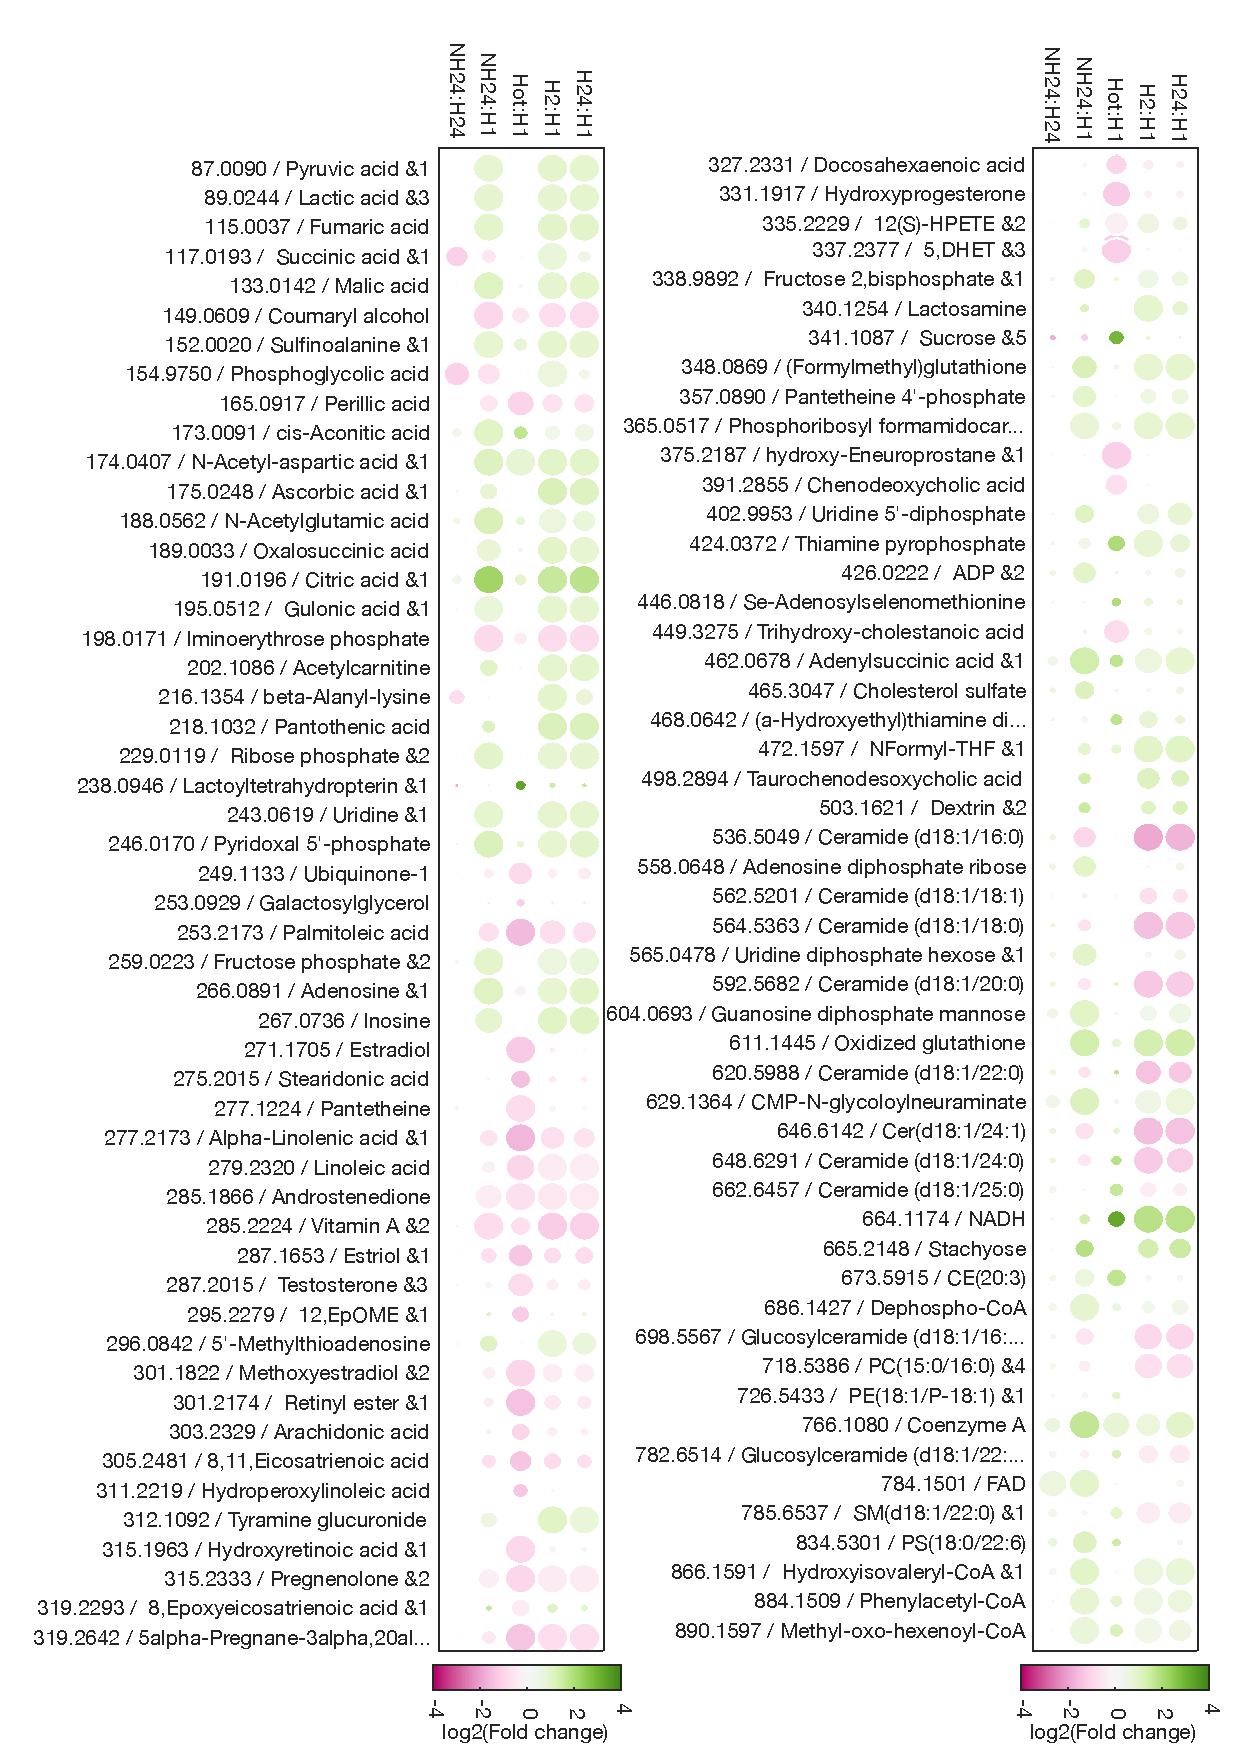
\includegraphics[keepaspectratio,height=.8\textheight]{2.Optimizaiton_Figures/bubbles1.pdf}
		\caption{Metabolites $Log_2$ fold changes between different extraction conditions. Hot - indicates the hot extraction used in the Science paper, H1 in the cold extraction with a 1 hour extraction  time, H24 also the cold extraction but with a 24 hour extraction time, NH24 is the cold extraction with 24-hour extraction without the homogenization with the lab-grade blender}
		\label{fig:Pilor Study 1 Bubble Chart Results}
	\end{figure}
	
	\subsection*{Hot and Cold Extraction Performance}
    The intensities from a sampling of metabolites across the 50-1000 Dalton m/z range is given in figure \ref{fig:Pilor Study 1 Bubble Chart Results}. In the third column, the Hot:H1 column compares the intensities seen in the standard hot extraction with the metabolites extracted using the cold extraction protocol with a 1 hour incubated at -20$^\circ$C. In the lower mass range, the effect is minuscule between the group with significant differences appearing in lipids and cholesterol species that are difficult to extract quantitatively without the use of glass cuvettes that have a polar activated internal surface \citep{Xia2010}. Almost all of the highlighted metabolites in the \hyperref[volcano plot: Hot_vs_Cold_H1]{volcano-plot (figure \ref{volcano plot: Hot_vs_Cold_H1})} are thus not of primary interest.

	\begin{figure}[htb!]
		\centering
		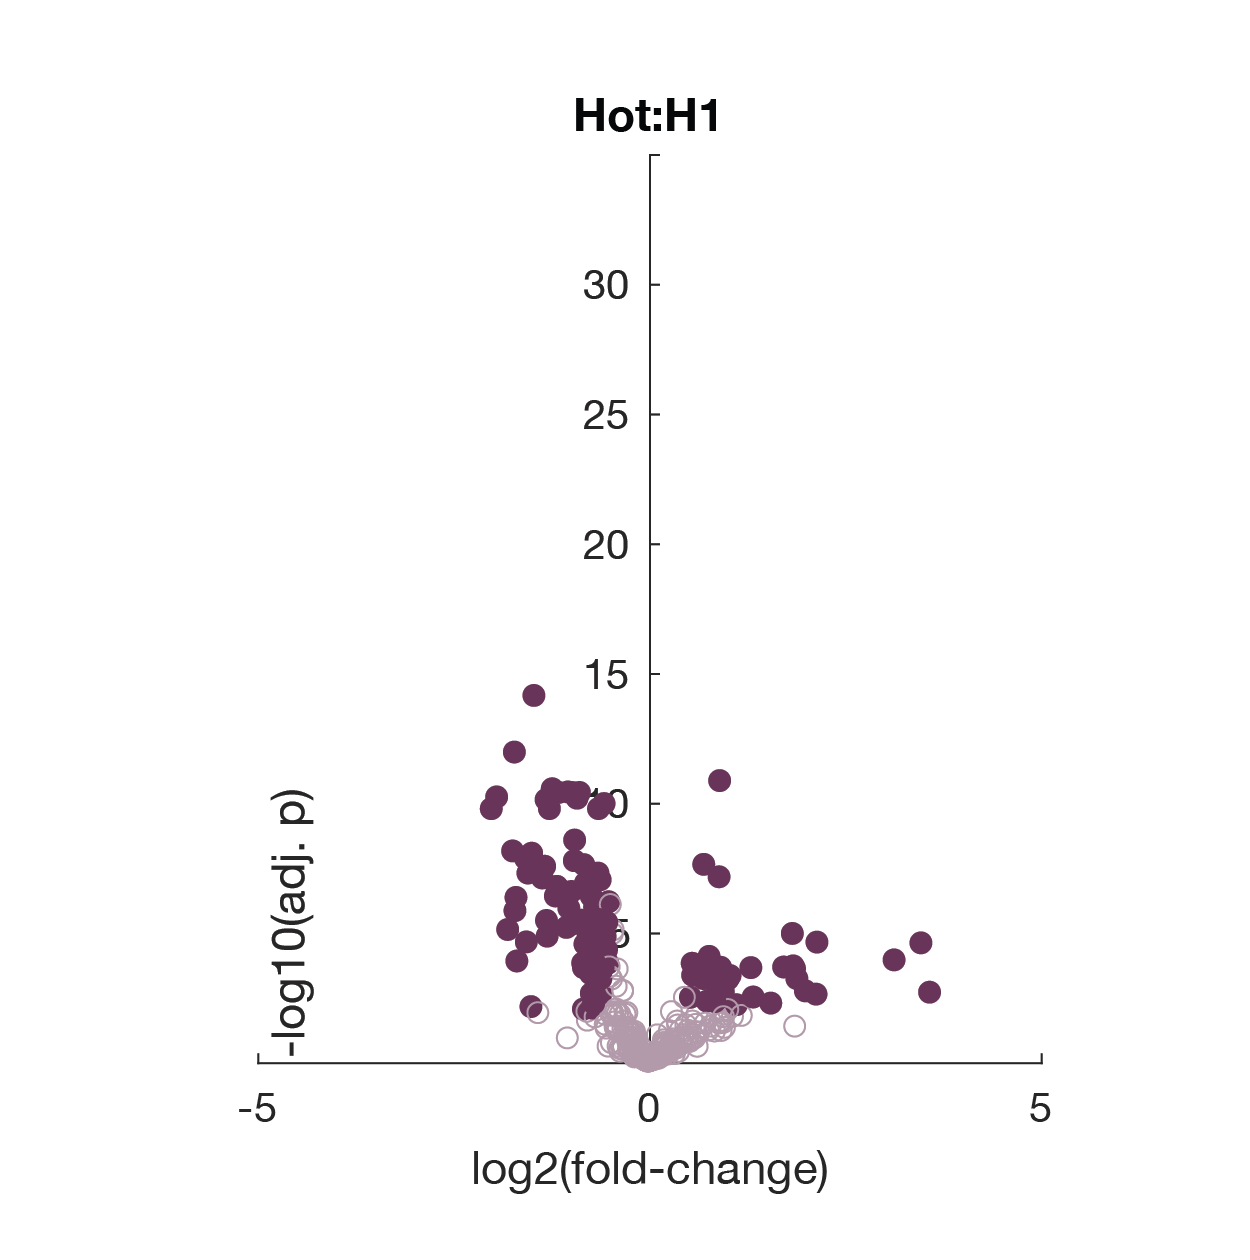
\includegraphics[=\linewidth]{2.Optimizaiton_Figures/Hot_H1_01}
		\caption{Volcano Plot of P-Values and Log2 Fold Changes seen between Hot Extraction protocol and Standard Cold Extraction Protocol}
		\label{volcano plot: Hot_vs_Cold_H1}
	\end{figure}
	
	\subsection*{Time Dependence of Cold Extraction}
	Results shown in figure \ref{volcano plot: 24h, 1h and 2h cold extraction comparisons} show that both 2 and 24 hour cold extractions extract a higher number of metabolites that the 1 hours protocol. There is a higher variation in the extraction metabolites seen in the 2 hours extracting. One can conjecture this arises from insufficient extraction times, however, the original protocol used in \citep{Williams2016SystemsFunction} used 10-minute extraction, so coming to this conclusion is questionable. 
	
	\subsection*{Extraction Time Performance}
	\begin{figure}[htb!]
		\centering
		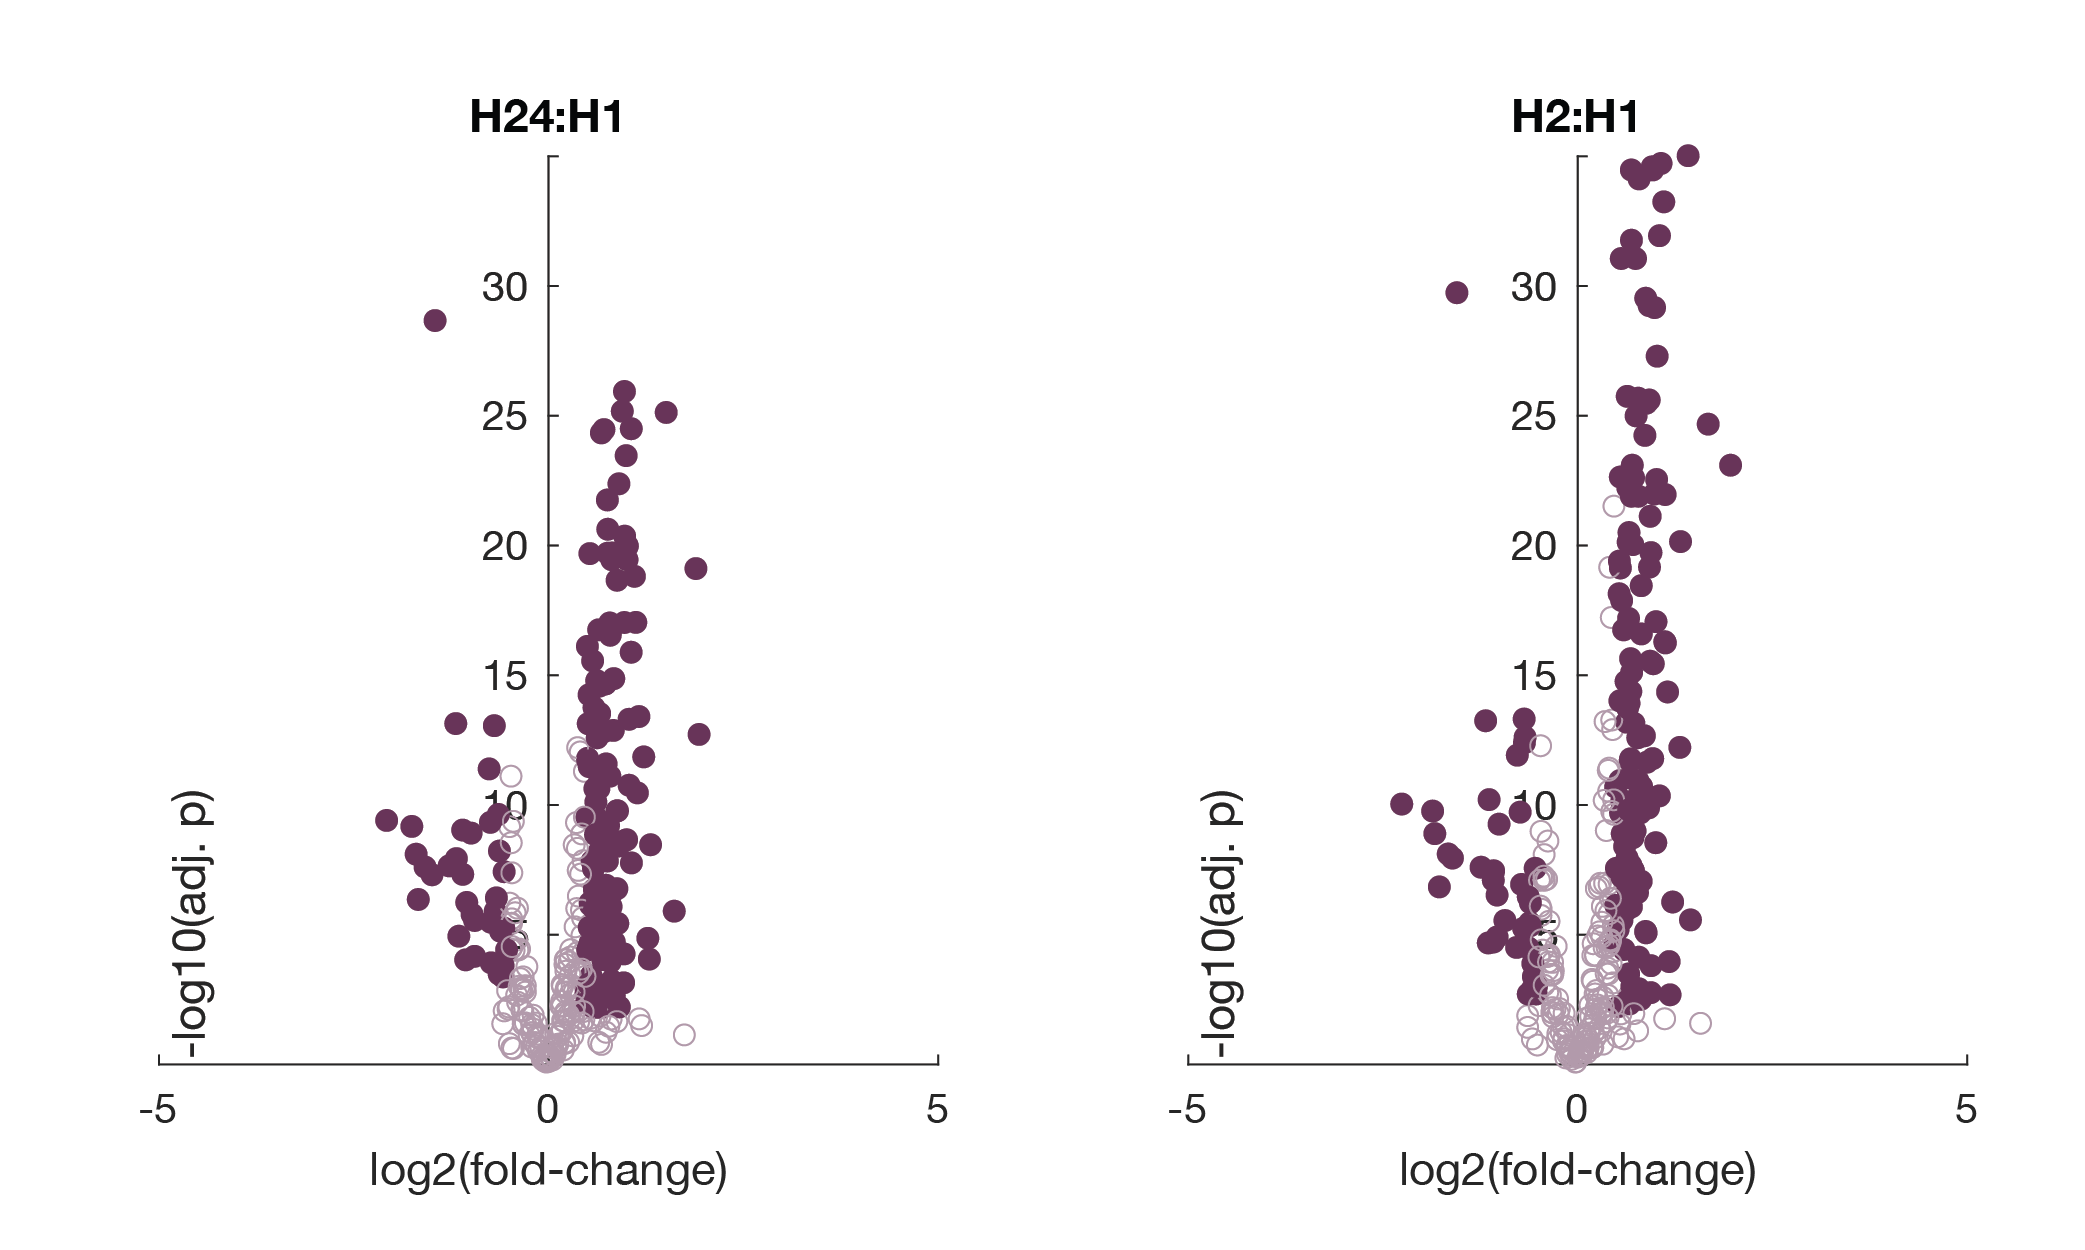
\includegraphics[width=\linewidth]{2.Optimizaiton_Figures/H1-H24-H2-01}
		\caption{Volcano Plot of P-Values and Log2 Fold Changes seen between Standard Cold Extraction Protocols with an additional 1hour and 24 hour extraction period as compared to the standard cold extraction protocol}
		\label{volcano plot: 24h, 1h and 2h cold extraction comparisons}
	\end{figure}
	
	\subsection*{Effect of Homogenization on Performance}
	
	To recall, the liver tissues are already pulverized in a mortar and pestle before all of the extractions. The effects of an additional lab-grade blender homogenization, as required in the \citeauthor{Williams2016SystemsFunction} protocol were tested in a 24 cold extraction done with and without the additional homogenization step. From the volcano plots (figure \ref{volcano plot: Effect of Homogenization of Metabolite Extraction}) , it can be seen that homogenization does not significantly increase the intensities of metabolite profiles. Surprisingly it actually reduces the metabolite intensities and increase the CV by 4\% (not shown) in the cold extraction, although the source of this variability is not clear.
	
	\begin{figure}[!htb]
		\centering
		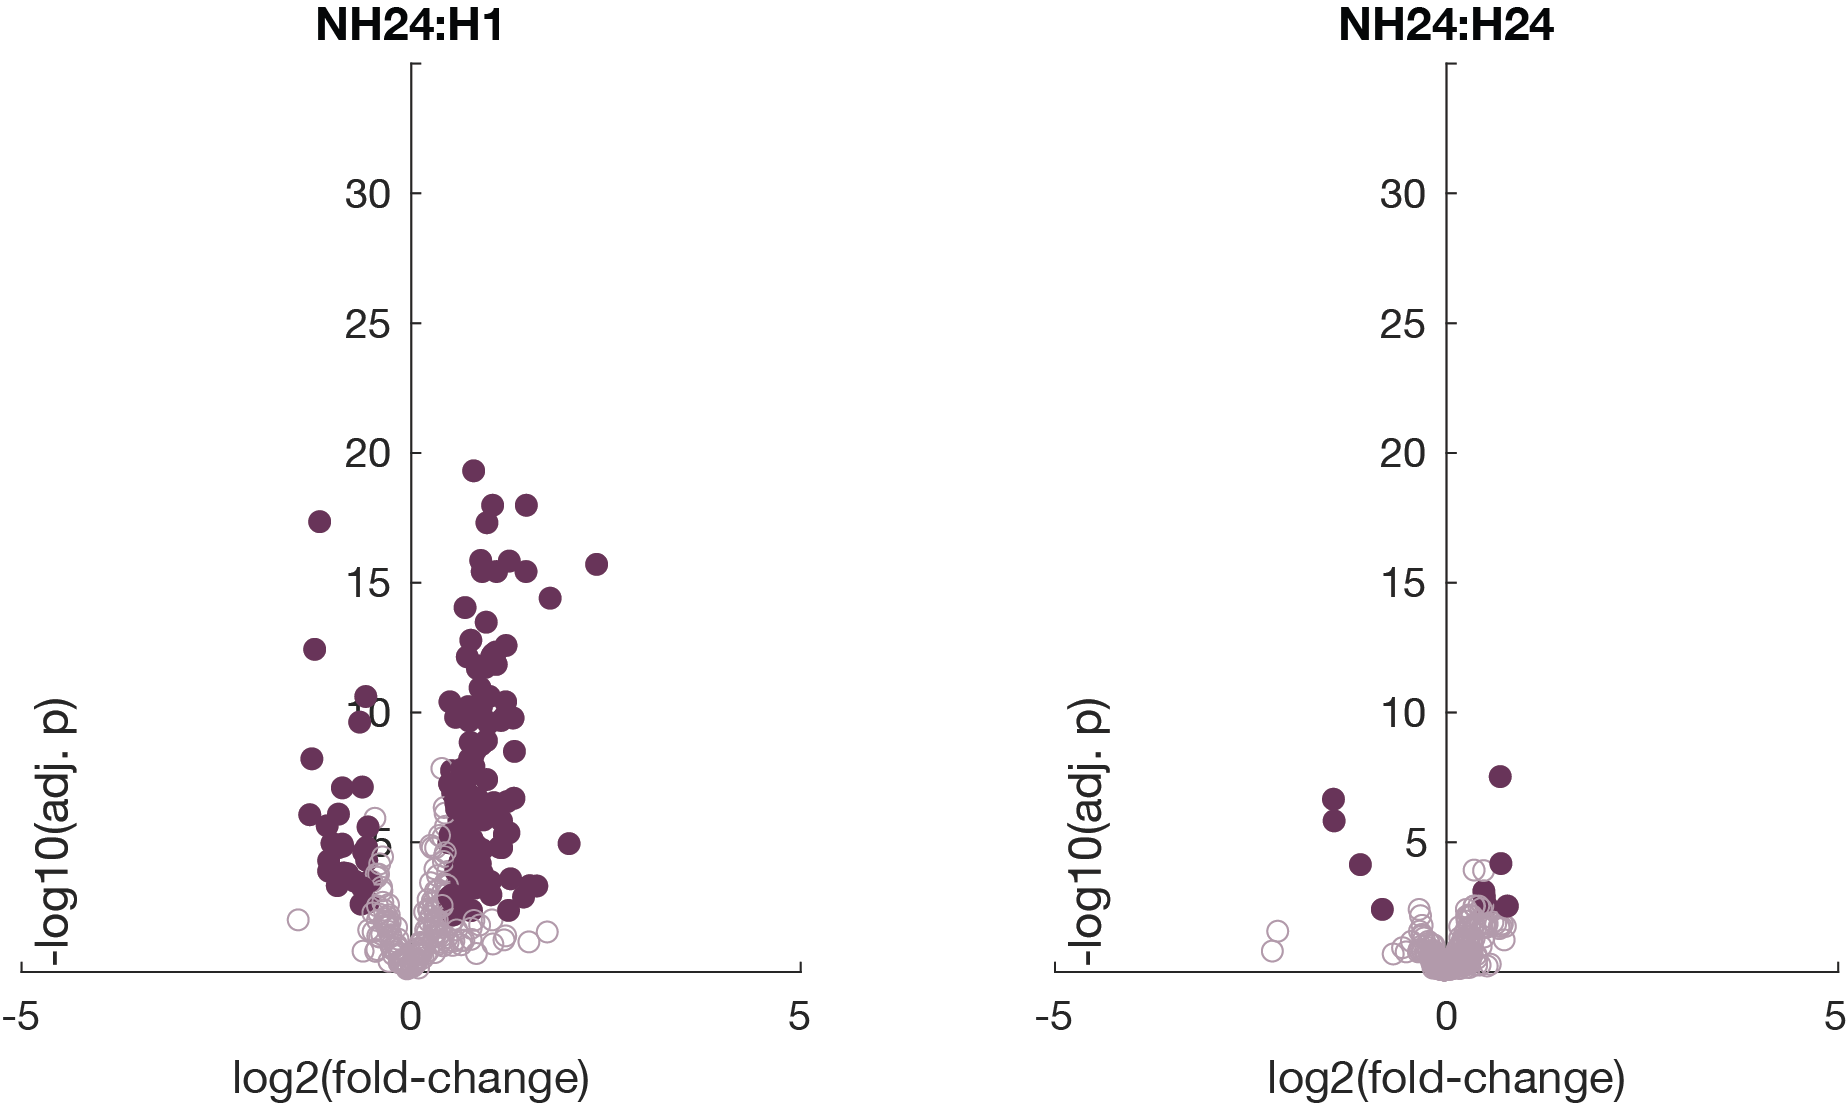
\includegraphics[width=\linewidth]{2.Optimizaiton_Figures/NH24}
		\caption{Volcano Plot of P-Values and Log2 Fold Changes seen between Standard Cold Extraction Protocols with an additional 1hour and 24 hour extraction perdion as compared to the standard cold extraction protocol}
		\label{volcano plot: Effect of Homogenization of Metabolite Extraction}
	\end{figure}
	
	\subsection*{Pilot Study 1 Conclusions}
	
	as a result of the first pilot study, the homogenization step is taken out of the protocol. We also found that the hot extraction and cold extraction yield similar results, thus the hot extraction was supplanted by the cold extraction is it reduces the need for cumbersome heaters to maintain the high extraction extraction solution and extraction bath. Although we know longer extraction times give higher metabolites intensities, the optimal extraction schedule is still unclear as many significant metabolites found in the Science paper \citep{Williams2016SystemsFunction} were missing from the first optimization
	
	\newpage
	\section{Pilot Study 2}
	
	The second pilot study was aimed at tuning a range of parameters for the cold extraction and maximizing metabolites quantified and their intensities.

	\subsection*{Pilot Study 2 Objectives}
	 
    Biological replicates, of mice in the same age cohort, diet and strain were also included to determine which metabolites were most reproducible between biologically identical" mice.  A freeze-thaw cycle experiment as performed in order to determine if there are any detrimental effects of freezing metabolites suspended in water. This was done to ensure the sample would be usable in case the samples would need to be frozen overnight and the extraction continued the next day due to unforeseen circumstances. lastly, separate blank samples containing ultrapure millipore water were included for every 10 samples on the 90 well plate for flushing the sample input lines in the mass spectrometer. It is thought this would decrease the baseline noise intensities in the mass spectrum profiles and reduce cross-contamination between samples.
	
	\subsection*{Extraction Time Optimization}
	
    In the previous Pilot study 1, the cold extraction was chosen of the hot extraction as it extracted a similar number of metabolites, with higher intensity and had fewer processing steps. However, only 1 hour and 24 hour extraction times were examined across all 24 samples in the pilot study. In order to determine the optimal extraction kinetics for the cold, a time series experiment was conducted. The samples were prepared using the cold extraction methods and allowed to incubate from times between 1 minute and 3 days.
	
	\begin{figure}[ht]
		\makebox[\textwidth][c]{
		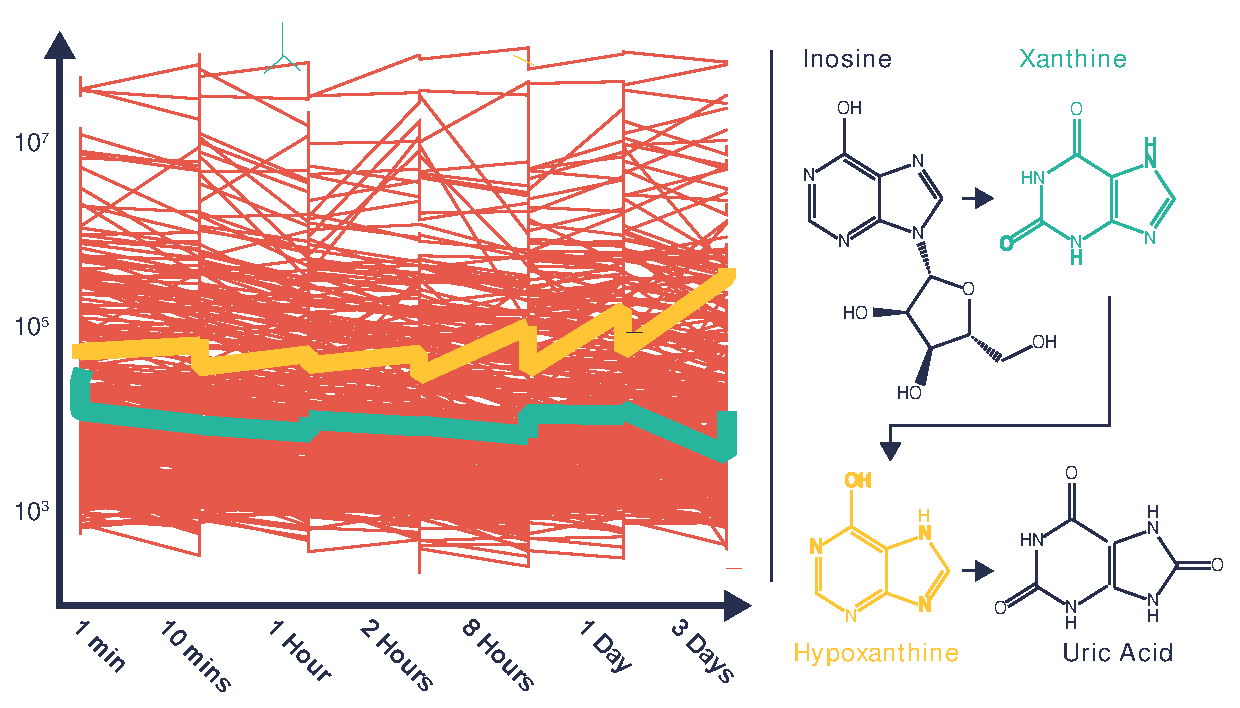
\includegraphics[width=1.2\linewidth]{2.Optimizaiton_Figures/Extraction_Details.pdf}}
		\caption{\textbf{Left} Time series intensities of all metabolites detected in pilot study 2 at different time intervals. In \textbf{yellow}, intensities for Hypoxanthine, a thermal degradation product of Xanthine can be seen increasing with time and in \textbf{green} the intensities of Xanthine is decreasing with respect to time due to thermal degradation  \textbf{Right} Thermal Degradation pathway of Inosine to Uric acid as described in \citep{FangThermalInvestigation}  }
		\label{fig:Pilot Study 2 - Extraction Time Series}
	\end{figure}
	
	The results from the times series extraction experiment are shown in the figure \ref{fig:Pilot Study 2 - Extraction Time Series}. Individual traces from the extraction data can be found in Appendix \ref{appendix: Extraction Kinetics Traces}. Although metabolite extraction results appear chaotic and randomly varying through multiple magnitudes of ion intensity, there is only a 1.2\%-8.7\% time-dependent increase between 10 mins and 1 day extraction times. Irrespective of molecule types, the 1 min extraction shows the largest CVs across the samples. This is to be expected as 1 minute is too short a time for a quantitative extraction. Accordingly the coefficients of variation decrease between the 1 hour and 1-day extractions from 22\% to 16\% however, the CV rise again in the 3 day extraction to 23\%. Is this due to the accumulation of known thermal degradation production. Inosine is thermally decomposed to uric acid through Xanthine and Hypoxanthine intermediates \citep{FangThermalInvestigation}. In the data, Xanthine decreases from an average intensity of $3\times10^4$ to $8.8\times10^3$ and concomitant increases in hypoxanthine from $7\times10^4$ to $2.3\times10^5$ from the 1 day to 3 days can be seen.
	
	As a result, the 1-day extraction time is kept as the extraction time moving forward as it allows for a full day sample extraction on the followed by a full day of downstream preparation on the second. Moreover, the Hypoxanthine to Xanthine ratio alongside other known degradation pathways of amino-acids \citep{Anton2015PreAnalytical} found in our data can now also we used as a loose proxy to diagnose the degradation state of a sample.
	
	\subsection*{Effect of Freeze-Thaw}
	
    Freeze-thaw cycles can be detrimental to sensitive biological samples such as proteomic sample preparations enriching for post-translational modifications \citep{Paltiel2008}. Although metabolites are small molecules it was not obvious whether the formation of water crystals that puncture cell membranes and damage protein has no effect on metabolites. Another motivation for investigating what happens to the sample when frozen is, that if there is no detected effect, samples can be freeze-dried rather than evaporated in a heated vacuum centrifuge before long-term storage.
	
\begin{figure}[th]
	\makebox[\textwidth][c]{
	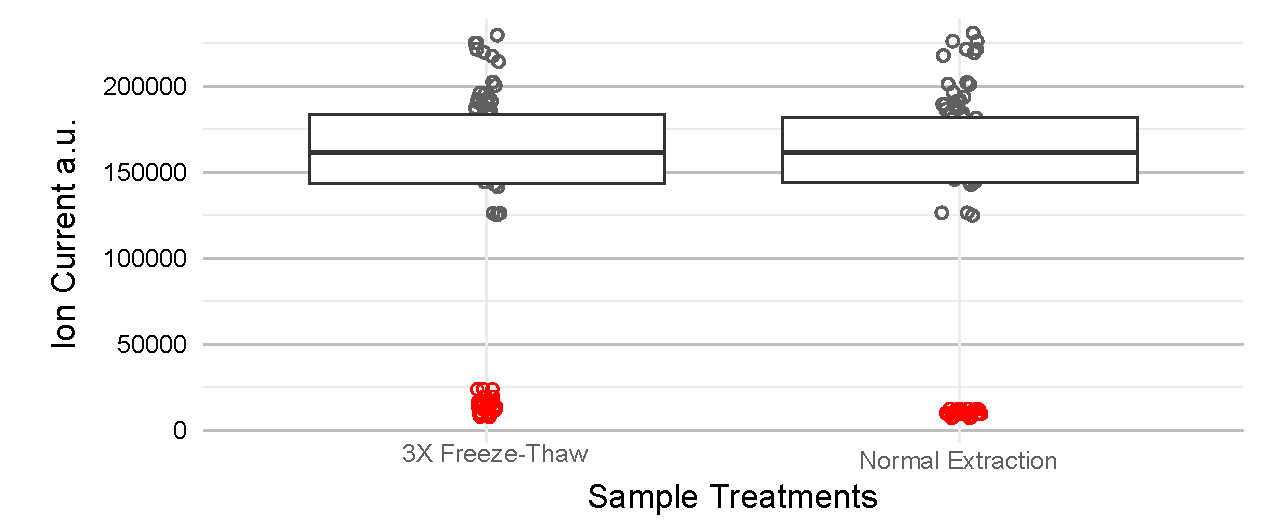
\includegraphics[width=1.2\linewidth]{2.Optimizaiton_Figures/Freeze_Thaw}}
	\caption{The effect of 3 freeze-thaw cycles on metabolites. Rep 1 samples were extracted for 1 day using the cold extraction protocol. Rep 2 samples were also extracted using the 1 day cold extraction protocol but also frozen and allowed to thaw 3 times}
	\label{Boxplots: Effects of Freeze Thaw Cycle}
\end{figure}
	
    Figure \ref{Boxplots: Effects of Freeze Thaw Cycle} shows the results from 3 freeze-thaw cycles on metabolites profiles. Four mouse liver extracts suspended in water were placed in a -20$^\circ$C dry ice \ch{H2O:EtOH} solution for freezing and thawing at 4$^\circ$ in the fridge three times. The differences between the two cohorts of metabolites are not significantly different (p-value 0.89), thus verifying the previously held hypothesis that the small molecules extracted in this experiment are not affected by the freeze-thaw cycles. A minority of molecules, including benzene, ETOH and MeOH were found in trace amount in the samples that were frozen, as seen from the outliers highlighted in red. There are thought to have come from impurities from splashing reagents during sample transfer.
	
	\subsection*{Quantification of Cross-Contamination }
	
	In the first pilot study, one of the HF mice showed unusually high levels of metabolites such as N6-MethylLysine which are normally only enriched in CD mice, due to cross contamination. In the previous pilot study, there was only one blank (ultra pure water) well for all of the samples on the plates. The total ion intensities for that mouse were lower compared to the other samples and so the relative effects of cross contamination were magnified. 
	
	In order to prevent this, two wells of millipore water are added for every row of 10 samples on the 96 well plate. Figure \ref{fig:TIC of Mouse Metabolties and Blanks} shows the intensities of 100 metabolites colored by strain on the top and the same metabolites, plotted for the blank samples. From this plot one can determine that on average the blank wells, even with many interspersed through out the plate have 2-5\% of the liver samples due to cross contamination in the sample loading capillary. Thus 4-10\%, two times the intensity of the metabolites seen in the "blank" wells is the inherent limit of discrimination between two samples. As a result minute fold changes cannot be differentiated from contamination precluding analysis of many reaction ratios that are regulated very close to equilibrium at equal concentrations close to the signal intensity baseline \citep{VanEunen2010,Traut1994,Beard2002,Schellenberger2010}.
	
\begin{figure}[hbt!]
	\makebox[\textwidth][c]{
	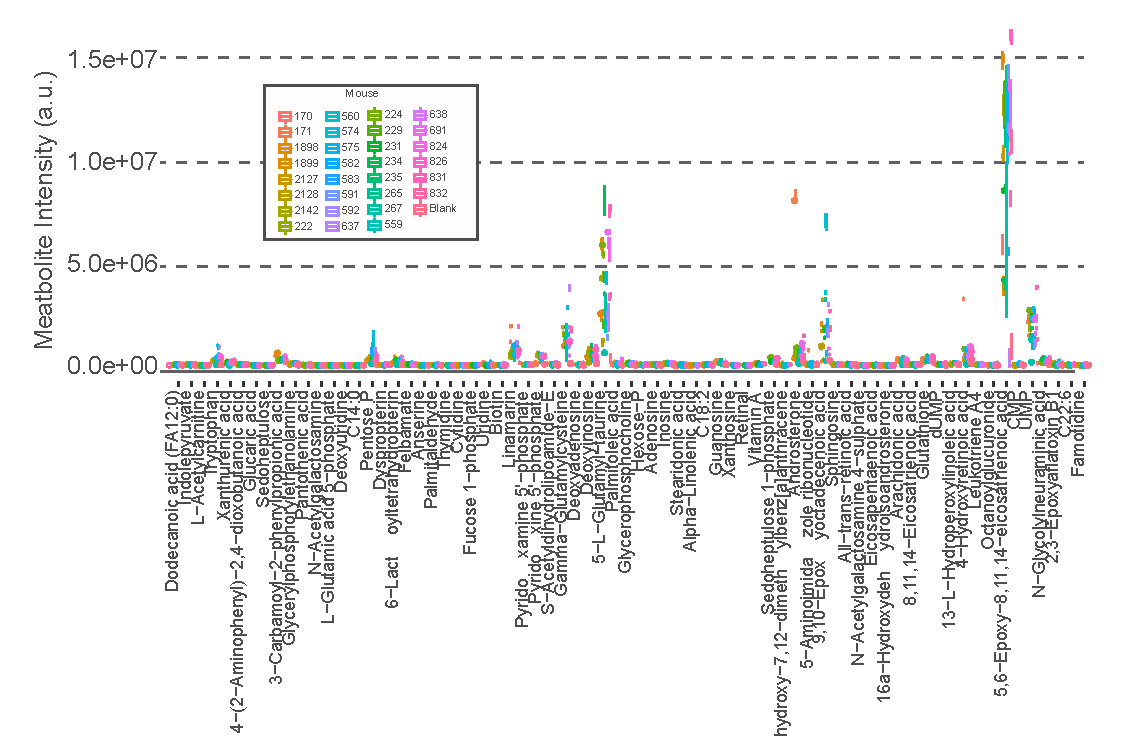
\includegraphics[width=1.2\linewidth]{2.Optimizaiton_Figures/TIC_All_Mice_Final}}
	\makebox[\textwidth][c]{
	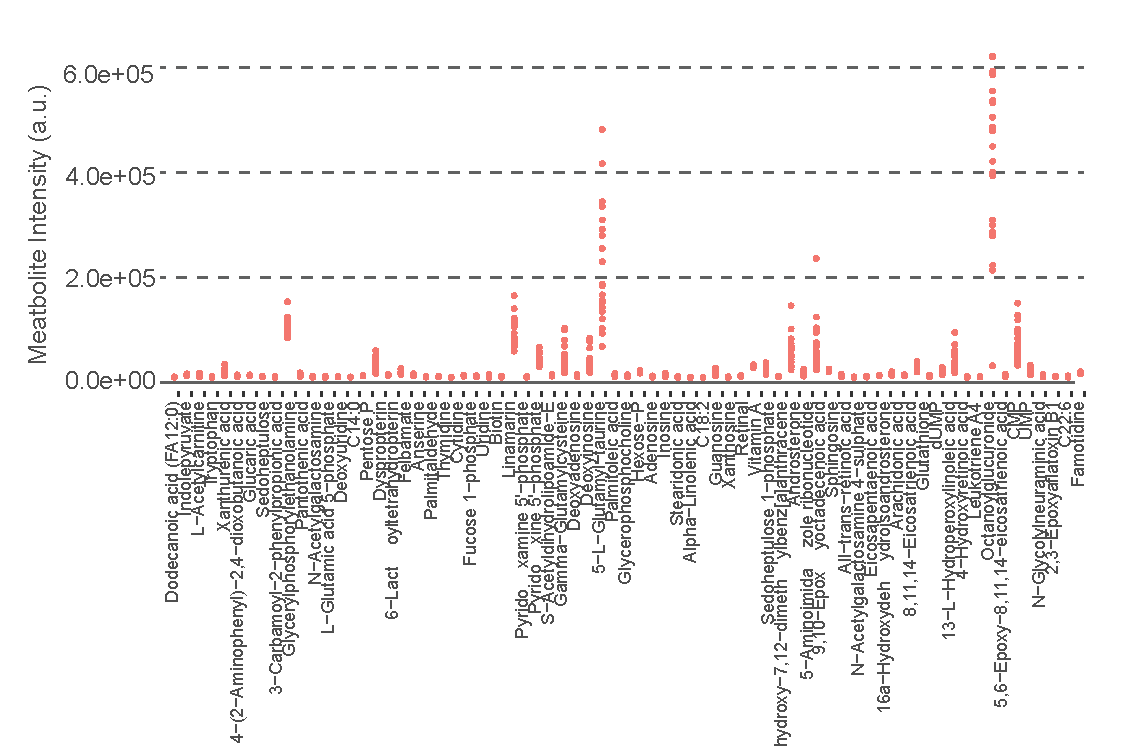
\includegraphics[width=1.2\linewidth]{2.Optimizaiton_Figures/TIC_Blank_Final}}
	\caption{\textbf{Top:} Metabolite Intensities from all the mice in the second pilot study \\ \textbf{Bottom:} Metabolite intensities from all of the wells that were only filled with water}
	\label{fig:TIC of Mouse Metabolties and Blanks}
\end{figure}
	
	
	
	\subsection*{Conclusions from Pilot Studies}
	
	At the end of the protocol optimization, the 24 hour cold extraction was determined to be the best option for the full run of 631 samples because a large number of metabolites could be quantified at high intensity and the extraction would be easy to plan around. Even if the sample were not extracted at exactly 24 hours, the relative effect of time on the sample intensities is reduced between 8 hours and 24 hours as compared to 10 minutes and 1 hour extraction time regimes where timing is more crucial. We found out the effect of secondary, homogenization was minimal, similar to the effect of freeze-cycles on the metabolites. Unfortunately a large cross-over contamination between samples was also discovered. Once the protocol was optimization the full run with all 631 samples were done. The methods of extracting and aligning the metabolites features from the mass spectra of all 631 samples is detailed in next section.
	
	\clearpage
	\section{Metabolite Data Acquisition and Handling}
	
	The two categories of data processing for metabolomics can be divided into the processing the raw intensity data from the mass spectrometer and high level analysis ,interpretation and contextualizing of the data in biological networks. Raw data generated by the mass spectrometer is processed using a Matlab script called FIAminer which takes the peaks from the raw profiles and outputs a csv matrix file containing all of the samples, metadata and metabolite annotations (Zamboni, Unpublished). The data analysis and interpretation is done in R in addition to the use of KEGG \citep{Kanehisa2017} and MetaboAnalyst\citep{Xia2016UsingAnalysis} for pathway analysis.
	
	\subsection{Raw Data Acquisition and Processing}
	
    The TOF-MS used in this study is the 6550 Quadrupole Time-of-Flight, shown in the figure \ref{fig:A schematic of the 6550 Time-of-flight Mass spectrometer}. Complex metabolite solutions are electro-sprayed into the mass spectrometer without any liquid chromatography. Next, this ion gas traverses a small lateral distance through a quadrupole drift tube and enter into a large time of flight mass analyzer that projects out of the top of the machine. The raw intensities that are generated by the mass spectrometer in a study are a continuous sampling of the detector current at regular intervals. Once ions flying through the mass analyzer hit the detector surface \citep{Glish2003TheCentury}, they cause a cascade of electrons that spread in a wave propagating on the detector surface, which is seen as a peak in the ion current. This current when it is plotted continuously is known as the raw profile. The raw profiles from three different samples with multiples replicate can be seen in the bottom panels of figure \ref{Raw Metabolite Profiles}. 
	
	\begin{figure}[hbt!]
		\centering
		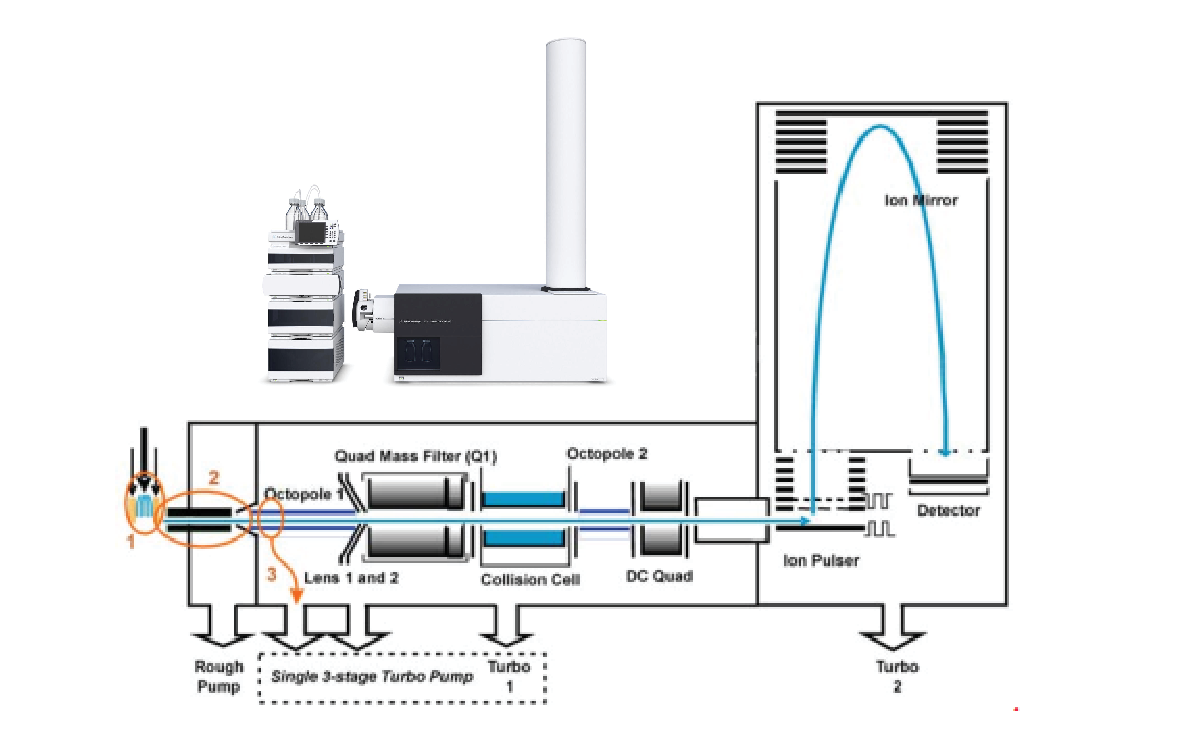
\includegraphics[width=\linewidth]{3.Metabolomics/MS.pdf}
		\caption{Adapted from \citep{AgilentTechnologies2017} of the 6500 TOF-MS with an included schematic of the flight path. The blue line int he schematic represents the path of the ion after they are softly ionized and electro sprayed into the instrument }
		\label{fig:A schematic of the 6550 Time-of-flight Mass spectrometer}
	\end{figure}
	
    Similar to optical instrumentation where lines may broaden with an incorrect optical arrangement and lens degradations, the widening of the peak shape in the profiles data is due to the dispersion of the ion packet or aberrations from stray electric fields in the mass spectrometer\citep{Glish2003TheCentury}. Along the flight path of the mass analyzer, many factors may lead to the broadening of a packet of metabolites flying towards the detector which must be considered for accurately determining a baseline intensity and centroiding the profile data. In TOF-MS instruments used in this experiment, the peak shapes show fast intensity spike with a gradual decay of the signal (figure \ref{Raw Metabolite Profiles}.C). This is due to the arrival of highly abundant isotopically pure and lighter ions arriving at the detector first, followed by heavier isomers lower abundance ions.
	
    The shape of the peaks in the profile generated by an instrument is a function of the sum of conditions and voltages on all of the ion optics and is known as the MS Tune. In the figure below, well-defined peaks can be seen in the lower M/Z range highlighted in the boxes on the left side of the figure. The peaks are strong and can be easily aligned and averaged across all the samples and extracted in an automated manner using FIAminer. However, the signals in the high m/z regime is much lower intensity as seen in the centroided spectra shown in figure 2.1.A, and requires a high resolving power instrument to detect distinct peaks in the convoluted grass. Through a comprehensive calibration process in that involves not just m/z, as is the case for all conventional MS calibration, but also the peak shape, these smaller peak features can be extracted (Zamboni, Unpublished). 
	
	\begin{figure}[hb!t]
		\makebox[\textwidth][c]{
		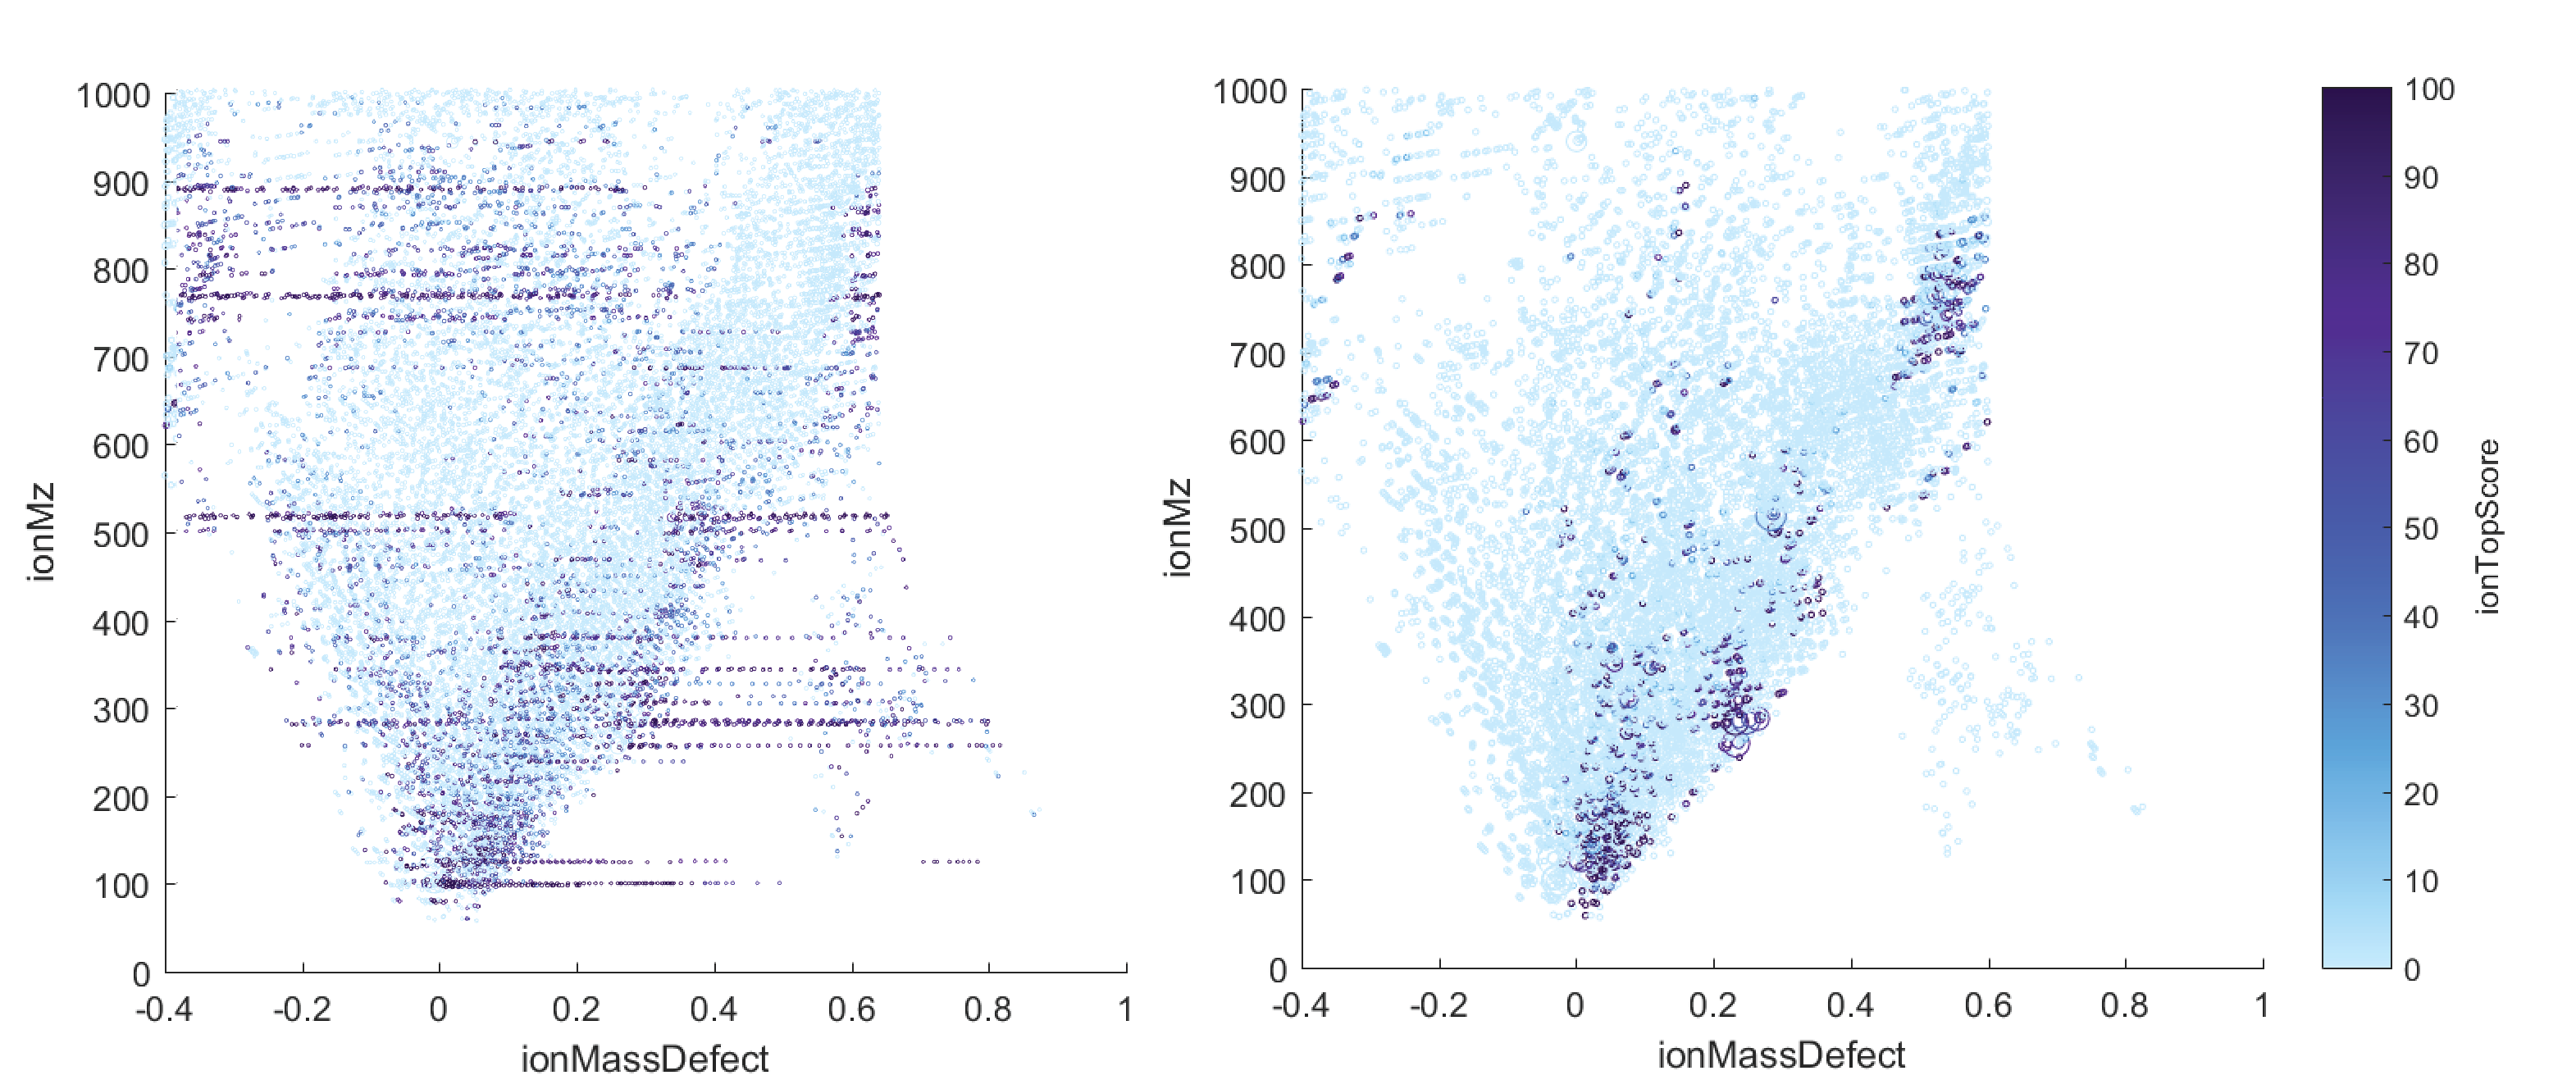
\includegraphics[width=1.2\linewidth]{3.Metabolomics/Peak_filtering.png}}
		{\caption{Left: All annotated peak annotated automatically. Right: Ringing peaks and impossible mass combination filtered}}
		\label{Metabolomics Data Pre-Processing}
	\end{figure}

	A final processing step removes artifacts that appear during the analog to digital signal conversion detector in which pre-amplifier electronic noise is recorded and appears as horizontal streaks in the figure above. These is known as ringing peaks\citep{Goodner1998QuantitationSpectrometry}. Since they show up at m/z ratios that cannot be attributed to any sum of know elements or isotopic mixes, they are easily removed.
	
	During the course of this peak assignment, each peak assignments is given a score and only perfect score peaks are used in the final analysis. In an average sample analysis 19 000 featured were detected, 1500 of which could be annotated with some certainty when searched against the HMDB \citep{Wishart2013HMDB2013}, Metlin\citep{Smith2005METLIN} and KEGG databases\citep{Kanehisa2017}. The majority of detected features however cannot be annotated and are cryptically known as dark matter in the mass-spectrometry community \citep{Aksenov2017GlobalSpectrometry}.
	
	\begin{figure}[htb!]
		\makebox[\textwidth][c]{
		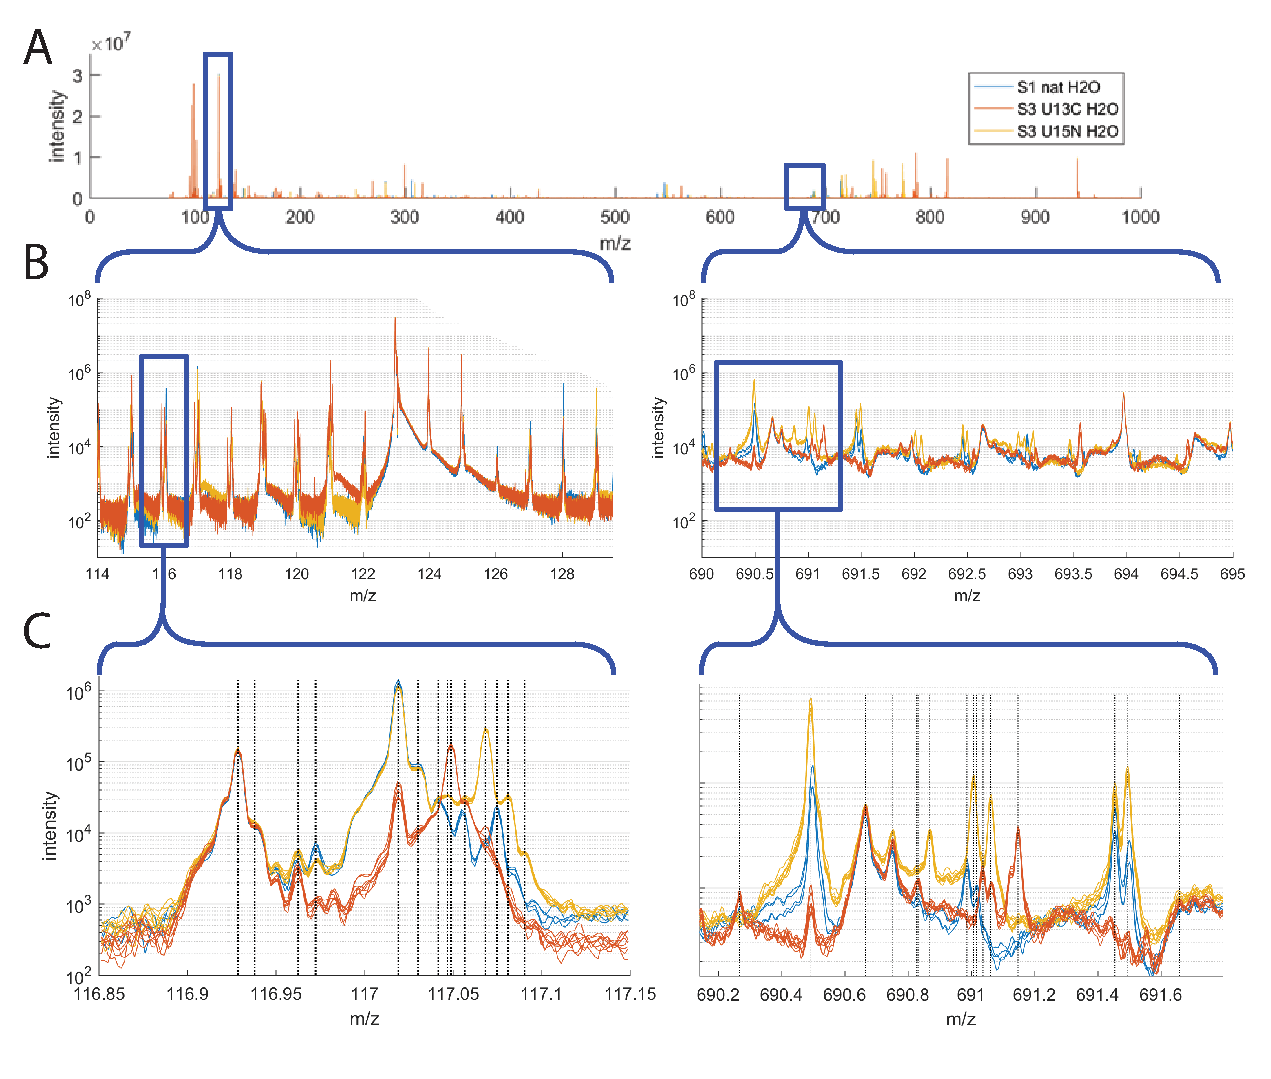
\includegraphics[width=1.2\linewidth]{3.Metabolomics/Raw_Signal.pdf}}
		\caption{A. Centroid level data for the metabolite peaks from [0,1000] m/z\newline    
			B. A zoomed-in view of the lower mass range around 100 m/z. The peaks in the lower mass range are well defined and can be fitted with the mixture a mixture of Gaussians to determine their maximum values. high m/z range peaks which are less well defined and required an additional operation to stabilize the baseline before peaks can be centroided.
			C. A further zoom into the spectra again shows the unstable characteristic of metabolites peaks in the high m/z ranges which pose a challenge to process in an automated manner.}
		\label{Raw Metabolite Profiles}
	\end{figure}
	
	\section{Data Analysis}
	
	\subsection{Normalization of Metabolite Data} 
	
    In metabolomics, the physiochemical property range of the molecules is sufficiently large such that a small subset of metabolites, analogous to spike-in peptides at known concentrations in proteomics, cannot be used as an internal control for intensity normalization \citep{Valikangas2016}. This is because the intensity of a molecule is not a simple linear function of the metabolites concentration, but rather a convolution of ionization efficiency, fly-ability and voltages biases on the electronics in the mass spectrometer. Thus the only factor we can normalize the metabolites to are the originally weighed masses of the liver tissues, the metabolites were extracted from \citep{Valikangas2016}. This normalization, although crude yields highly normal data allowing us to perform statistical tests without breaking the normality assumption.
	
	\begin{figure}[ht!b]
		\centering
		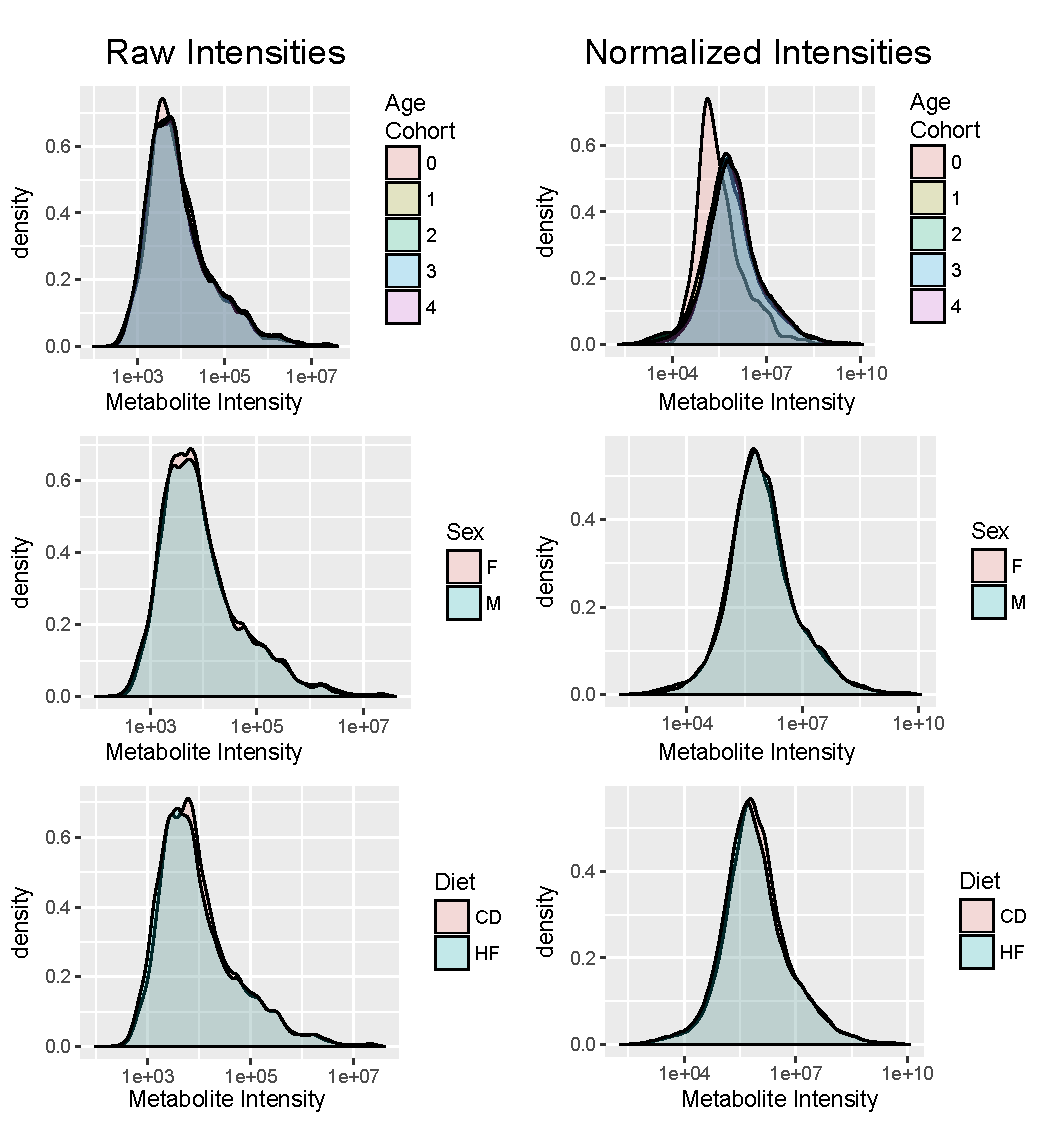
\includegraphics[width=\linewidth]{3.Metabolomics/Factor_Densities_Final.pdf}
		\caption{Metabolites intensities normalized to the amount of tissue is extracted from show normalized even when segregated into separate groups}
		\label{fig: Meatbolite Data Normalization}
	\end{figure}
	
	\subsection{Quality Control}
	
    Once the data has been normalized, summary statistics of the full run data are generated. Firstly, a plot of the metabolite intensities overlaid over a map of all of the reaction in the metabolism of mice is used to show the metabolome coverage. The map of the coverage can be found in Appendix \ref{appendix:Metabolome Coverage}. In both of the full metabolome runs of 621 mice livers, all the major KEGG pathway categories except drug and xenobiotic metabolism are covered. This is a good sign as the controlled diets did not contain common drugs or xenobiotics. 
	
\begin{figure}[bht!]
		\centering
		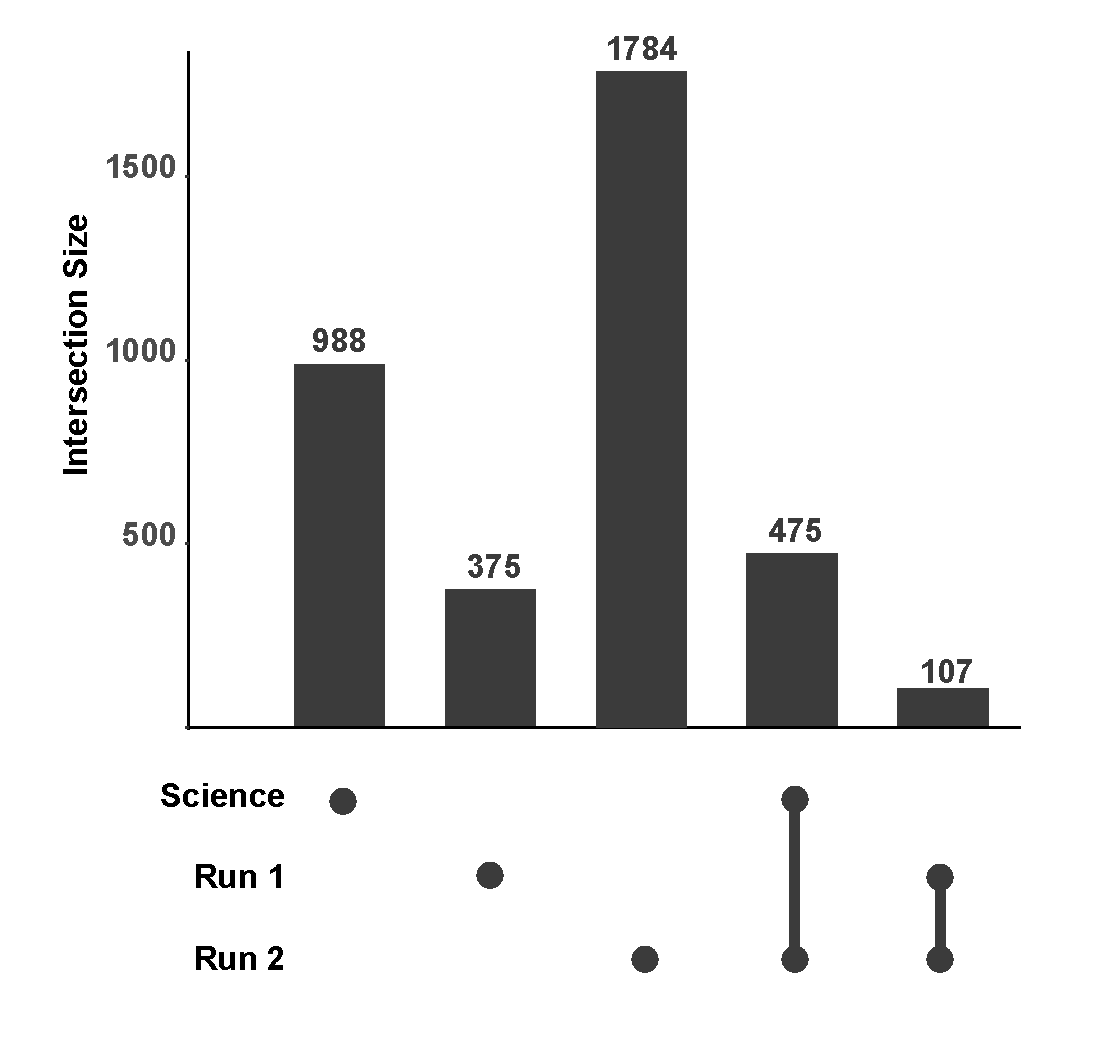
\includegraphics[width=0.7\linewidth]{3.Metabolomics/Metabolite_Set_Overlap}
		\caption{ Number of metabolite annotations in the previous Science paper by \citeauthor{Williams2016SystemsFunction}, and two full metabolome experiments conducted for this thesis. The second run, done with much higher care and attention to timing and temperatures during the preparation yields a much higher number of hits.}
		\label{fig:Unique Metabolite Annotations}
\end{figure}

The number of metabolites in the first full run performed on all 621 mouse livers samples disappointingly yielded only a third of the metabolites annotations as compared to the Science paper. This was due to the logistical challenges of dealing with this many samples and issue with refrigerators containing the samples losing power, allowing them to heat up before analysis. Fortunately, the second run of all the metabolites was performed with improved planning and backup refrigerators. A much higher number of annotations could be made, with 475 metabolites overlapping with the science paper, giving us a large set of data to cross-validate conclusions.

To get a summary view of ion intensities, the average total ion counts of the metabolites in the mouse and the blank samples are plotted together in figure \ref{fig:Total Ion Counts}. Here only the data from the first full run is shown. As seen previously, the mass spectrometer has a very large dynamic range and detects metabolites in over 4 orders of magnitudes. The on average the signal from the blanks is 2 order of magnitude smaller and cross-contamination signal in the full runs is only 2\%-3\% of the signal.
	
\begin{figure}[hbt!]
	\makebox[\textwidth][c]{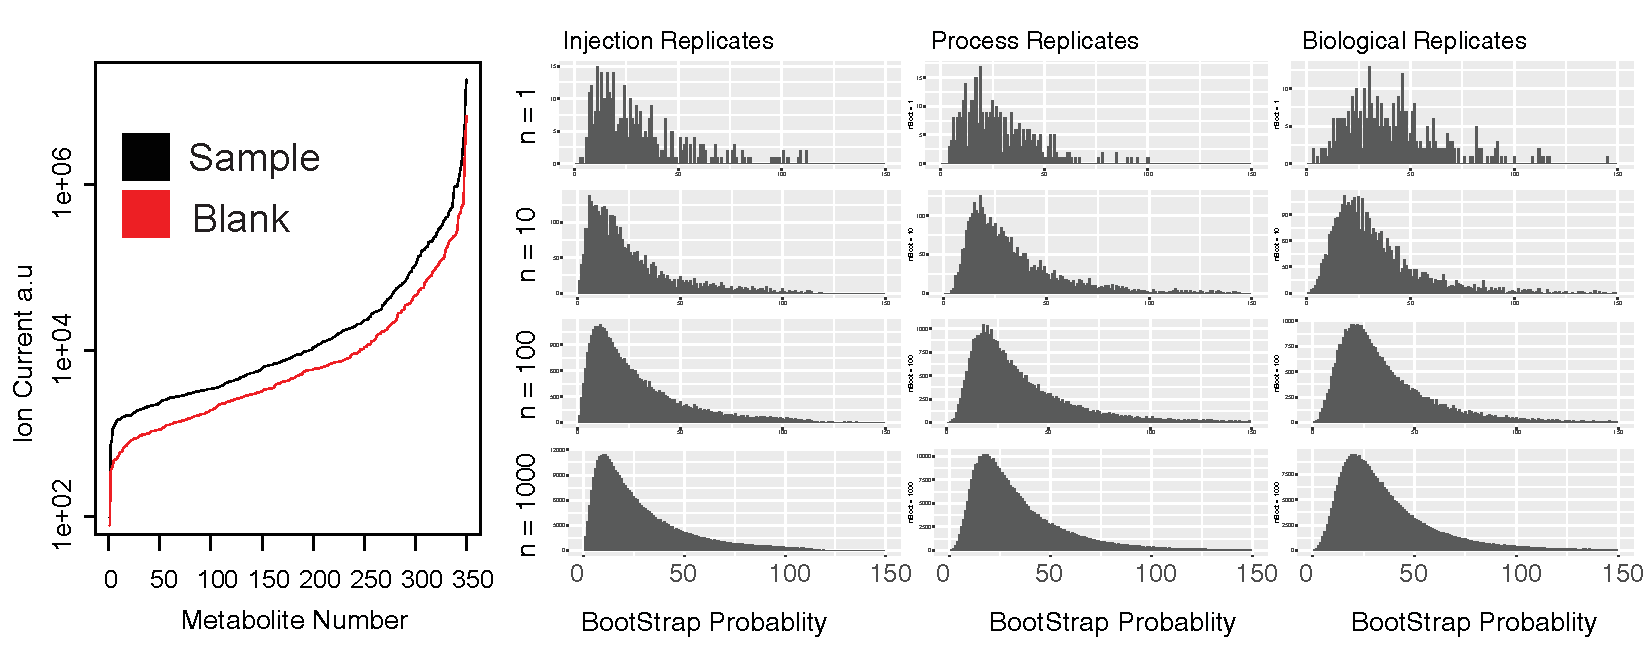
\includegraphics[width=1.3\textwidth]{3.Metabolomics/CV_TIC.pdf}}%
	\caption{\textbf{Left:} The Ion intensities of different metabolites plotted from lowest to highest in the mouse samples (in black) and in the black well (in red) that had only water. The signal from the blanks is the result of cross-contamination.\textbf{Right:} Bootstrap CV calculations of injection replicates, process replicates and biological replicates}
	\label{fig:Total Ion Counts}
\end{figure}
	
A bootstrapping sub-sampling method is used to generate the coefficient of variance(CV) between, injection replicates (samples that are sequentially injected one after the other), process replicates( samples that come from the same mouse liver and are extracted using the same protocol) and biological replicates (samples that come from two different mice that are the same strain and within the same diet and age cohort). The bootstrap distribution of the injection replicates has the lower CV with a mean of 7\% and a sharply defined mean. The process replicates and biological replicates have a slightly higher CVs at 8\% and 12\% which is within the precision of metabolomics in the previous paper, but slightly on the higher side. These CV values are replicated in both runs on the mouse livers samples but lower in the second full run.
	
	\begin{figure}[bh!t]
		\centering
		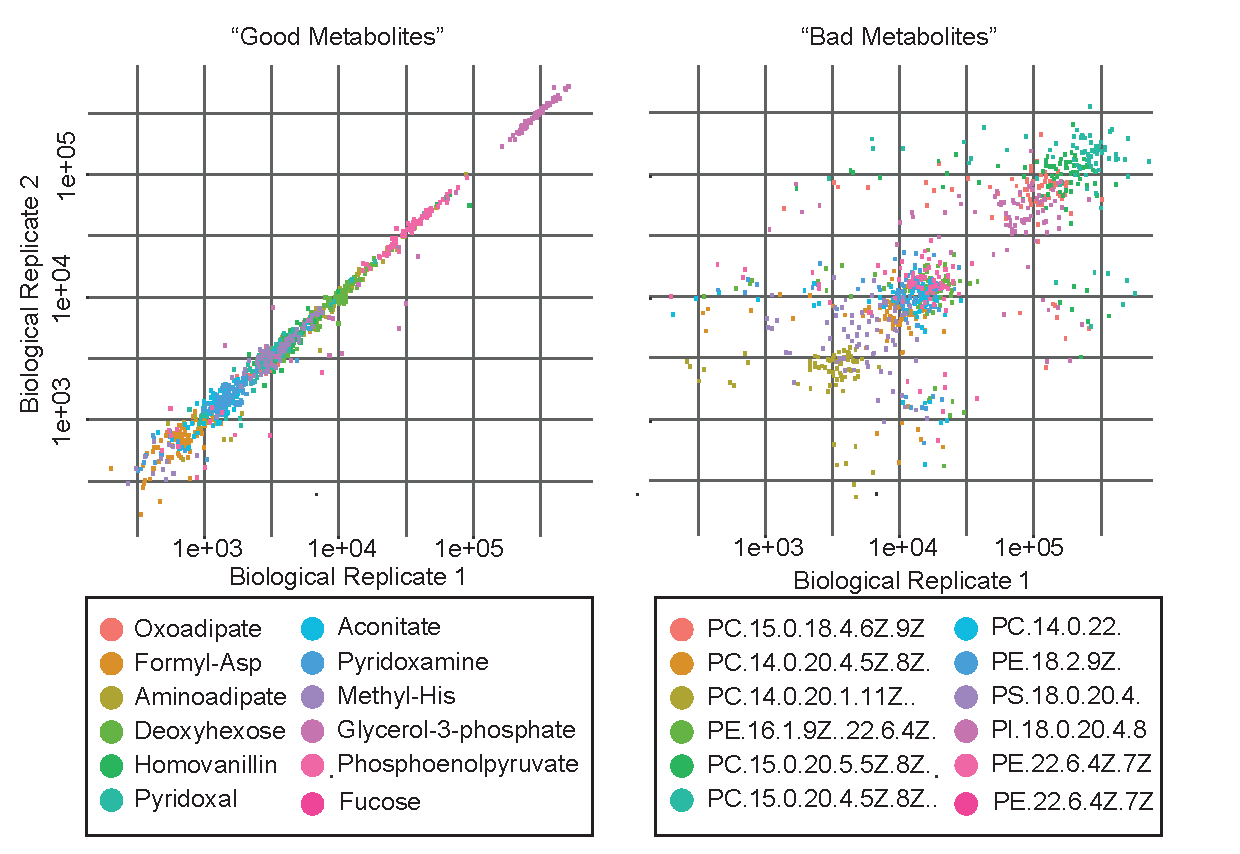
\includegraphics[width=\linewidth]{3.Metabolomics/Good_and_Bad_Metabolites.pdf}
		\caption{ \textbf{left} Small polar molecules are extracted effectively form the liver samples and correlate strongly within biological replicates. \textbf{Right} Non-polar molecules are not well extracted using the extraction protocol this method and are unreliably extracted] }
		\label{Fig:Good and Bad Metabs}
	\end{figure}
	
    Most high CVs are the result of metabolites that are not quantitatively extracted with the small polar molecule extraction protocol. Figure \ref{Fig:Good and Bad Metabs}  shows the two classes of metabolites and their correlations between biological replicates. Small polar molecules such as oxoadipate and aconitate, are quantitatively extracted and show a robust correlation between biological replicates. Phospholipids, ceramides, cholesterols, and prostaglandins often are not well extracted using this protocol and have high CVs between biological replicates. In addition to being poor measurements, the chemical reaction that catalyzes the anabolism and catabolism of these lipid molecules are often cyclical, a single enzyme may oxidize fatty acids of multiple lengths. This complicates QTL analysis and does not allow us to pick a single affected enzyme, reactant, product trio in our network analysis. It is for these two reasons the fatty acids are excluded from QTL analysis.

	Clustering is the last method used to quality control the shape of the data. Manhattan hierarchical clustering and Mankowski clustering is used. Ideally, injection replicates, bio-replicates and diet cohorts should cluster together, rather than samples that were extracted in the same batch being clustered together, indicating large batch effects. Hierarchical clustering, k-means and PAM based methods on the raw data may not be sensible when the variables are measured in many orders of magnitudes. Metabolites with the largest ranges get the most weight and might dominate the analysis. As such, the variables can be are scaled and the standard intensities are used for the clustering analysis.

	In figure \ref{fig:Clustering Analysis} all the samples from Mouse 1481 are clustered together (shown in pink). In orange, all of the replicates for mouse 1270 are clusters together, however, there is a single run that had an error in the injection that is clustered with another mouse strain.  The many biological replicates of C57BL/6J mice are all clustered with their injection replicates, however, the Minkowski distance is much for effective at ascribing these samples to a single cluster. Except for the 1 mouse in this subset, all the other mice are clustered with their injection replicates. Both the Manhattan and Minkowski distances yield the smallest averages distances between, injection replicates, strains, and diets respectively. The clusters of samples in different age cohorts are robustly determined, indicating the metabolites that differ between age cohorts of mice a do not show stark dichotomies as the metabolites that differ between the diet cohorts. As a results age, mice in the same age cohort on ages may not be clustered together using either metric. The cluster analysis yields a satisfactory result, and there is confidence in the data. Thus, more biologically orientated questions can be asked. 
	
	\begin{figure}[hbt!]
		\makebox[\textwidth][c]{ 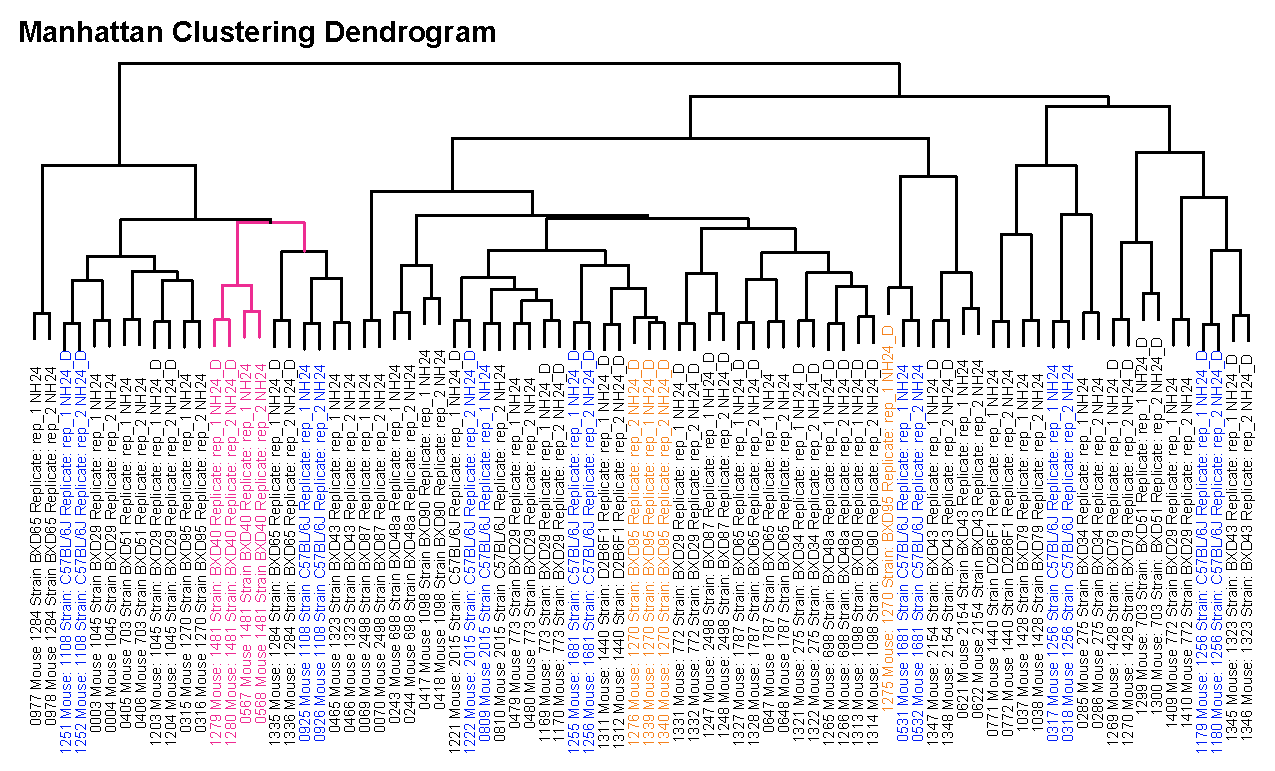
\includegraphics[width=.6\linewidth]{5.Clustering_Results/Clustering_Results_1_Done.pdf} 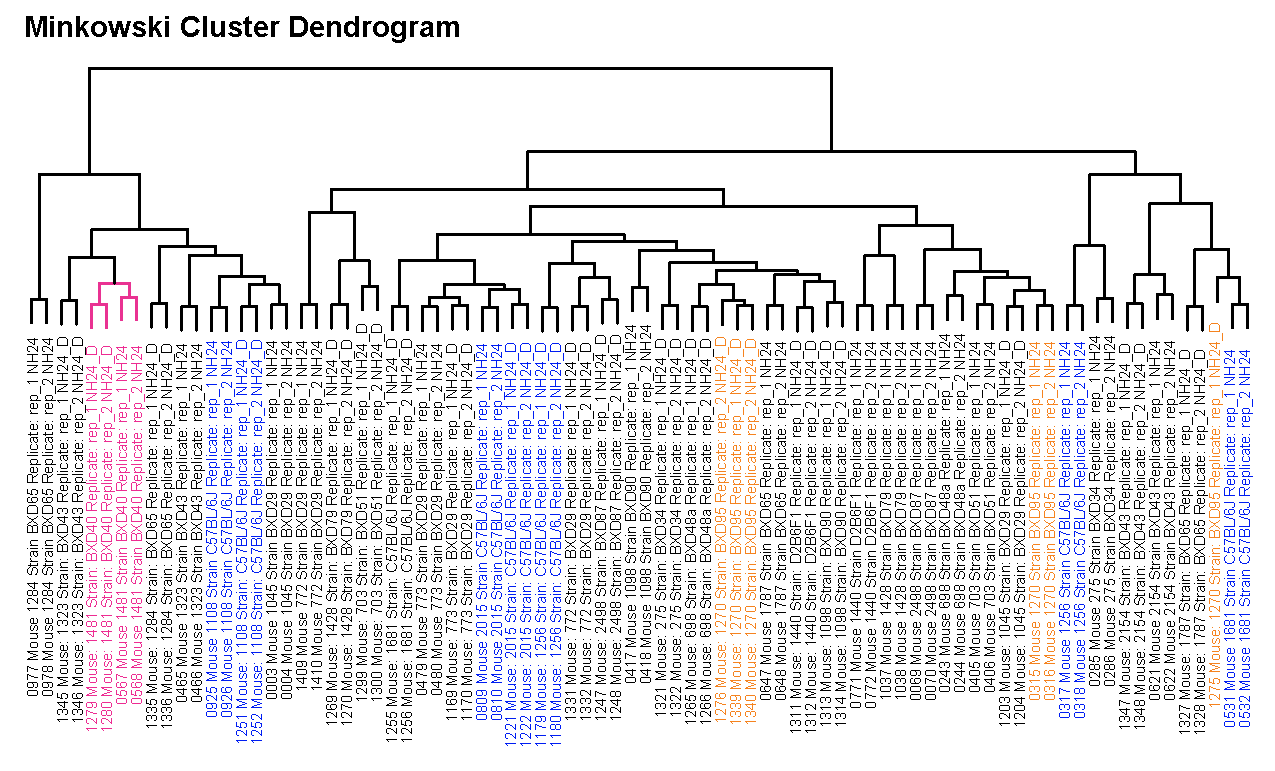
\includegraphics[width=.6\linewidth]{5.Clustering_Results/Clustering_Results_6_Final.pdf}}
		\caption{ \textbf{Top:} Hierarchical agglomerative clustering using Manhattan distances. Below: Hierarchical cluster performed using the Minkowski distance which is more robust to noise. Biological and injection replicates are colored to qualitative assessment of the clustering result}
		\label{fig:Clustering Analysis}
	\end{figure}
	
	
	\section{Analysis of Metabolic Data}
	
	\subsection{Metabolite Fold Changes}
	
    The purpose of performing this extensive metabolomic search to identify differences in the metabolomes of mice in different diet and age cohort. Metabolites that were robustly different between the HF and CD mice in the previous metabolic colony experiments are observed again in aging the colony but show lower fold change ratios and intensities. In the volcano plot (figure \ref{volcano: Meatbolite Fold Changes}) on the left, allyl isothiocyanate, allysine, 2-oxoadipate, and fucose are among a large group of metabolites that have large fold changes in mice that are on a chow and high-fat diet. 

	The volcano plot for metabolites with significant fold-changes between old and young mice 2-oxoaditpate and fucose also accumulate in higher quantities in older mouse livers in addition to bilirubin and taurocholic acid derivatives. However, taurocholic acid is a cholesterol derivative and cannot be trusted to be reproducibility measurable. Molecules like bilirubin which are markers for jaundice can also be an interesting target because of the fact that as mice age, they seem to have a reduced ability to remove bilirubin from their livers. The physiological function and reason why these metabolites make good metabolic disease markers are given below.
		
	\begin{figure}[t!]
		\makebox[\textwidth][c]{
		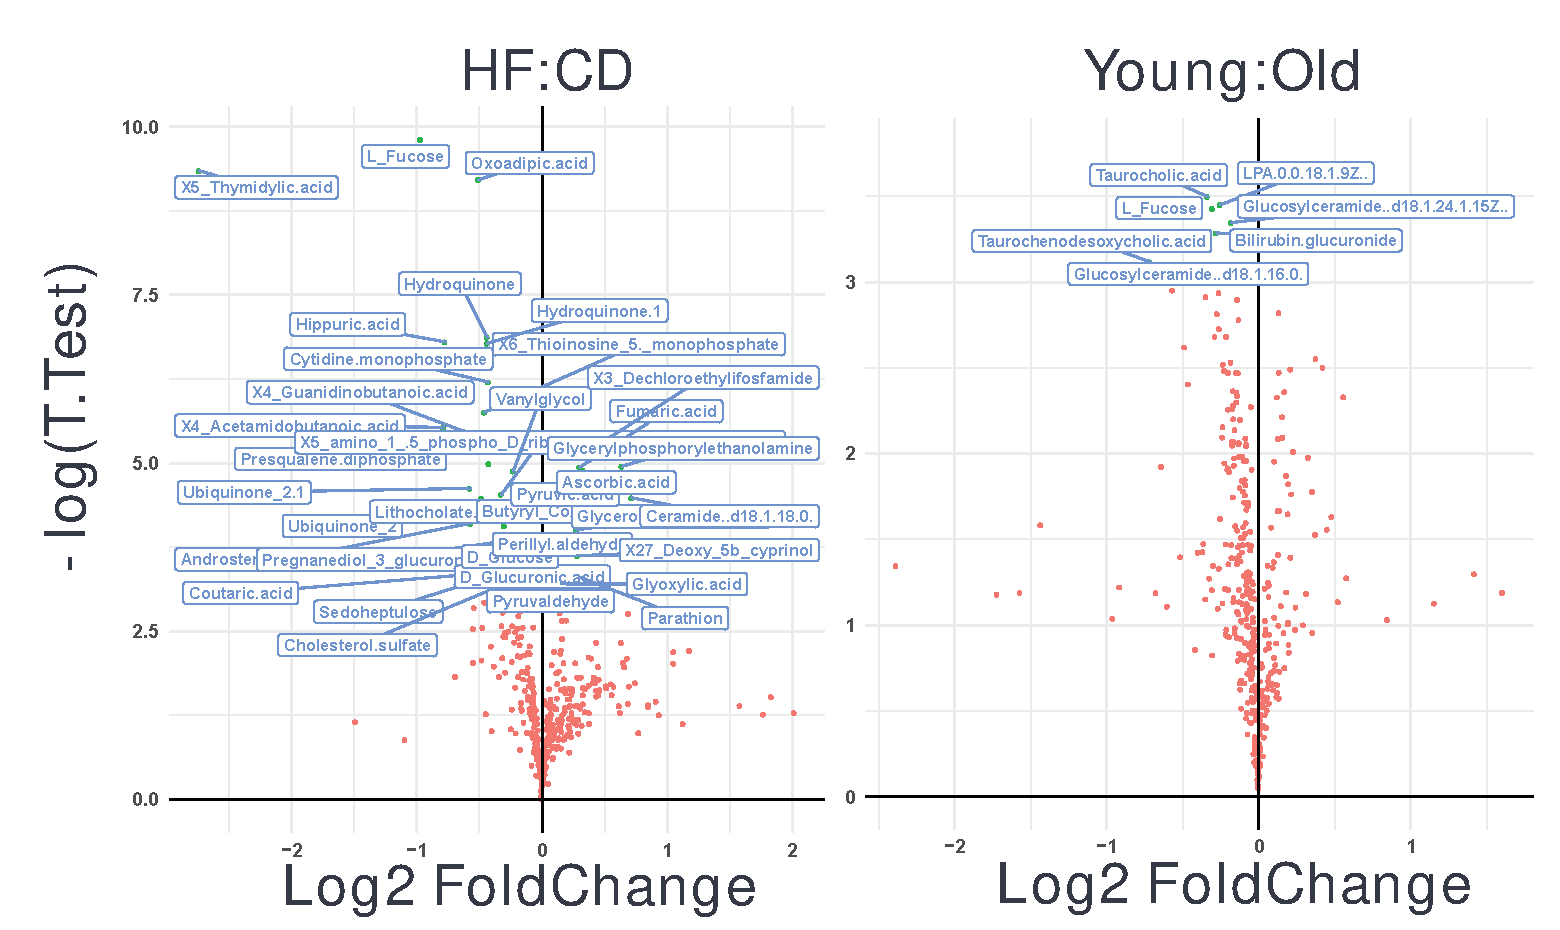
\includegraphics[width=1.1\linewidth]{3.Metabolomics/Volcano}}
		\caption{Volcano Plot of the fold changes between mice in different diets cohorts on the left and mice in different age cohorts on the right. The significance threshold is chosen at a t-statistic of 3 and an absolute log2 fold-change of 1}
		\label{volcano: Meatbolite Fold Changes}
	\end{figure}
	
    \textbf{AllyIsothiocyanate:}
	AllyIsothiocyanate accumulates in the chow diet mice in both the old metabolic colony from \citep{Williams2016SystemsFunction} and current aging colony mice. AllyIsothiocyanate(AITC) is found in high quantities in cruciferous vegetables and is highly bioavailable once digested \citep{Zlatkis1971ProfileUrine.} It is a secondary metabolite produced in high quantities in certain plants like horseradish and mustard but can be found in a large range of vegetables that may be present in the chow diet. AITC also has a very strong QTL, however, the QTL region is sparse in terms of SNPs and genes, containing many Riken genes which do not allow us to uncover the underlying affective loci conclusively. Although the stress-related regulation of AITC in plants is mechanistically understood, it is not likely its production is similarly regulated in mammals\citep{Kissen2016Allylisothiocyanate}.  

	\textbf{Aminoadipate \& 2-Oxoadipate:}
	Aminoadipate and 2-oxoadipate are both degradation products of lysine, tryptophan, and hydroxylysine produced in mammalian livers\citep{Higashino1965Saccharopine}. They are significantly enriched in HF diet mice and higher in older mice (p-value = 0.65). In humans, mutations in the Dehydrogenase E1 And Transketolase Domain Containing 1 (DHTKD1) leads to the accumulation of lysine and tryptophan degradation products and increases in detectable reactive oxygen species (ROS) \citep{Goncalves2016Production}. The DHTKD1 gene encodes a protein that catalyzes the conversion of 2-oxoadipate to glutaryl-CoA through a dehydrogenation reaction. The catalytic domain of DHTKD1 is structurally related to 2-oxoglutarate dehydrogenase and generates \ch{H2O2} and \ch{O2^-}, during oxidation of 2-oxoadipate which can cause age-related degradation and high-fat diet associated inflammation \citep{Goncalves2016Production}. 

	\textbf{Allysine:}
	Allysine is a product of lysine oxidation which is increased in the aging skin and diabetes patients that do not have renal failure \citep{Sell20072aminoadipic}.  In the maturation of fibular collagen in the skin LOX(Lysyl Oxidase),  oxidatively deaminates the lysine residue generating allysine. The interruption of this process can lead to the accumulation fo allysine and deterioration in the collagen matrix of the skin resulting in wrinkles \citep{Bailey1998Mechanisms}. Additionally,  the ϵ-amino group of lysine residues in proteins may undergo stochastic deamination by MCO (metal-catalyzed oxidation) reactions that produce allysine. This MCO catalyzed oxidation is also implicated in an age-related diseases such as  Alzheimer's disease and metabolic diseases such as atherosclerosis and diabetes \citep{Stadtman2004Role}. 

	\textbf{Fucose:}
	Fucose containing glycan is a post-translational modification on a range of serum proteins and is itself present at low concentration in the serum. Serum proteins are produced in the liver and aberrant fucosylation on these proteins are the result of mutations in the many fucosyltransferases\citep{Becker2003Fucose}. Proteins with incorrect fucose-containing glycoconjugates can create complications in a range of cellular processes and are a putative biomarker for many diseases including cancer, rheumatoid arthritis and diabetes \citep{Wiese1997Effect}. 
	
	After validating known HF and CD metabolites from \citep{Williams2016SystemsFunction} such as allysine and fucose, volcano plots of metabolites foldchanges between the two diet cohorts are used to determine a wider number of metabolites to perform QTL analysis with. The HF:CD volcano plot shows significant changes in central energy metabolism such as pyruvate, cMP, fumarate, and ubiquinone are enriched in the high-fat diet which may not be surprising. Pyruvate is also an intermediate in the ketone bodies pathway that is activated when there is low glucose but high fat in the blood serum. 
	
	D-glucose is also a significant hit and although it can be assumed glucose is the major isomer constituent of the peak, a targeted chromatographic separation assay would have to be optimized and implemented in order to resolve all the hexoses and determine this for certain. Additional carbohydrate metabolites such sedoheptulose are also an interesting trait. It also has many enantiomeric centers meaning this peak is mostly like a composite of all the c7 sugars in the pentose pathway. This pathway is interesting as it has implications for the rate of nucleotide synthesis which may be in pertinent in aging, however, the need for targeted mass-spectrometry to validate the hit is not appealing. What is largely missing from these metabolites which are enriched and depleted in HF are the amino acids. These metabolites are intermediates between the glycolytic and TCA cycle metabolites which one would assume would be hugely affected pathways with large diet based interventions.
	
\begin{figure}[t!]
		\makebox[\textwidth][c]{
		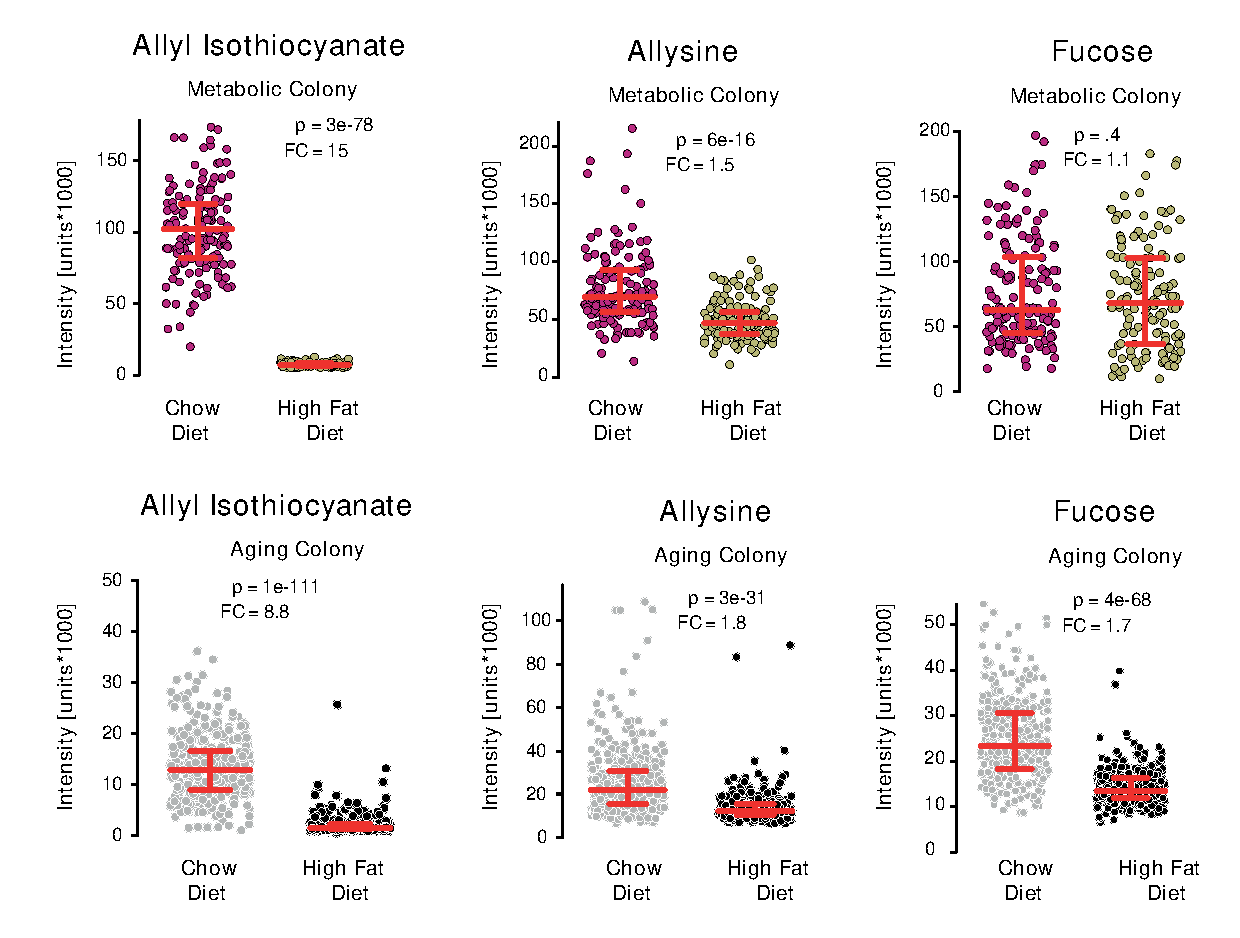
\includegraphics[width=1.1\linewidth]{3.Metabolomics/Top_3_Diet_Metabolites}}
		\caption{ Three metabolites, known to be highly enriched in mice on the HF diet are used as a positive control in this new mouse cohort. Allyl Isothiocyanate, allysine and fucose are all detected in the new mouse colony, however all three metabolites show weaker signal and smaller fold changes than those detected in the previous experiment by \citet{Williams2016SystemsFunction}}
		\label{fig:Top 3 Diet Metabolites}
\end{figure}
	

\section{QTL Analysis}
	
    The distribution of the raw QTL LOD scores for all of the metabolites with significant age related and diet fold changes are shown in figure \ref{fig: Distributions of QTL LOD scores for all significant Age and Diet related Metabolites}. In order to ensure the high scores were not simply generated by chance, the null distribution for the QTL LOD scores are computed. The genotyping array with which the QTL analysis is performed is scrambled after which the LOD score for the metabolites are recomputed. If the metabolite still shows an association with regions of the chromosome that has been completely scrambled, this means the association may have occurred by chance. A majority of the ‘real’ QTL have large overlapping segments with the LOD scores generated with the scrambled genotypes array indicating a need for a high LOD score threshold of 5-6 to be confident in a QTL. Thus, one should be careful in interpreting a QTL are causal if it exists in segments of the chromosome that has the proclivity to show high QTL LOG Scores even after scrambling. 
    
    One can see from this analysis that there are many significant metabolites QTLs that differ between diet cohorts. The top QTL results can be seen in Appendix \ref{fig:Metabolite QTL Results Tables}. On chromosome 3 of the QTL results, there is a range of significant QTLs that are manifest in the CD diet mice. The converse is true for chromosome 2 with mice on the high-fat diet. This speaks to the complex nature in which environment (diet) can allow the dissection of genetic drivers of certain phenotypic traits \citep{Abiola2003identification}.
	
	\begin{figure}
		\makebox[\textwidth][c]{
		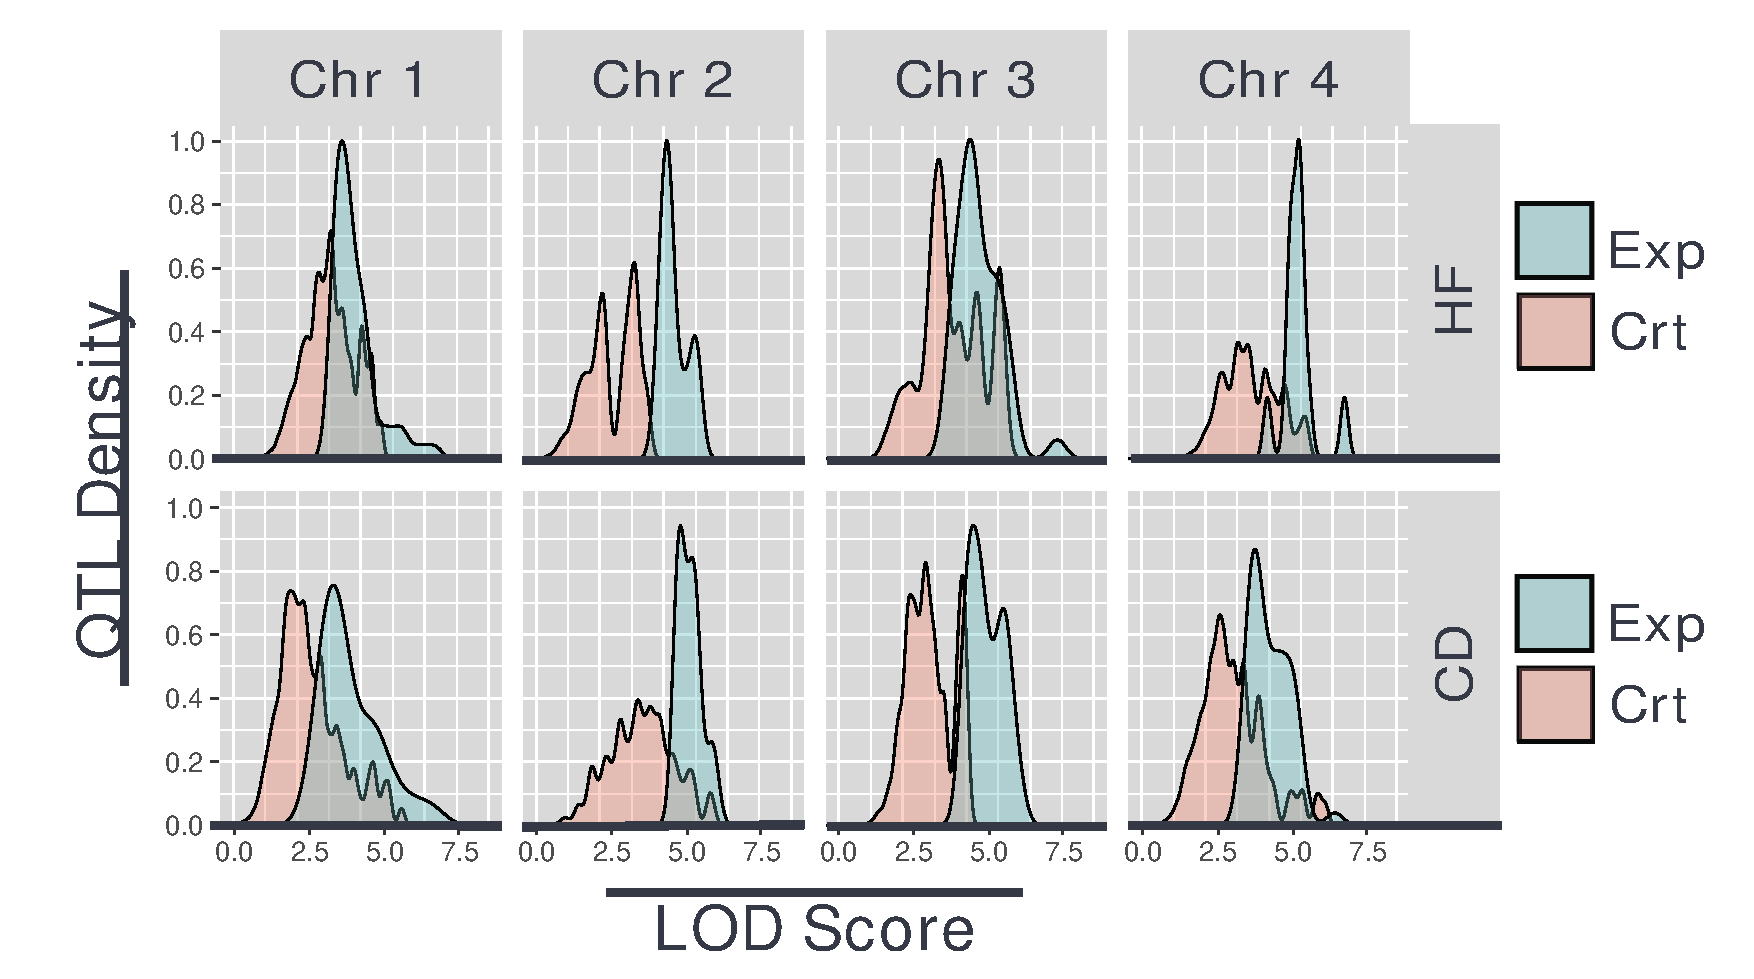
\includegraphics[width=1.2\linewidth]{QTL_Results/QTL_Densities.pdf}}
		\caption{This figure shows the raw computed LOD scores for the metabolites tested against the true genome array and the QTL LOD scores of testing those metabolites against a scrambled array of genotypes. The distribution of NUL LOD scores is given in red and the actual computed LOD scores are given in blue }
	\label{fig: Distributions of QTL LOD scores for all significant Age and Diet related Metabolites}	
\end{figure}
	
	From the assortment of metabolites found to have significant fold changes between the diet cohorts D-2-Hydroxyglutaric acid, pyruvate and glutathoine also have significant QTL results. The QTL for D-2 Isocitrate dehydrogenases (IDH) was already found in a previous study of a mouse cohort and servers as a validation that we have generated high quality data.  It is known that a mutant form of isocitrate dehydrogenase can also preform the reduction of D2-hyudroxglurate and it is seen as having a suggestive QTL. In the many genes that can be found in the QTL regions with the high LOD scores, D2HGDH is an already known catalyst for the production of the metabolite and allow the QTL to be solved quite readily.
	
    \begin{figure}
    	\makebox[\textwidth][c]{
		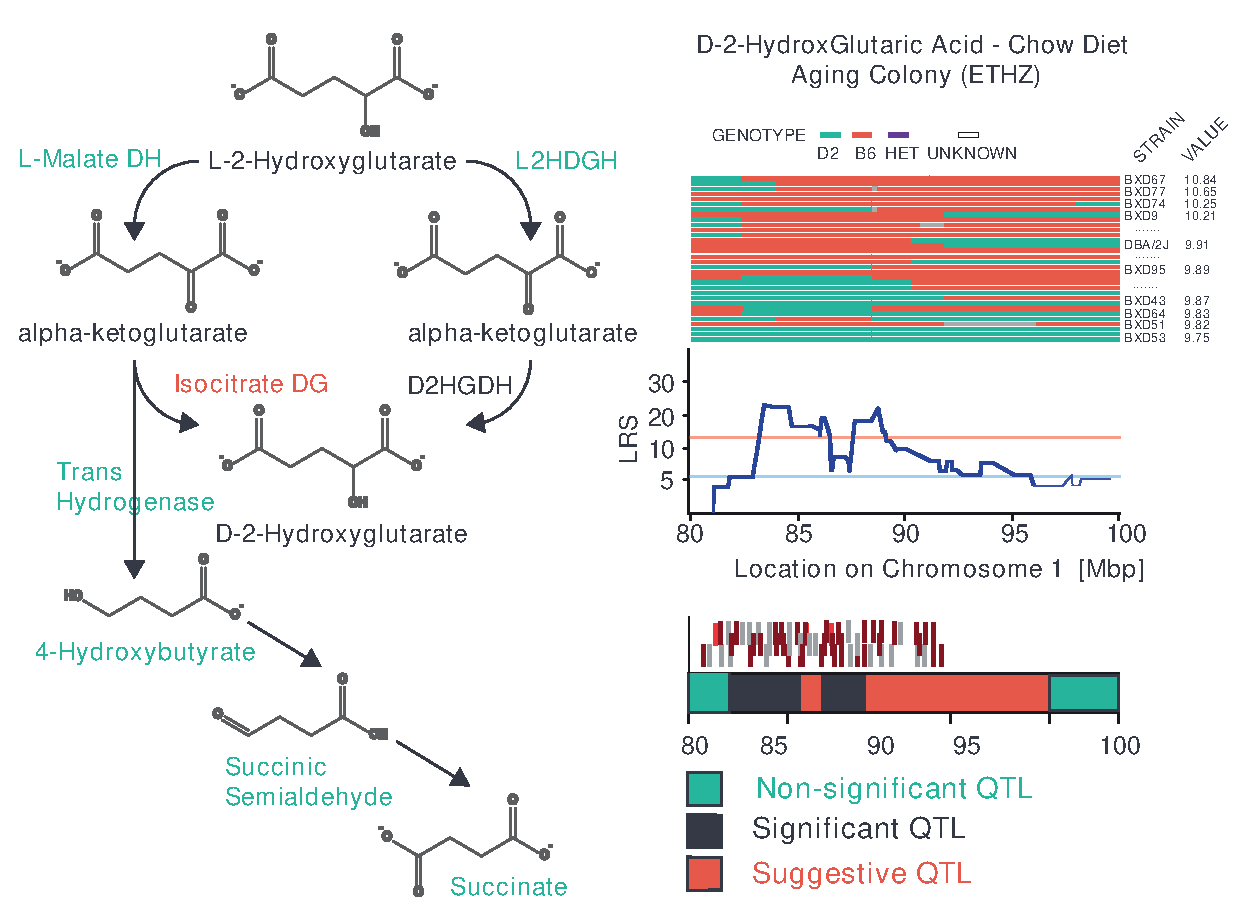
\includegraphics[width=1.2\linewidth]{QTL_Results/D2HG_QTL.pdf}}
		\caption{\textbf{Left:}Pathway showing the conversion of D-2-Hydroxyglutarate to $\alpha$-ketoglutarate through Dehydrogenases. Mutate forms for isocitrate DG and D2HGDH are known to perform this catalysis. Proteins that are contained in a significant QTL for D-2-Hydroxyglutarate are highlighted in black. Proteins in suggestive QTL are highlighted in red and non-significant loci are highlighted in green. \textbf{Right}The haplotype map at the loci on Chr 1 where the QTL is found is shown. On the right of the haplotype map, the values for D-2-hydroxylate are sort from highest to lowest. One can see that most of the strains with higher D2Hydroxyglutarate have the B6 allele and those that have the lower concentration of the metabolite have the D2 all. At the bottom of the panel, once see the areas of the chromosome where there are suggestive and strong QTLs and the lines above the schematic of the chromosome are the genes found in this reagion}
	\end{figure}
	
	\begin{figure}[ht!]
		\makebox[\textwidth][c]{
		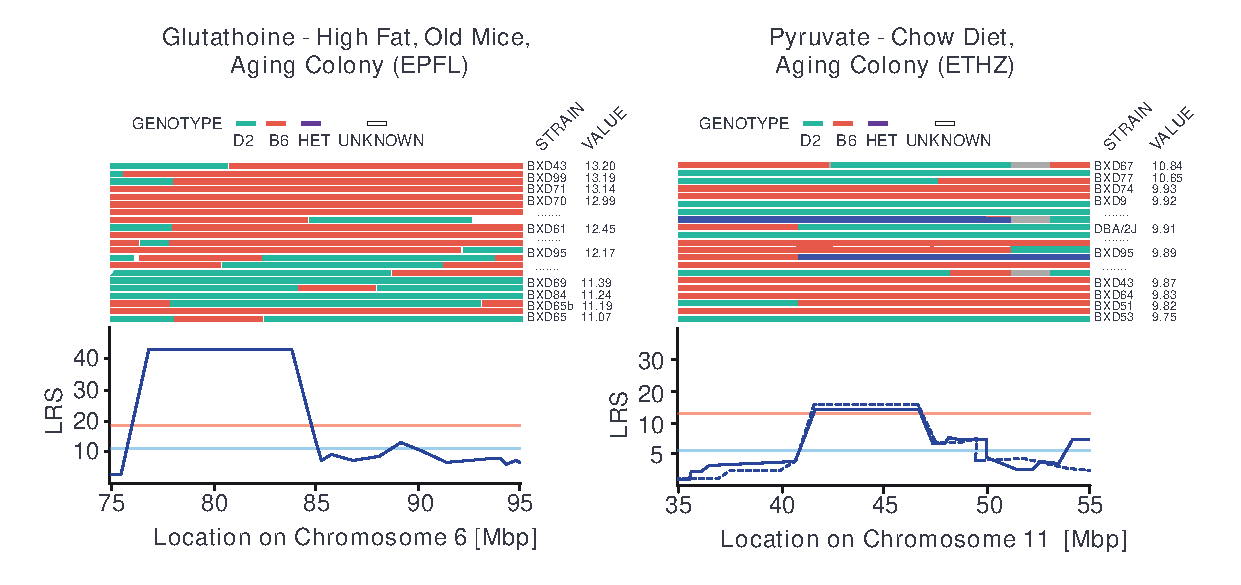
\includegraphics[width=1.2\linewidth]{3.Metabolomics/QTL_Results}}
		\caption{ The QTL haplotypes maps and QTL LOD scores for Glutahione and Pyruvate in the region the chromosome whre the higherst LOD score for the meatbolite is found}
		\label{fig:qtlresults}
	\end{figure}
	
    The QTLs for glutathione and pyruvate are not as obvious to solve as compared to D2GDH. If one looks at the strain wise values for pyruvate given on the right side the haplotype maps, there is a large jump between the two strains with the highest pyruvate levels and the rest. This is an indicator that this QTL may be outlier driven rather than driven by key genetic drivers for two separate population pools of low and high pyruvate mice. On visual inspection, the difference between the top two and the third mice is almost the same amount as the difference between the third highest mouse and the last. Even though each strain in this contains many biological replicates, there can still be chance fluctuations in the identified intensities of two or three mice in the same direction. Next, in inspecting the shape of the QTL between 40 and 47 mb on chromosome 11, it is evident that it is just barely significant. The dotted line is the QTL LOD score computed for mice that were both old \textbf{and} was on the high-fat diet in an attempt to see if there may be an interaction with HF fat diets in pyruvate only at old age. Lastly, when one looks int he QTL regions, it is strewn with ion transporters and Riken gene which would make the QTL difficult to solve. Pyruvate has such large number functionalities in cells and is involved in numerous metabolic pathways, which only confounds the problem \citep{Voet2011Biochemistry}.
	
    On the other hand, the peak for glutathione is robustly above the significance threshold. The values for glutathione within the strains range from 13.20 to 11.07 with a gradual transition between the strains that have the B6 locus in the 80 Mb region in chromosome 6 and those that have a D2 allele. Additionally, the chromosome is much sparser in this region that it is in the region for pyruvate. The function glutathione is also more focused hopefully making it easier to solve the QTL detected.

	
	\section{Metabolite Set Analysis}
	
    After the glutathione QTL was found, metabolize set enrichment analysis is used to determine whether there are changes in the metabolites that are upstream and downstream from glutathione to get more biologically meaningful results. Set enrichment analysis of any kind requires the use prior knowledge to determine the probability that pathways are significantly affected given a set its components. The classification is highly dependent on the quality the prescribed ontologies. Luckily there is extensive data on the disease-related network and physiological networks for \textit{Mus Musculus} within the metabolite analyst framework \citep{Xia2016UsingAnalysis}. In the figure given below the absolute correlation coefficients for metabolites from all mice in the study, metabolites from mice in a single diet and metabolites from a single diet and single pathways were computed. In the total metabolites space, there is a very slight correlation. Removing half the mice in the set that do not consume the metabolites in the CD, HF-specific metabolites shown in green show a slightly larger correlation coefficients. Lastly, when only metabolites, within a simple KEGG pathway, are queried for their correlation, it becomes quite evident that the respective concentrations metabolites within the functional pathway modules are actively transformed, generated from each other as they pass through the pathway. This is why on average the correlation coefficient for the in pathway metabolites is much higher. With this rationale, if we look at the full network glutathione.
	
	\begin{figure}[htb!]
	\makebox[\textwidth][c]{
		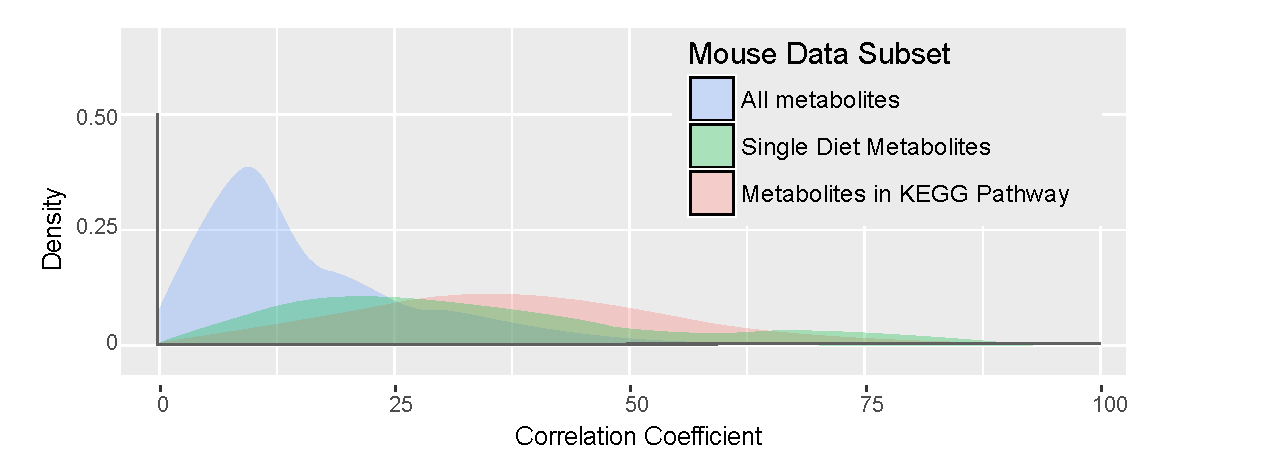
\includegraphics[width=1.3\linewidth]{3.Metabolomics/KEGG_Path_Correlations}}
		\caption{Correlation meatbolites In Metabolic Networks}
		\label{fig:keggpathcorrelations}
	\end{figure}
	
	Once the data for high enough coverage of a metabolic pathway is generated, it can be used for higher level interpretations in terms of pathways. This can be performed by putting the metabolite concentrations in the context of their catalyzing enzymes and gene pathways, visualizing all the fold changes on the pathway. The test is applied to determine whether a pathway is affected by either the age or diet segregation, is similar in nature to the question computing a QTL asks. In this case, we determine whether not the two populations of metabolites (HF/CD diet or Old/Young) projected on the pathway belong to the same population or not. If the mean fold change is conserved through many of the metabolites across two cohorts, they can be thought of as significantly effected\citep{Wishart2013}. Through this method, we see that the oxidized version of glutathione ( the red central node in figure \ref{fig:MSEA} ) is metabolized by rate-limiting enzymes and that it accumulates in older mice.  Thus this pathway is a hypothesis we can probe further one using Protein and RNA data.
	
	\begin{sidewaysfigure}
				\centering
		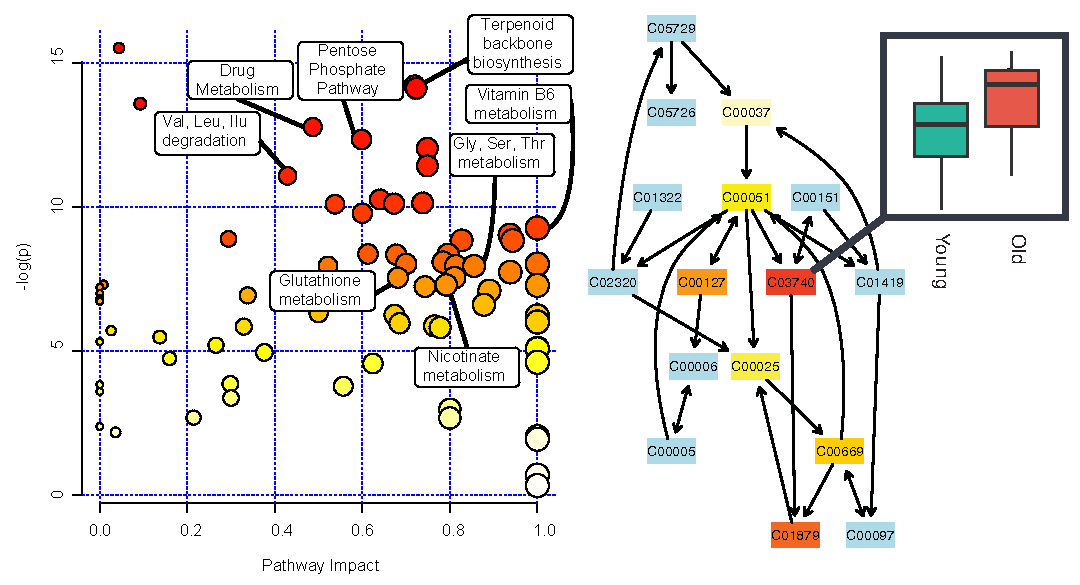
\includegraphics[width=0.99\linewidth]{3.Metabolomics/MSEA}
		\caption{\textbf{Left:}The results of the MSEA analysis show good coverage in many metabolic pathways, given in on the x-axis. On the y-axis is the probability the pathway is differentially affected between young and old mice. Pathways such as terpenoid backbone synthesis, glycine, serine and threonine metabolism and vitamin b6 metabolism are both well covered and have significant fold change differences between the young and old mice. Two pathway of particular interest to the Auwerx lab, glutathione metabolism, and nicotinate metabolism are also significantly effects but have lower coverages, making flux estimations in the pathway difficult. \\ \textbf{Right:} Glutathione metabolism is shown. The synthesis of GSH from glutamate, cysteine, and glycine is catalyzed sequentially by γ-glutamylcysteine synthetase (GCS) and GSH synthetase. This pathway occurs in virtually all cell types, with the liver being the major producer and exporter of GSH. Glutathiones scavenges ROS and radical species and oxidized to glutathione disulfide(GSSG). It can be reduced to GSH by the NADPH-dependent glutathione reductase which may be less effective in older mice leading to the build-up of oxidized glutathione shown in the box plot. \citep{Wu2004Glutathione}}. 
		\label{fig:MSEA}
	\end{sidewaysfigure}
	
	
	\chapter{Proteomics}
	
	\section{Introduction to MS Proteomics}
    Proteins are involved in almost all the functional components of a cell, participating in enzymatic, structural and signaling modules that determine the phenotype \citep{Hartwell1999FromBiology}. Historically, quantitative protein studies have been performed on a small subset protein for which high-quality validated anti-bodies exist. Unfortunately, anti-bodies experiments show a great deal cross-reactivity, are time-consuming to perform and are poorly multiplexed\citep{Solier2014Antibody-basedLimitations}. Even though ELISA and western blots can show a much higher sensitivity than MS techniques and can be performed on a large scale using robotics, these assays suffer some poor resolution of relative protein concentrations and specificity as compared to mass-spectrometry methods \citep{Solier2014Antibody-basedLimitations}. As a result, mass-spectrometry techniques have become the tools choice for proteomics studies. With more sophisticated data analysis techniques and faster, higher resolution instruments available on the market, simultaneous and comprehensive coverage protein concentrations from all functional classes in the proteome can be done, allowing the holistic assessment the overall biochemical state a sample \citep{Schubert2017QuantitativeResearch}.
	
    The earliest use mass spectrometers with proteins were in top-down sequencing application. In MS-sequencing, a protein is incompetently digested, then single amino-acid residues are removed from the c-terminus and analyzed by a mass spectrometer to elucidate the sequence of the fragment. Once, the sequences of many small fragments are uncovered, overlapping peptide sequences are used to sequentially elucidate the amino acid sequence of the whole peptide\citep{Steen2004TheSequencing}. Bottom-up or peptide-centric methods are used to analyze protease digestions and prototypic peptides to perform quantification on a variety proteins in a mixture. Contemporary applications MS-Proteomics include DIA(data independent methods) which uses spectral libraries to accurately quantify large number proteins in a sample SRM(selective Reaction Monitoring) in which a pre-selected group proteins can be monitored at high sensitivity\citep{Picotti2012SelectedDirections} and DDA(Data Dependent Acquisition) methods which can be used for deep proteome mapping \citep{Nagaraj2011DeepLine.} and proteome-wide quantifications of model organisms \citep{deGodoy2008ComprehensiveYeast}. In all three methods, fast, high-resolution mass spectrometers that have the ability to analyze specific bands the mass range are required to obtain detailed information on what ions arise from fragmenting selected parent ions.
	
	
	\begin{figure}
		\centering
		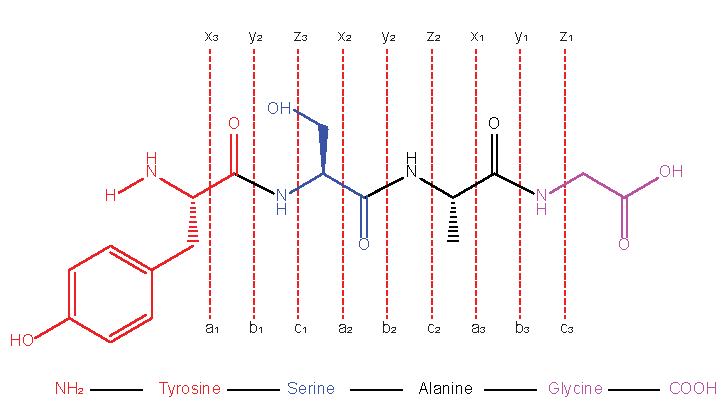
\includegraphics[width=0.6\linewidth]{3.Proteomics/peptide_frags.pdf}
        \caption{The proteomics nomenclature first purposed ion 1985 by \citep{Roepstorff1984LetterEditors} used to describe sequence fragments is maintained as a convenient method for referencing fragment by the site they are cleaved from the peptide. Starting from the N-terminus, the ion is the fragment generated by a cleavage before the carbonyl, the b fragment is a cleavage after the carbonyl-forming the acylium ion and the c ion is a fragment derived from a cleavage after the amide bond forming an ammonium ion fragment. The converse is true for z, y and x ions which denote the same fragments starting instead from the carboxylic acids terminus. The subscripts denote the residue number from the N or C terminus the cleavages occurs \citep{Roepstorff1984LetterEditors}.}
		\label{Tri_peptide_seq}
	\end{figure}
	
	
	\subsubsection{Proteome Data acquisition Paradigms}
	
    With Data Dependant acquisition a full spectrum the peptides that elute off a column into the mass spectrometer are analyzed. The instrument alternates between scanning the total ions recorded at the MS1 level (full scan mode) and precursor mode in which ions that have high intensities in the full scan are analyzed after being isolated and fragmented into smaller fragmentines\citep{Bateman2014MaximizingDDA.}. It is an unbiased method for observing as many peptides at the MS2 level as possible within a single duty cycle. Although DDA methods allow for detection significant portions mammalian proteomes it does not provide robust quantification all detected peptides\citep{Richards2015ProteomeDeep.}.
	
	\begin{figure}[ht]
		\centering
		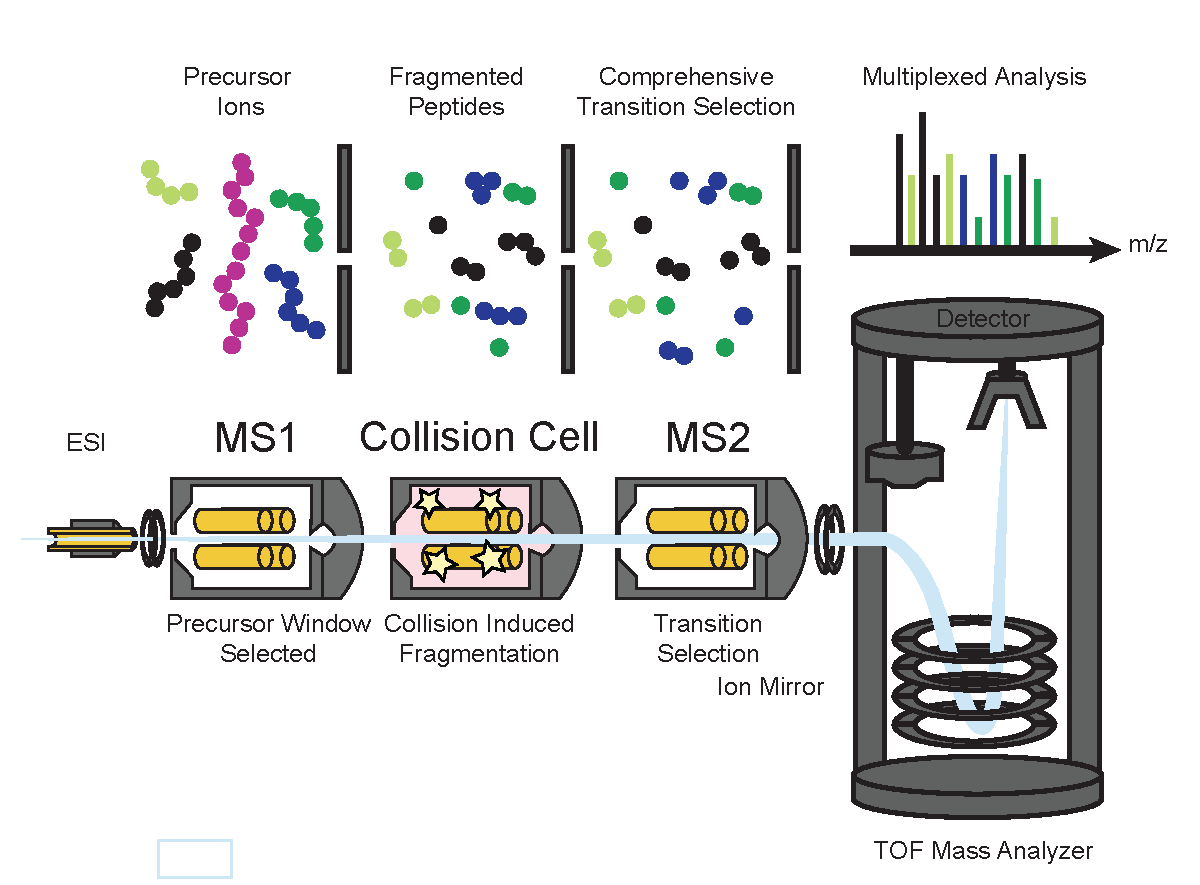
\includegraphics[width=0.9\linewidth]{3.Proteomics/Mass_Spec.pdf}
		\caption{Schematic AbSCiex 5600+ Triple TOF Mass Spectrometer used for DIA/SWATH Experiments. One can see the electro-spray injection(ESI)  needle on the left followed by three quadrapoles and a Time of Flight(TOF) Mass Analyzer. Digested peptides are separated using a high pressure LC column and then injected into the mass spec through the ESI needle. In DIA mode operation, the first quadropole (\textbf{MS1}) acts as a bandpass filter allowing a selected range peptides through to the collision cell. Ion transmission through a quadrapole can be tuned by applying combinations DC and RF voltages that are resonant with a certain interval m/z ions. In this case the \textbf{purple peptide} is too large and is filtered out. The transmissive ions are known as the \textbf{precursor ions} are fragmented through collision with neutral gases such as \ch{N2} or \ch{Xe} in the collision cell. The collective fragments from all the precursors are known as \textbf{fragmentines} or \textbf{transitions} are focused into the time-\cite-flight chamber for mass analysis. The resulting spectra (shown above the TOF analyzer) is a composite all the fragmentines from the precursor ions}
		\label{Schematic MS-TOF in DIA mode operation}
	\end{figure}
	
	
    Data independent acquisition methods such as SWATH\citep{Gillet2012TargetedAnalysis} acquire a signal from a large band MS1 peptides and to do not use the MS1 peptide intensities to determine which peptides precursors are selected for further fragmentation\citep{Venable2004AutomatedSpectra}. This is in contrast to Data Dependant mass spectrometric techniques in which fragments with the highest intensities in the MS1 space are selected by the machine to be fragmented and further analyzed in the MS2 space. Signal intensities in the MS1 space can be highly stochastic meaning peptides may not always be selected by the mass spectrometer in DDA mode between samples if they do not consistently show the same high-intensity peaks. Another key difference between DIA and DDA methods is that while DDA machines run on an alternative fulls scan and precursors duty cycles, a SWATH machine runs on fixed pre-programmed duty cycles, where swath acquisition windows are programmed to scan over a large mass range in increments 5m/z to 25m/z\citep{Rost2017AutomatedChromatograms}. As the wide precursor isolation window moves over a mass range between [400-1000] in 5-25m/z intervals, all the peptides in the interval are fragmented and analyzed together. Complex MS2 spectra are generated when all of the fragmentines of the precursor isolated space are recorded together and necessitate the use of computational tools to deconvolute. 
	
    The most common instrumentation used in SWATH is the quadrupole time-flight mass spectrometers, A schematic an AbSciex triple TOF is shown in figure \ref{Schematic MS-TOF in DIA mode operation}. Irrespective the instrument being used, accurate SWATH implementation have a quadrupole which can act as a selective band filter for precursor selection and a high-resolution mass analyzer than produce high-quality MS2 spectra.
		
	\begin{figure}[!htb]
		\makebox[\textwidth][c]{
		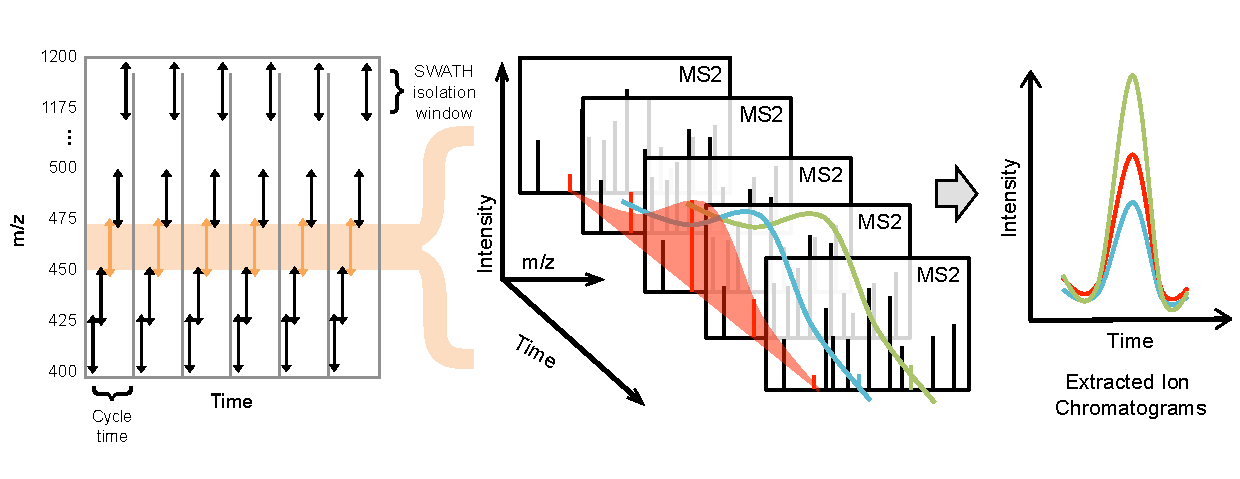
\includegraphics[width=1.2\linewidth]{3.Proteomics/XIC.pdf}}
		\caption{ Figure adapted from \citep{Rost2017AutomatedChromatograms} Illustration the SWATH-MS Duty cycle. (1) As peptides elute of an orthogonal chromatography column into the mass spectrometer, a window mass ranges OR SWATHS are isolated and fragmented. (2) The ions that results from the fragmented peptides is recorded as a convoluted spectrum including fragments from the three \textbf{Red, Green and Blue} peptides. For each the swatch, there is a 100 ms acquisition cycle in the MS2. From 400-1200 m/z this makes a full duty cycle 3.2 seconds. (3) Once the acquisition is complete, specific ion fragments can be extracted from the multiplexed peptide spectra to produce ion chromatograms for peak groups. }
		\label{fig:Principles SWATH MS}
	\end{figure}
	
	In the figure \ref{fig:Principles SWATH MS} the red and blue peptides can be use to illustrate the principles of  SWATH sampling of the precursor space. Each consecutive window moving in the z-axis out the page shows an MS2 spectra at subsequent time points of the chromatographic separation. The red and blue digested protein (we can assume they a have m/z 500 and 502 respectively) elute off a chromatography column and are injected into the first mass analyzing quadrapole. An the MS1 a precursor isolation space 5m/z is used and selects both the red and blue peptides for fragmentation in the collision cell. Both peptides are co-isolated, co-fragmented and co-analyzed leading to the MS2 seen in the windows of figure \ref{fig:Principles SWATH MS}. As a result, fragmentines from all the precursors are present in the final multiplexed data. By determining all the fragmentines that are known for a single peptides, the multiplexed MS2 recordings of the transition mixtures can be deconvoluted. 	In this way, the continuous monitoring of the peptides is done both in terms time and MS2 signal thus comes at the cost added complexity in separating and quantifying the signal from different precursor peptides. However, When the instrument is forced to fragment all the precursors in every duty cycle within the limit detection, the result is a consistent quantification all precursors in the sample \citep{Gillet2012TargetedAnalysis}. 
	
	\subsubsection{DIA SWATH Operation}
	\begin{figure}[t!]
		\centering
		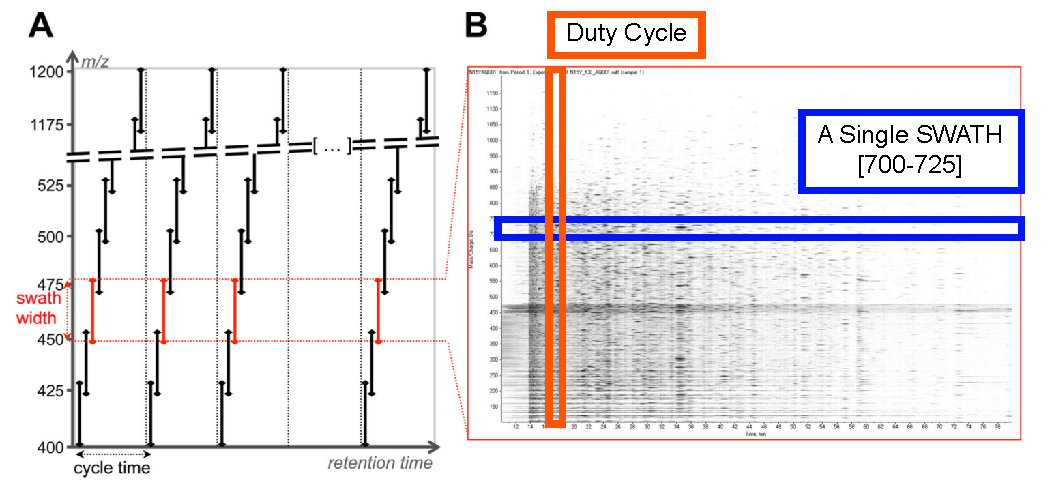
\includegraphics[width=1.0\linewidth]{3.Proteomics/DIA_SWATH_Principle_1.pdf}
		\caption{Figure adapted from \citep{Rost2014OpenSWATHData} A.SWATH duty cycle schedule. B. Final 2D chromatogram LC-MS SWATH Data C.Reconstructed and aligned XIC D.  A. The x-axis represents the chromatographic dimension and the y-axis the m/z domain with the vertical arrows shows the m/z acquisition windows. The signal intensities the peptides at each mass/charge unit at a given point in the elution shown in the grey and black scale. Each one the black dots seen is  a different precursor ion.}
		\label{Deconvoluted MS2 Spectra}
	\end{figure}
	
    In figure \ref{Deconvoluted MS2 Spectra}, an example the data acquired from the initial implementation SWATH Acquisition can be seen. A SWATH (highlighted in blue in panel B) is the collection fragments that are acquired in a single mass isolation window, in this case, 700-725 throughout the chromatographic separation. The cycle time is highlighted in red. The quantitative accuracy the proteomic analysis is inverse dependent between the SWATH-window and dwell time on each window \citep{rost2017automated}. As SWATH-MS has a chromatographic separation, the cycle time must be sufficiently small to resolve multiple close peaks in a single SWATH.On a 400-1200 m/z range with 25m/z swaths, a machine with 100 ms dwell time on every acquisition window require 3.2 seconds per cycle. Increasing the cycle time increases the accuracy the fragmentines being quantify but reduces the resolution the chromatographic peak each peptide's elution\citep{Lange2008SelectedTutorial.}. Additionally, the precursor isolation window can be tuned to use smaller 5m/z wide swath windows in the lower m/z peptides [400, 600] where there is a large number eluting peptides and larger windows in the [1000,1200] regime where the number of quantified peptides is much smaller. This can increase the number peptides detected by 10-15\% in complex samples where multiple peptides are co-isolated in a single swatch-window.
	
	\subsection{Extracting Peptide Chromatograms}
	
	In contrast to DDA acquisition, in which all the MS2 spectra come single peptides fragments, the MS2 spectra produced with SWATH contains peaks from many precursors and are not directly searchable against a peptide database. Processing the spectra is done using a C++ distribution called OpenSWATH which allows the automated processing the SWATH data and spectral library\citep{Rost2014OpenSWATHData}. In figure \ref{fig: Complex Spectra XIC} the top panel shows MS2 spectra of a swath from 700-725 which includes fragments from the peptide \textbf{WIQDADALFGER}. The lower panel shows DDA spectra, our prior knowledge, two fragments \textbf{WIQDADALFGER} that were isolated by the mass spec and quantified in DDA mode. In figure\ref{fig: Complex Spectra XIC}D. the spectral features from two fragments y4 and y10 identified both DIA(top) and DDA experiments(bottom) are highlighted. 
	
    In a DDA experiment, the y4 and y10 fragments would have high intensity and would be selected by the machine to be isolated for fragmentation thus allowing us to determine the major characteristic peaks from these precursor ions. The pattern of peaks detected at the MS2 is a unique fingerprint signature for each precursor fragment\citep{Gillet2012TargetedAnalysis}. This fingerprint can be used to assign fragmentine peaks to a specific fragment and peptide in a convoluted DIA MS2 spectra. Once the major fragmentines from the precursor peptides can be identified in the complex spectra using previously determined DDA signatures we can plot fragmentine intensities against the chromatographic time dimension and signal group overlapping peaks begins to appear, as seen in fig \ref{fig: Complex Spectra XIC}.C. If many fragments are derived from a single precursor ion, the peaks result in overlapping extracted ion chromatograms(XICs). Statistical analysis can then be used to score peaks taking into account the peak shape in elution profile. Lastly, the maximum intensity of the highest peak for each the fragments is used for peptide quantification. 
	
	\subsection{SWATH MS for BXD Mouse Liver Proteomics}
	
    To analyze complex proteins mixtures extracted from the BXD Mouse livers, SWATH is ideal as it allows the quantification of a large set proteins across multiple samples and providing a consistent number protein quantified, with high accuracy, reproducibility and sensitivity. Using DDA methods, many more proteins can be detected but the measurement is not reliable across many samples. SRM, a classical targeted proteomics has slightly higher sensitivity compared to SWATH but the number protein that can be quantified is relatively discrete. With certain optimizations SWATH shows coverage comparable to MS1 label-free quantification as in shotgun identification and sensitivity comparable to the performance of SRM \citep{Liu2013QuantitativeSWATH-MS}. In a side-by-side comparison, plasma protein detection by SRM and SWATH \citep{Liu2013QuantitativeSWATH-MS} show similar CVs and slightly lower quantification proteins (33 vs 37) in SWATH. 
	
    Another distinct advantage of using SWATH proteomics is the ability to re-process data post hoc. If an XIC) hows two probable elution peaks for a precursor, it may be difficult to determine which chromatographic peak should be used for quantification. In SWATH, all transitions data is saved, meaning different transitions can be added to the composite XIC to determine which is the correctly eluting peak \citep{Gillet2012TargetedAnalysis}. Moreover, if a major peak in the XIC is distorted due to some interfere, one could simply select a different peak to use for quantification. Unless a sufficient variety of peaks were sampled in SRM this would not be possible post-hoc\citep{Gillet2012TargetedAnalysis}. Lastly, SWATH allows for iterative mining proteomic data enabling the biologist to simply reprocess the data and select peaks for different proteins of interest rather than having to re-perform the experiment targeting a different set of proteins in the same sample \citep{Gillet2012TargetedAnalysis}.	
	
	
	\subsection{DDA Spectral Library Generation}
	
	\begin{figure}[ht]
		\centering
		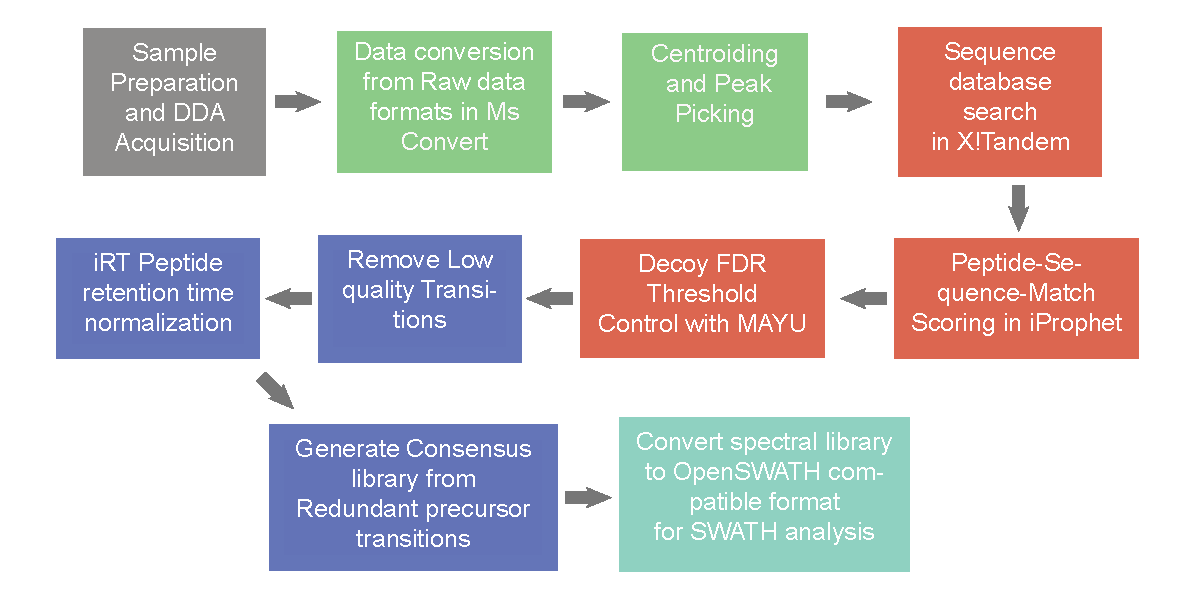
\includegraphics[width=\linewidth]{3.Proteomics/Spectral_Library_Gen.pdf}
		\label{Spectral Library Generation Road Map}
	\end{figure}
	
    \textbf{Raw Data Processing and Conversion:}\\
	For spectral library generation, representative samples from the full cohort of samples need to analyzed in DDA mode in order to tabulate pertinent information about the peptides and their transitions. High-quality protein libraries from a 58 mouse liver samples run in shotgun mode have already been constructed in previous BXD mouse liver studies which allow us to use the previous data \citep{Williams2016SystemsFunction}. The data from these runs have to be centroided and converted from a proprietary to an open source format such as mzML or mzXML in order to perform the subsequent processing steps. A range converters can be used however, the centroiding algorithms may change the appearance XICs depending on whether the maximum peak height or peak integral is used. ProteoWizard-MSCovert which is specifically written for processing LCMS data using the max peak height and generates the optimal centroid data for database searching \citep{Kessner2008ProteoWizard:Development}. 
	
    \textbf{Peptide Sequence Annotation:}\\
	The next steps, database searching, scoring and spectral library generation can all be performed with using components an open-source suite protein data processing packages known as TPP (Trans Proteome Pipeline). Using, iProphet \citep{Shteynberg2011IProphet:Estimates.} all the MS2 spectra are searched against multiple sequence database search engines such as X!Tandem and Comet\citep{Eng2013Comettool} which can annotate spectra by comparing experiential peaks to expected peaks from in-silico digested libraries within given mass defect tolerances. Rather than exhaustively searching all peptide-sequence combinations iProphet assigns a match with the highest probability and quality score to each peptide-spectrum match(PSM) through a penalized greedy search algorithm \citep{Shteynberg2011IProphet:Estimates.}. 

	If an MS2 spectrum is erroneously annotated, the error will propagate to the DIA analysis and peaks found in the DIA quantification will be thought to have originated from the wrong peptides. MAYU is used to need to perform a false discovery rate estimation at the PSM, peptide and protein levels \citep{Reiter2009ProteinSpectrometry}. It takes the iProphet output and generates robust empirical FDR estimate using the target-decoy technique\citep{Elias2007Target-decoySpectrometry}. A 1\% Protein FDR, 0.2\% Peptide FD, 0.08\% PSM FDR and iProphet score threshold 0.9774 is used to keep only high-quality spectra in the library. 

	\textbf{Elution Time Normalization:}\\
	In order to use a DDA spectral library to interpret DIA data, the peptides in the DDA library must elute at a similar time interval to the DIA quantifications. This is an issue because the absolute retention different peptides may vary on the order minutes between runs, columns and mass spectrometers. In order to normalize the elution behavior between runs, 11 intensity and retention time standards (iRT) peptides are spiked into all sample at a high concentration \citep{Bruderer2016HighprecisioniRT}. These peptides elute at regular intervals on the LC gradient. The elution time of the second peptide is set at an arbitrary unit of 0 and the 11th at 100. A linear fit between the interim peptides allows us to project all sample peptide retention times onto the 0-100 scale instead of the chromatography time scale. The same iRT peptides are also spiked into the DIA samples allowing us to predict when the samples peptide will elute reducing the search space for where a peak corresponding to a peptide in the DDA library and DIA data \citep{Bruderer2016HighprecisioniRT}.

	\textbf{Spectral Library Consolidation:}\\
	In a given DDA experiment, there is a significant amount redundancy in MS2 data recorded for each MS1 precursor ion. MS2 fragmentation can be triggered multiple times or triggered stochastically as mentioned before, resulting in redundant MS2 spectra in our data. Using SpectraST a consensus spectra consolidating the features of all MS2 spectra for a given MS1 peaks can be generated. This is done by averaging the intensities of replicate peaks and removing individual MS2 spectra that do not conform to the mean spectral patterns\citep{Lam2008BuildingProteomics}. In the end, 5/6 transitions in multiple charge states are taken for every precursor ion \citep{Schubert2015BuildingData}. Transitions that are found in the MS1 data or have an m/z below 400 are noisy and thus excluded from the library. Once a library of MS2 spectra with sufficiently high PSM score, low FDR rate, and minimal redundancy is produced, it can be converted into the TraML for integration into the OpenSWATH package for analyzing DIA data.
	
	\begin{figure}[ht]
		\centering
		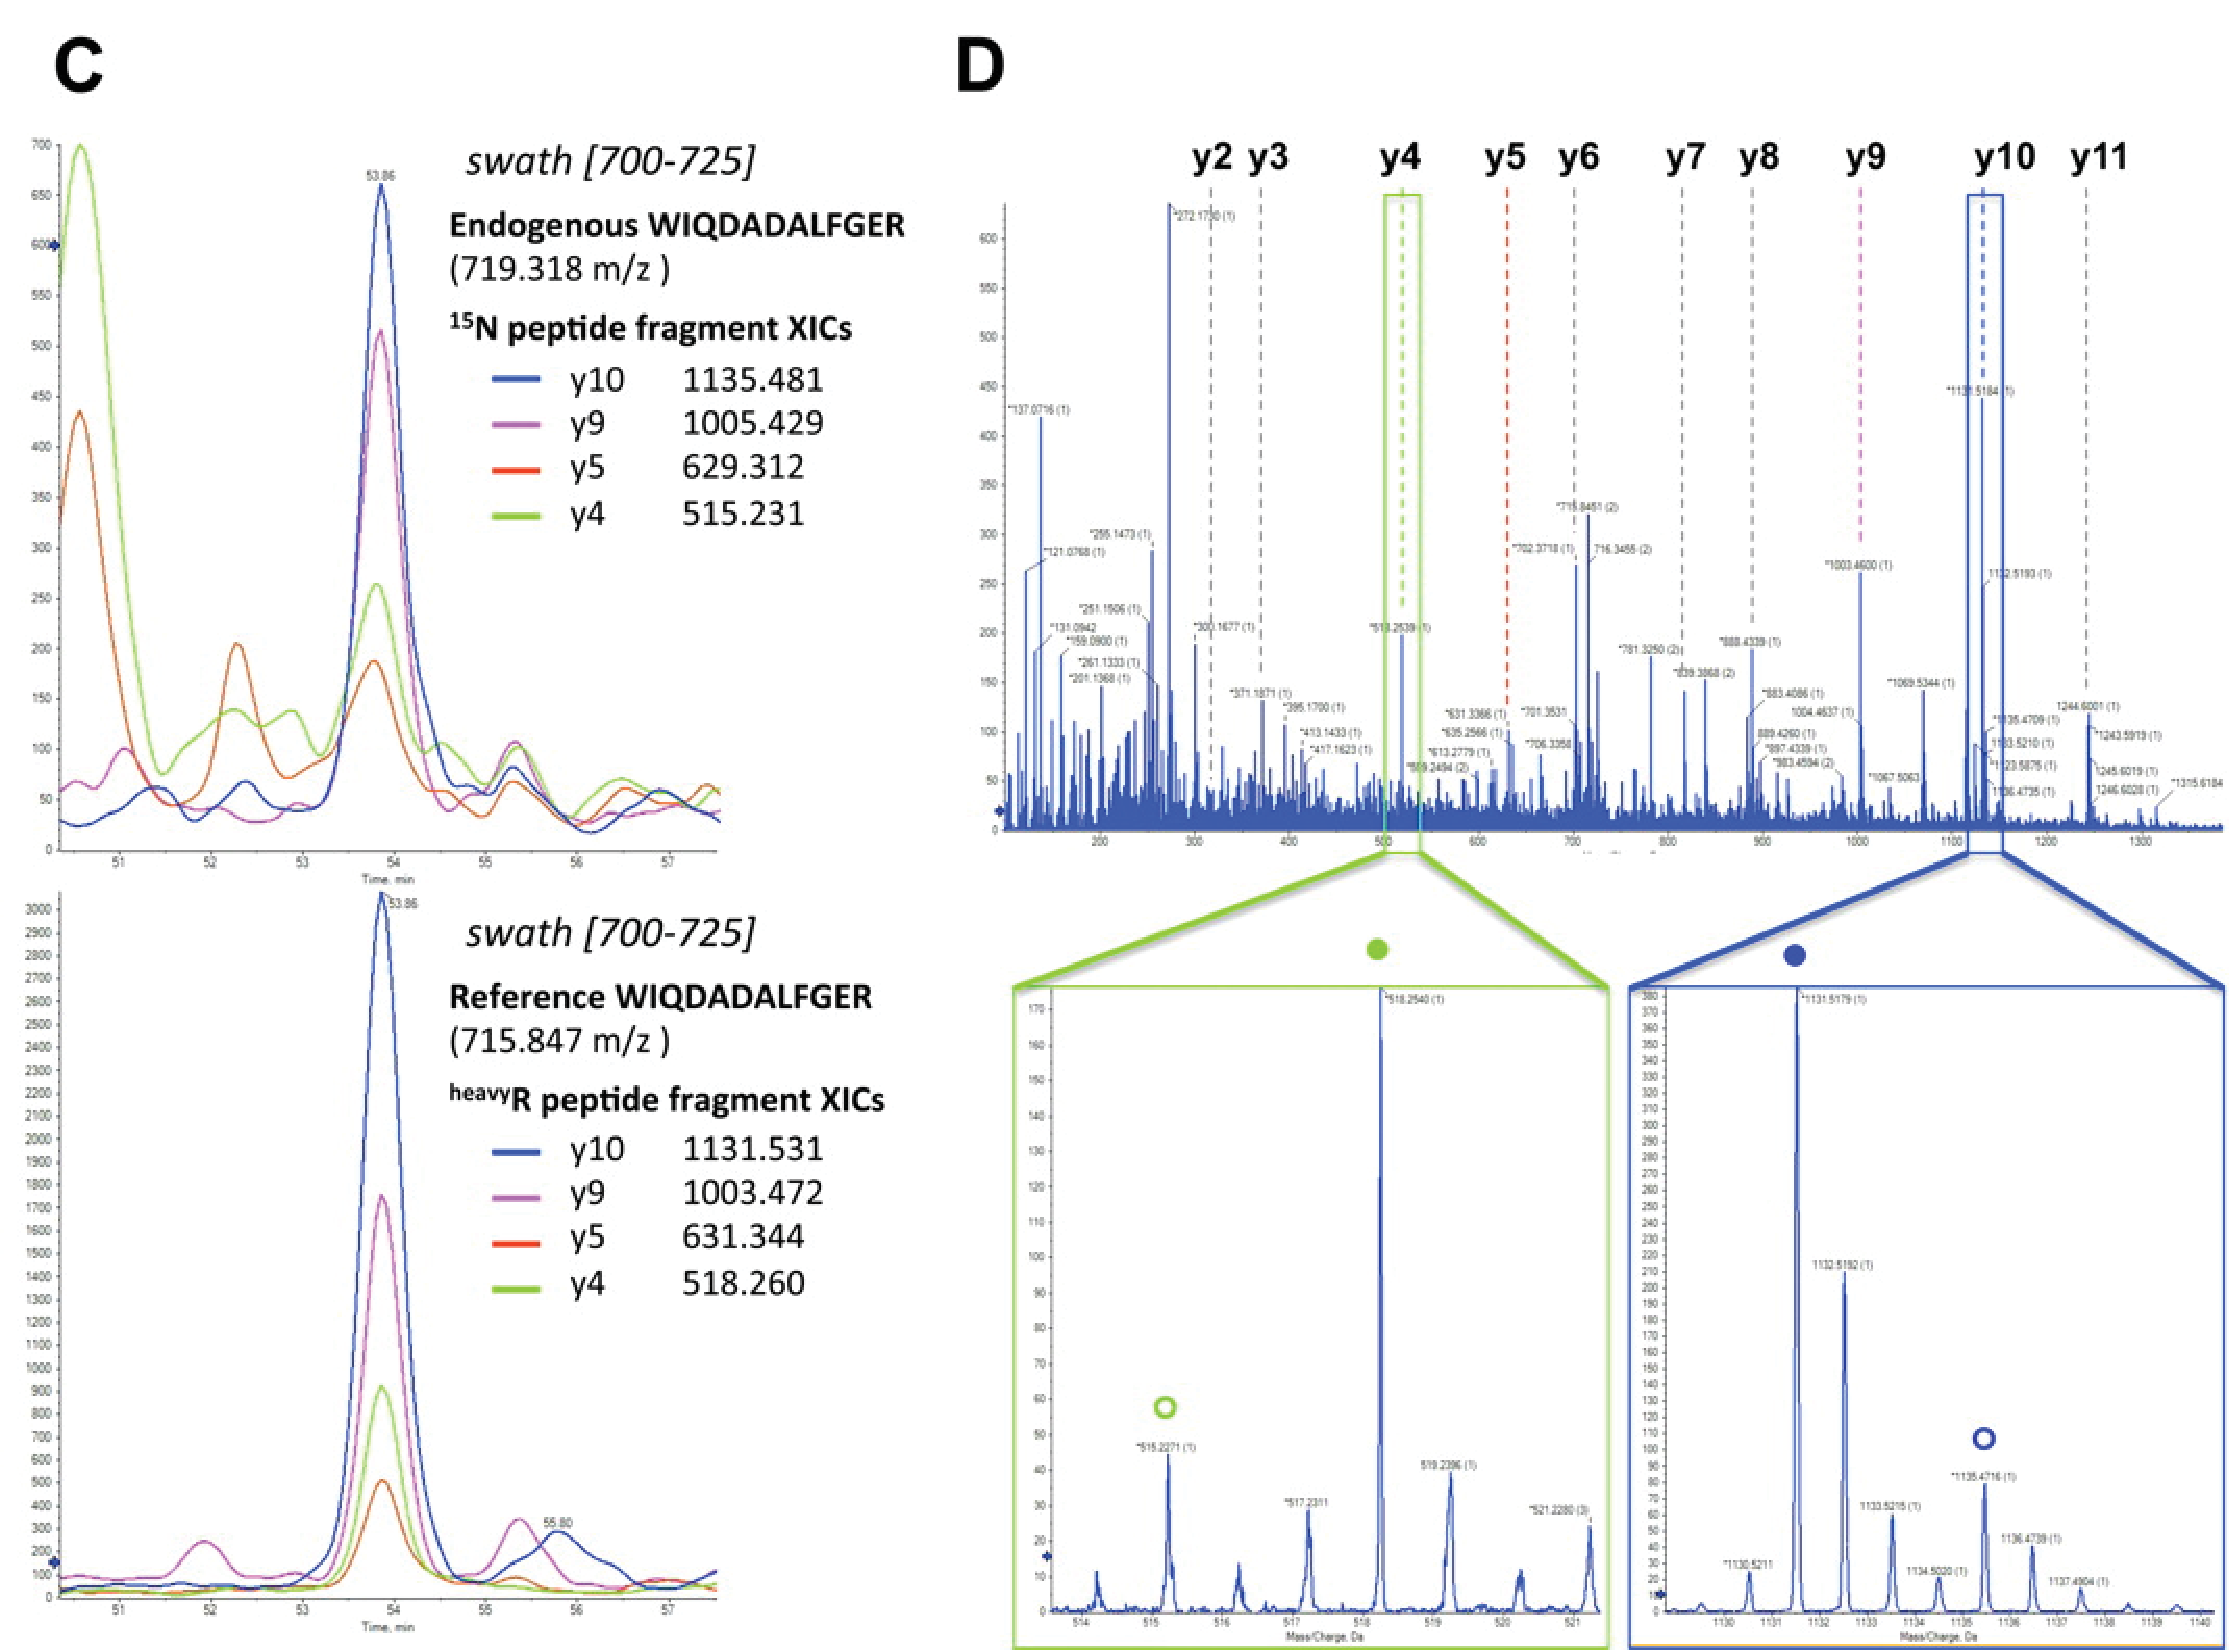
\includegraphics[width=1\linewidth]{3.Proteomics/DIA_SWATH_Principle_2.pdf}
		\caption{Figure adapted from \citep{Gillet2012TargetedAnalysis} \textbf{Top:} Right: DIA M2 spectra of the 700-725 m/z swatch for the peptide WIQDADALFGER Left:The extracted ion chromatogram for the peptides determined using the y10, y8, y4 and y5 overlapping peaks around the 54min elution time\\ \textbf{Bottom:} Right: M2 spectra from the y4 and y10 peaks showing all of the fragmentines from the two fragments break down into when the peptides are isolated and subjected to collision induced dissociation Left: The XIC from for the peptide WIQDADALFGER after scoring and aligning the various MS2 peaks to determine the most likely peak}
		\label{fig: Complex Spectra XIC}
	\end{figure}
	
 
    \subsection{Experimental Proteomics Protocol}

	In order to samples with SWATH-MS and DDA, proteins must be extracted from the liver tissue and digested into shorter peptides. Trypsin is used to cleave proteins at long basic amino acids after which the samples are cleaned to remove salts, lipids and other metabolites that can interfere with the LC-MS chromatography column. As the DC bias can change on the mass spectrometers detector, many internal standards as prepared in order to normalize the peak times and peptides intensities. For 20–300 \si{\micro\gram} protein extracted from the BXD livers, 20 pmol/\si{\micro\litre} fetuin B and 20 pmol/\si{\micro\litre} alpha1-acid glycoprotein (AAG) in addition to a set universal protein standards (UPS1) are spiked in on the day analysis. 

	On average, 100\si{\micro\gram} of protein is extracted from each sample. For the initial extraction from the liver tissue, the sample cuvettes are filled with acetone which disrupts the cells membranes and precipitates the proteins. Next, urea and bicarbonate buffer are added to denature the peptides and facilitate digestion by trypsin. Iodoacetamide and dithiothreitol are di-sulfide reducing agents added to the mixture to prevent cross-linking between the extracted protein \citep{Voet2011Biochemistry}. The protein samples are incubated in the denaturing mix for an hour before trypsin is added to digest them overnight. The digestions should not be longer than 24 hours, as trypsin can hydrolyze bonds within its own backbone creating large peaks in the mass spectra. Next, peptides are cleaned using a $C_18$ column. The samples are washed with \ch{MeOH} followed by mixtures \ch{ACN:H2o} with increasing proportions water to remove polar impurities. Using a 1:1 mixture \ch{ACN:H2o}, the peptides can be eluted. The LC solvent gradient goes from a 2\% \ch{ACN} solution to a 50\% solution. The column therefore also removes any peptides that could not be resolved with this solvent gradient. Lastly, the digested peptides are centrifuged and dried for storage at $80^\circ$C. 

	On the day of the mass spectrometry runs, the dried samples are resuspended in a mixture of\ch{ACN:H2O} 2:98 + 0.1\% FA to a target concentration around 250–1000 ng\si{\micro\litre}. The samples are adequately agitated and sonicated to free proteins that may be stuck to the walls of the cuvette. A final centrifugation removes residual impurities that may cause issues with the mass spectrometer. The UPS1 peptides are spiked into the samples and act as a control for the sample injection. Indexed retention time (iRT) peptides which elute in a well-defined interval on LC are added to control for variation in the chromatography between samples \citep{Escher2012UsingPeptides.}. Once the samples and internal injection, time and digestion control are loaded into MS tubes. The samples are ready for injection into the mass spectrometer in either DDA mode for library generation and DIA/SWATH mode for quantification.
	
	\section{Data Analysis}

	Once the mouse liver proteomics samples have been digestion, analyzed in the mass spectrometer and processed using OpenSWATH an excel sheet with all the transition intensities, peptide and protein can be exported. Once the data is in this tabular form, the remainder of the analysis is done in R.
	
	\begin{figure}[htb!]
		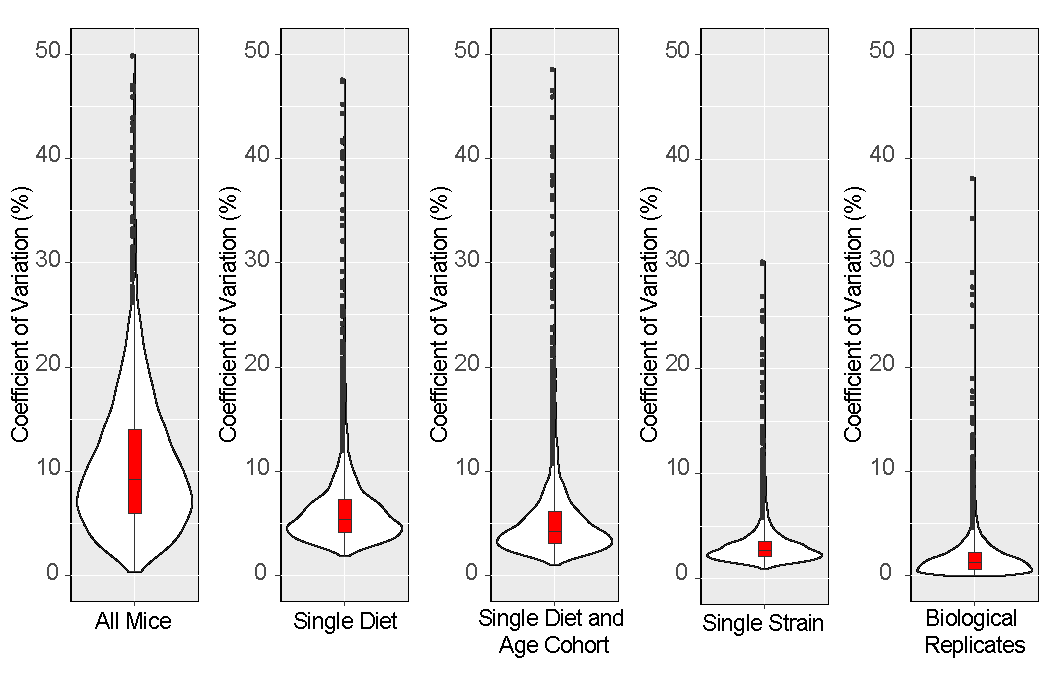
\includegraphics[width=\linewidth]{3.Proteomics/protein_cvs_figure.pdf}
		\caption{Coefficient Variation SWATH-MS Run between Mice measured in two batches}
		\label{CV Analysis Proteomic Data}
	\end{figure}
	
	\section{Quality Control}
     
    The protein level intensities are computed by taking the mean intensity the three most intense peptide fragment peaks. As a preliminary quality check, the coefficient variation is computed for the protein level (\ref{CV Analysis Proteomic Data} ). Across all the mice, there is an 8\% coefficient variation. In contrasts to metabolomics where 8\% coefficient variation can be seen in the injection replicates, peptides are more homogeneous in their physiochemical properties and are able to be prepared and analyzed in a more reproducible manner. Additionally, there are many more layers post-processing SWATH data in comparison to shotgun-MS data. The CV for proteins in mice that eat single diet is 5\%. Once the age is controlled for, this dropped even lower to 4\%. Between biological replicates, the variation is minutely allowing for the detection small changes between cohorts.
    
     \subsection{Batch Effects}   
     
     \begin{figure}[ht!b]
     	\centering
     	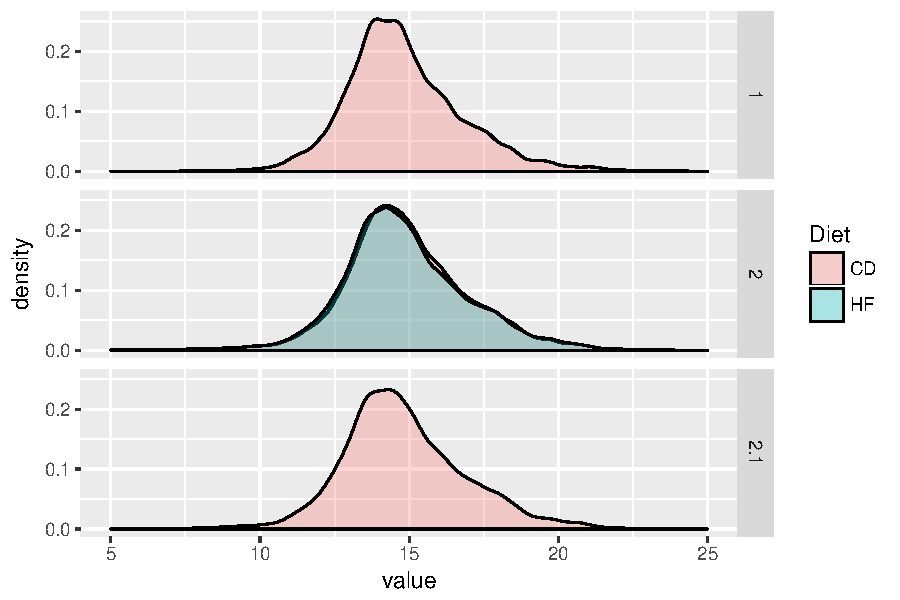
\includegraphics[width=0.7\linewidth]{3.Proteomics/protein_batch_effect_figure.pdf}
     	\includegraphics[width=0.7\linewidth]{"3.Proteomics/Proteomics PCA"}
     	\caption{ \textbf{Top:} Peptide Intensity densities in the three preparation batches colored by diet. Although diet does not significantly effect the peptide quantifications and the preparation does seen to skew the densities slightly. \\ \textbf{Bottom: } PCA analysis of the proteomic data indicates the first two principle components explain 56\% of the variation seen in the data. Unfortunately, the first principle component separates the data based on the batch}
     	\label{fig:Proteomics Batch Effects PCA}
     \end{figure}
          
	The principal component analysis (figure \ref{fig:Proteomics Batch Effects PCA}) of the data shows that large parts of the variation in data come from batch effects, rather than the intrinsic biological heterogeneities between mice. The first two principal components explain 57\% of the variation in the data, the first principle component axis segregating the samples according to their batch numbers. The analysis of the peptides intensity densities between batches shows larger differences than peptides intensity densities across mice on different diets. Similarly, hierarchical crusting analysis(not shown) clusters the mice in batches 1, 2.0 and 2.1 into three distinct clusters. Although batch effects are a problem in proteomics which can be tackled using a range of statistical techniques\citep{Leek2010TacklingBatchEffects}, no such methods of correcting the peptide intensities or correcting p-values generated from statistical tests are used in the subsequent analysis as this data is preliminary.
		

	\section{Proteomics Fold-change Analysis}
	
    \begin{figure}[htb!]
		\makebox[\textwidth][c]{
		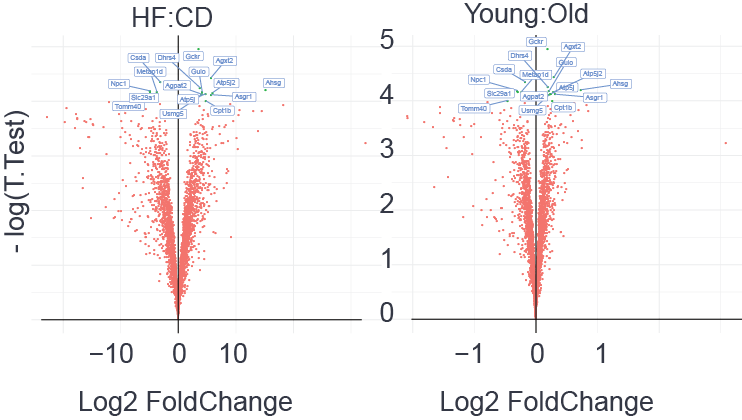
\includegraphics[width=1.2\linewidth]{3.Proteomics/Protein_foldchanges}}
		\caption{Volacano Plots Diet and Age Related Protein Foldchanges}
		\label{volcano plot: Protein Diet and Age Foldchanges}
	\end{figure}
	
	Analogous to the metabolites, there are proteins that have a large fold change in between the diet cohorts as compared to the age cohorts. In fact very liberal fold change threshold have to be set in order to highlighted a few significant proteins in the volcano plot below (figure \ref{volcano plot: Protein Diet and Age Foldchanges}). At the same significance thresholds for diet as age, there are hundreds significant proteins. This speaks to the difficulty performing age-related studies. The effects sizes between the cohorts are not large, and in order to detect the few up or down regulated proteins in old mice, one must be willing to have a very high false discovery rate. In a similar study performed in over 4000 mouse tissues by \citeauthor{Walther2011AccurateQuantification}, minimal age related changes in the proteome were found. 
	

	\section{Protein Biomarkers}
	
    In order to find predictive biomarkers for age, the significance threshold is sequentially lowered to allow 5, 10, 15, 25, 50 and 100 proteins into the biomarker prediction pipeline. 4/5ths the data will then be used to train SVM (support vector machine) and RF(Random Forest) models to classify old and young mice. The n 1/5 validation set will be used to construct confusion matrices and ROC curves to determine the classifier accuracy each method. This is done multiple times, stochastically leaving a 5th the data out for validation. In the end, the factors protein that is chosen most frequently in these machine learning techniques will be used in further QTL and network mining techniques. 
	
	\section{ROC Curves}
	
    ROC(receiver operating characteristic curve) curves originally developed in world war 2 for radar signal detection is a graphical method evaluating the performance binary classifier systems \citep{HajianTilaki2013}. They are routinely used to evaluate classifiers and in the case of this thesis, we are evaluating the prediction accuracy of a SVM and RF classifiers assignments of mice to old or young age cohorts from a small set measured proteins concentrations. A ROC curve is defined as a plot of sensitivity (the number true positive decisions/the number actually positive cases) as the y coordinate versus its specificity(the number true negative decisions/the number actually negative cases) or false positive rate (FPR) as the x coordinate. From the ROC curves, the area under the ROC curve(AUROC) can be computed and used to determine which classifier and ensemble factors are best able to differentiate mice on different age cohorts \citep{HajianTilaki2013}.
	
	\section{Random Forest}
	
    Decision Tree methods are a widely used for classifying large multivariate data. This method is non-parametric and dissects data into segments that start with a root node, and multiple branching nodes terminating in my leaf nodes. At each branch node, the data is segmented into two populations along a variable, this is down hierarchically, moving down the tree until a final classification is declared \citep{Song2015DecisionTrees}. Although tree methods have good interpretability and provide easy intervention options, classification trees use a greedy search algorithm and thus can be unstable to noisy data\citep{Song2015DecisionTrees}. Good prediction results with the diet classifications can be made using tree methods because there are a few very strongly represented molecules in each diet. The age-related classification is not as good as fats(which show large variances and are not well measured) are often selected for partitioning the groups. Moreover, single tree methods are not stable when small sub-samples of the populations of mice (a few strains of interest) are used.
   
   Random forests are an extension of decision tree methods in which a large collection of de-correlated decision trees are built using random sample selection and then averaged \citep{Hastie2009}. For a given set of data, a subset of the data is randomly chosen and a decision tree is generated. Additionally, a random subset of variables in the dataset is used for determining the split points in the decision trees. Many noisy trees are generated from a random selection of data variables and generate an ensemble of classifications. The classification result of each tree in the ensemble gives a "vote" and a classification is made using a majority vote\citep{Hastie2009}.  
   
   The randomForest forest package in R is used to determine in a mouse sample's to determine the most important proteins concentrations for predicting age and diet cohorts \citep{Liaw2015}. Although Random Forests are difficult to interpret simply,\citeauthor{Breiman2001} suggest looking at the misclassification rates in each tree of the out of bag(OOB) samples with and without each variable\citep{Breiman2001}. This means after each tree is generated the OOB mouse samples are classified with and without certain proteins is computed in order to determine the importance of the protein in the prediction \citep{Hastie2009}. 
   
	
	\begin{figure}[htb!]
		\vspace*{-5cm}
		\makebox[\linewidth][c]{
		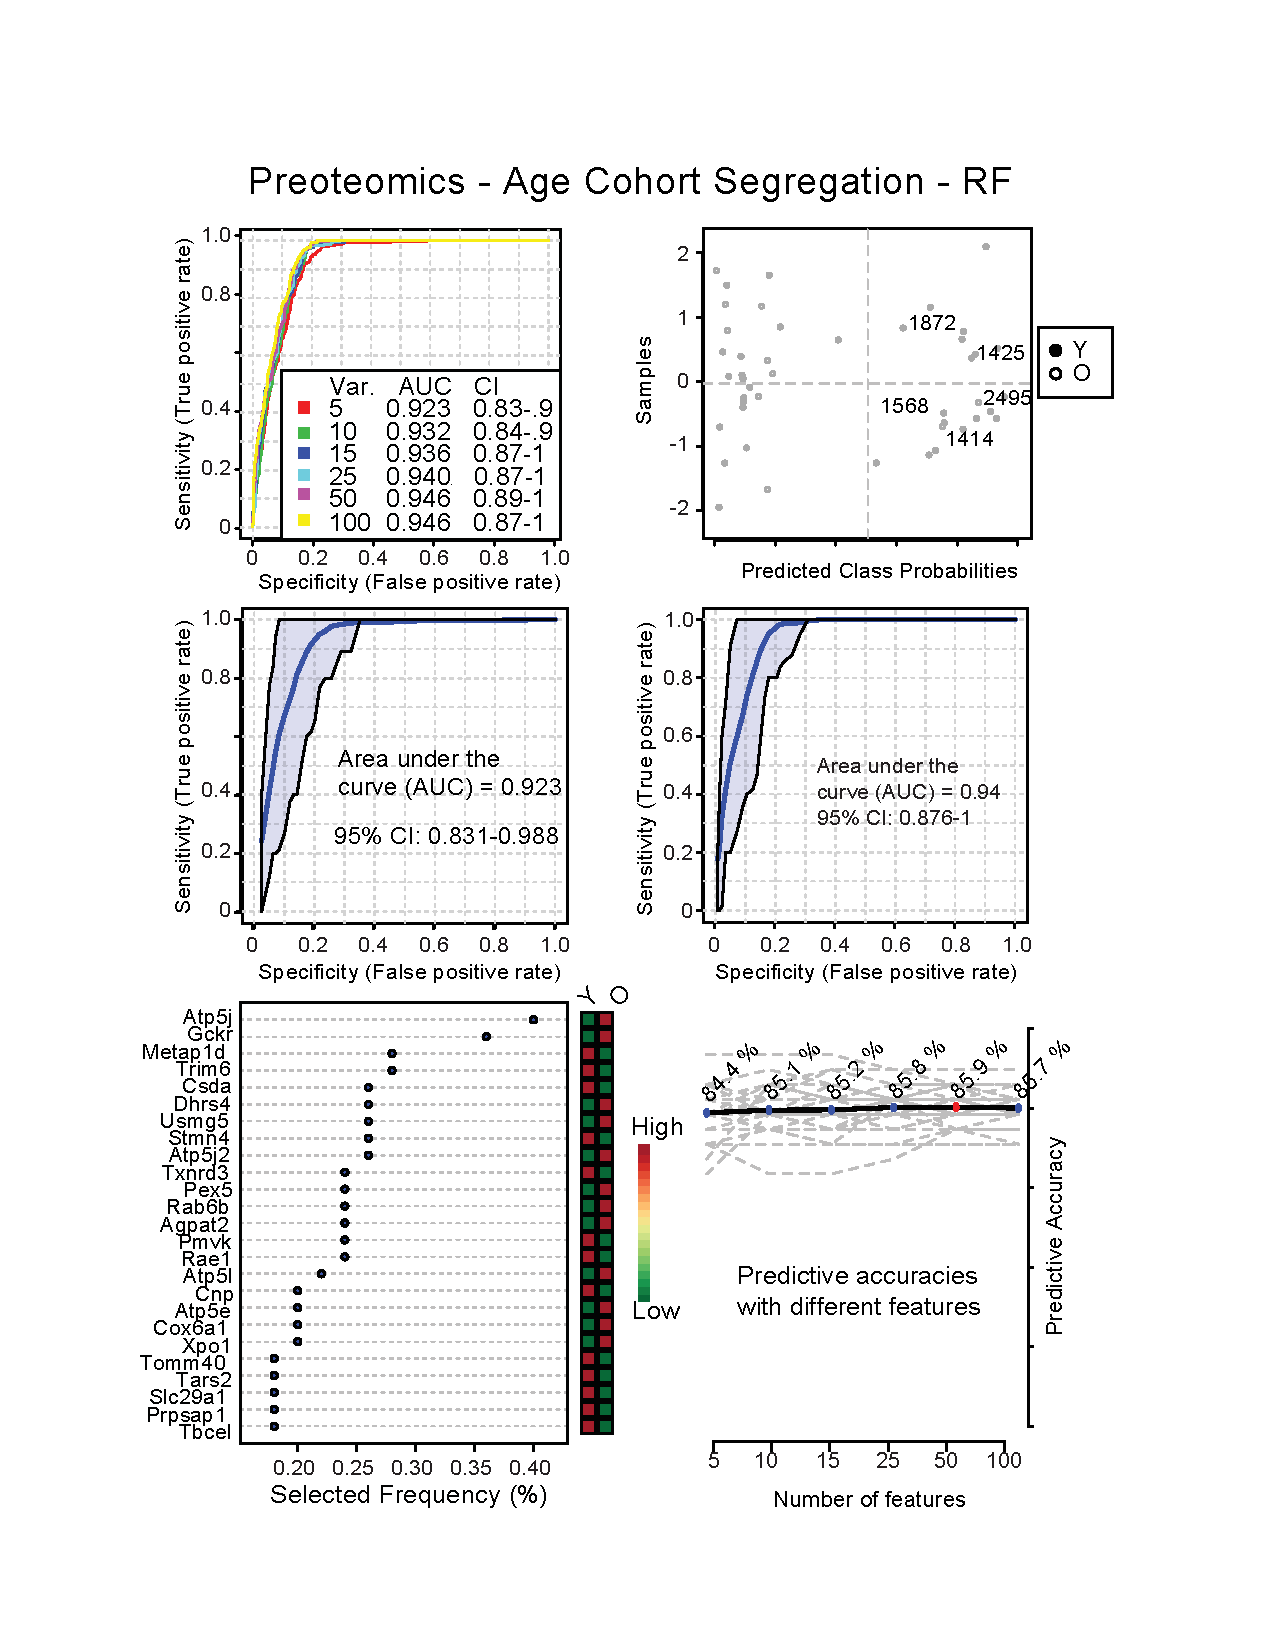
\includegraphics[width=1.4\linewidth]{3.Proteomics/Proteomics_Vingette_Random_Forest_Age}}
        \caption[Random Forest Classifier for Young and Old Mice]{In the top left panel, the ROC curves for various model sizes are given, along with its AUC and the 95\% confidence intervals. In the top right, the Dark and white dots are given in terms their classification probability. In the Middle row, the ROC curves for 5 and 25 proteins are given. In the Bottom left, the most frequency chose factors are given. These factors are seen as prototypic for aging and will be followed up with in further analysis using transcript data. In the bottom right the accuracy for each model size is given} 
        \label{fig:proteomicsvingetterandomforestage} 

	\end{figure}
	
	\clearpage
	\section{Support Vector Machine}
	
	The SVM classifier is similar to older linear discriminant methods. In brief the algorithms attempts to construct the optimal hyperplane that can separate the diet and age mouse cohorts\citep{Shawe-Taylor2011SVM}. The R package rminer is used in this case, with the varaible importance genreatedf rom the Imporatnce function \citep{Cortez2016}.
	
	\begin{figure}[htb!]
		\vspace*{-5cm}
		\makebox[\linewidth][c]{
		\includegraphics[width=1.4\linewidth]{"3.Proteomics/Proteomics_Vingette_SVM_Age"}}
        \caption[SVM Classifier for Young and Old Mice using Proteins]{In the top left panel, the ROC curves for various model sizes are given, along with its AUC and the 95\% confidence intervals. In the top right, the Dark and white dots are given in terms their classification probability. In the Middle row, the ROC curves for 5 and 25 protein are given. In the Bottom left, the most frequency chose factors are given. These factors are seen as prototypic for aging and will be followed up with in further analysis using transcript data. In the bottom right the accuracy for each model size is given} 
		\label{fig:proteomicsvingettesvm}
	\end{figure}
	
	
	\section{Conclusions From Proteomics}
	
    In this section, a small 22 mouse subset the 631 mice were analyzed using SWATH-MS. The protein quantification data that was put forth had many significantly different proteins for the different diet cohorts but very few significantly changed proteins in different age cohorts. As a result, SVM and RF methods were used, producing very good classifications of whether the mice were young old on the basis 5 to 100 proteins. Although the interpretability of these algorithms is difficult, one can try to look at overlaps between common proteins selected across both SVM and random forest and perform QTL analysis in the future. The number of samples analyzed is extremely small in relation to all the other BXD proteome data that will be quantified in coming experiments. The preliminary proteins hit found here are used with the metabolite data and transcript data to try to construct age-related protein network. 
	
	\chapter{Transcriptomics}
	
	\section{Introduction to Micro-arrays}
	
    Preliminary transcript data from 99 mice was also produced using Affymetrix microarrays. These microarrays are silicon substrates that have a library of known cDNA fragments immobilized to their surface in discrete pixels \citep{Miller2009MicroArrays}.  Experiments profiling the expression and relative abundance of a large set transcripts can be performed in a piece-wise manner. All of the transcripts in samples are functionalized with a fluorescent tag and introduced on to the surface of the microarray. When transcripts hybridize with complementary cDNA on the chip, the fluorescence intensity read off the chip using a charge-coupled device(CCD) camera is proportional to the concentration of the tagged transcript. Fluorescence standards on the chip seen in the red outline in figure \ref{fig: Zoomed-in Photograph of a Microarray} used to convert florescence throughout the chip into concentrations. Sometimes, the CCD camera can image certain parts the chip slightly lighter or dark, systematically biasing the measurements in segments of the photograph. The green box shows intensity normalization pixels that are placed throughout the chip in order to correct against irregularities in the CCD. 
	
	\subsection{Transcriptomics Data Processing}
	\begin{figure}
		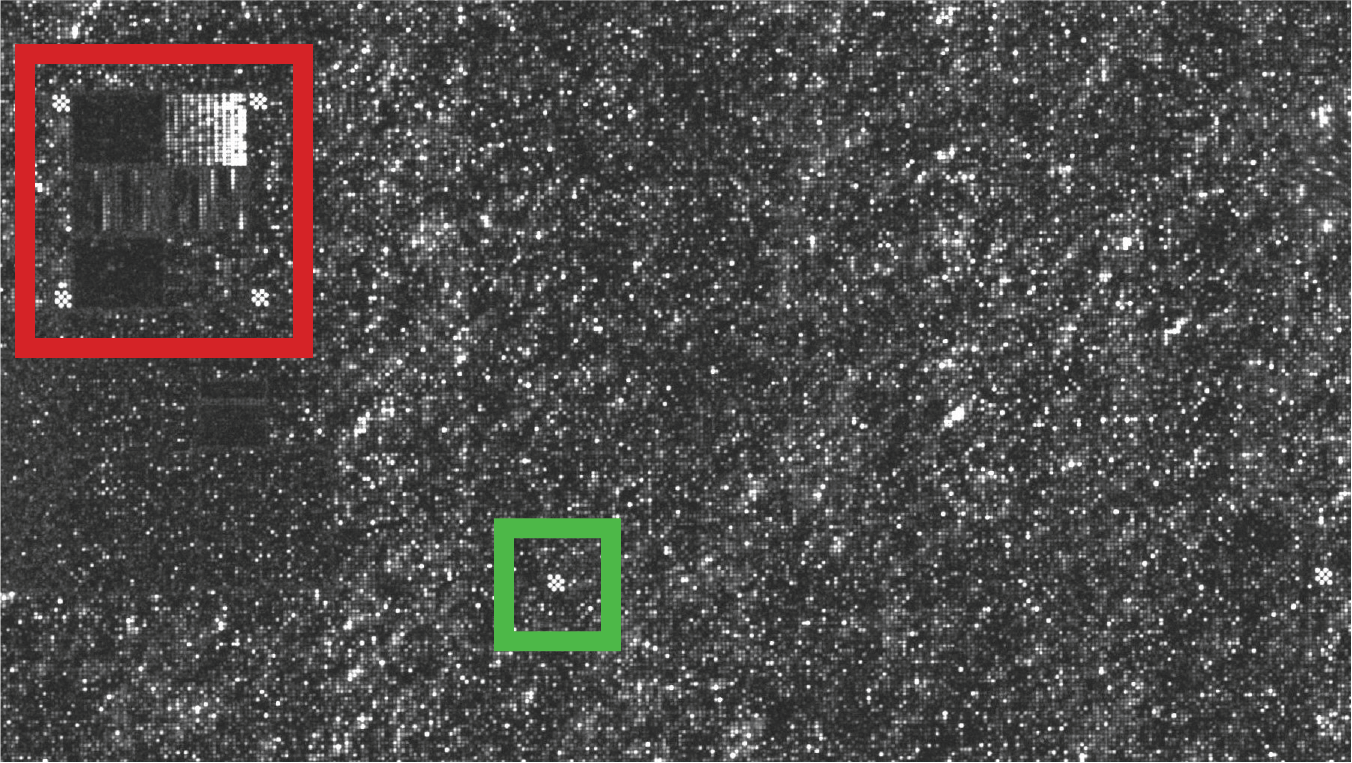
\includegraphics[width = 1.0\linewidth]{3.Trancriptomics/Affimetrix_Chip_ZoomIn.png}
		\caption{A zoomed in picture of a micro-array that can be processed to determine transcript levels. This is a one color array meaning single sample intensities are given. The red box is surrounding the intensity standards that are used to calibrate the intensity to transcript concentration ratio. The green box is around an intensity marker which is used to normalize the intensities across the chip irrespective defects that may capture different parts the chip with lower or higher intensities}
		\label{fig: Zoomed-in Photograph of a Microarray}
	\end{figure}
	
    Microarray experiments were not performed in-house. instead, the BXD mouse liver tissues were frozen in $N_(2l)$ pulverized to a powder in a motor and pestle and shipped to the United States for processing. At the facility, RNA is extracted from the mouse livers using the TRIzol® Plus RNA Purification System \citep{Rio2010TRIzol}). It is converted to cDNA and fictionalized with a fluorescent tag before microarray analysis is done. The raw unprocessed DAT, CDF, and CEL files were returned for analysis using RMA express and R.
	
	
	\subsection{Data Extraction} 
	
    Microarray expression data can be extracted with two files, the CDF, and CEL files. The CDF (Chip Description File) contains information about the probes on the gene array chip \citep{BenBolstad2003}. One CDF is required for all 600 mice in the full experiment because the layout of the probeset is the same for every mouse transcriptome being profiled. For each gene being profiled on the chip, there is a set of oligonucleotide probes 25 nucleotides long that are used to determine its transcript expression. As it is difficult to predict whether a probe will efficiently bind to its target, a probe set contains both a perfect match probes that have the identical sequence of the gene and mismatch probes that have a substitution in the central nucleotide of the probe \citep{Liu2010}. Mismatch controls should always show lower intensity than the perfect match probes and they sets are placed in different parts of the chip and quantify the amount of cross-hybridization that occurs from non-target genes. The CDF file also contains the location of control probes that can be used to correct of heterogeneities in the CMOS image detector across the gene array \citep{BenBolstad2003}.   

	The pixel intensity values that are detected at each spot on the gene array are saved in an efficient DAT format \citep{Miller2009MicroArrays}. For an initial inspection, the DAT file can be open in an image viewer such as photoshop to ensure positive control show high intensities through the chip and that there is no smears or local aberrations in the light intensity, possible introduced form mishandling of the chip. This format, however, is difficult to work with so DAT files are converted to CEL files. The CEL file thus stores the results the intensity calculations on at each pixel that is extracted from a DAT file and interface are readily accessible with other bioinformatics tools for analysis \citep{AffymetrixInc}.

	RMAExpress reads in the pixel intensities in the CEL files and the probe information in the CDF files can return a table of normalized or raw intensities for each gene \citep{BenBolstad2003}. This software is used as an alternative to using R packages like affy to perform this, the simple graphical user interface is used load in the data and conveniently export it easy to use formats. In this study, RMA expressed is used to generate a CSV table of all transcripts and their intensities. Normalization and model-based background subtraction are done in R in accordance with model-based approaches found in \citep{Irizarry2003,Irizarry2003a,Bolstad2003}.

	\subsection{Normalization}
	
    In experiments deploying multiple high-density oligonucleotide arrays, there are a number of technical factors involving the imaging and data processing and the thermodynamics that govern the nucleotide binding that can contribute signal variation that does not have a biological origin\citep{Bolstad2003}. Normalization of the signal intensities can reduce the non-linear relationship between the concentration of nucleotides and the detected intensity of the pixel on the chip. Using a model-based approach that incorporates an understanding of probe binding can generate normalized results much better than the standard normalization provided by standard Affymetrix software \citep{Bolstad2003}.
	
    Many traditional statical methodologies such as t-tests which will be performed on the microarray data afterward are based on the assumption normally distribution or at least symmetrically distributed data, with constant variance. if the assumptions are violated, finding that are determined are significant may just be the results of statistical errors. All the following model based normalization techniques are adapted from \citep{Durbin2002}.
	
	\subsection{Model Based Error Subtraction}
	An error model is required to remove the non-biological noise from the system. in our model we assume 
	
	\begin{align*}
	\text{if : }  & x_ki & \text{is the true abundance the probe k in sample i} \\
	\text{if : }  & y_ki & \text{is the measured intensity on the micro-array} \\
	\text{then : }  & y_ki = a_ki + b_ki * x_ki & \text{If we assume true abundance is proportional to signal intensity}
	\end{align*}
	
	In the equation above, we assume the signal detected is a function the abundance the transcript in addition to noise that depends on the abundance and also noise that is independent or systematic noise. The parameter $b_ki$ summarizes abundance-dependent noise: which includes number cells, hybridization efficiency, label efficiency. The parameter  $a_ki$ Summarized the abundance-independent noise. This noise can arise from unspecific hybridization, background florescences that may have been detected or stray signals. 
	
	If we assume only multiplicative noise in the linear model above and assume all the noise in the measure is derived from abundance-dependent noise. 
	$$ Y_ki = a_ki + b_ki * x_ki $$
	$$ a_ki \approx 0 $$
	$$ b_ki = b_i \cdot\beta $$
	$$ b_ki = b_i\beta_k(1+\epsilon_ki) $$
	
    The concentration-dependent parameter $b_ki$ is then composed the sample-specific noise which is described by $b_i$ and the probe specific noise given by $\beta_k$. The remaining noise is modeled with a stochastic portion the model. In end the final model taking into account the multiplicative noise only can be given as:
	
	$$ Y_ki = b_i\cdot\beta_k{\cdot}x_ki ( 1 + \epsilon_ki) $$ 
	where $ \epsilon_ki ~ Norm(0,c^2)$ and c is the coefficient variation as defined by $c = \dfrac{std}{mean}$
	
	With this formulation, if we want to determine the relative abundance a transcript with respect to another we can use the expression
	$$ M_k = \dfrac{Y_{k2}/Y_{k1}}{b_1/b_2} $$
	
	In the more natural case we can assume the existence both multiplicative and additive noise and in this case our linear expression for determine the true abundance the transcript must be slightly altered. The additive noise term is also composed a systematic error term $a_i$ and sample specific but abundance-interdependent term $b_i\eta_{ki}$. 
	
	\begin{align}
	Y_ki = a_ki + b_ki \cdot x_ki && a_{ki} = a_i + b_i\eta_ki && b_ki = b_i\beta_k(1+\epsilon_ki)
	\end{align}
	
	this yields the final model given below: 
	$$\dfrac{Y_ki - a_i}{b_i} = b_i\beta_k^{\epsilon_ki} + \eta_ki$$
	
	\begin{center}
		where $\eta_ki ~ N(0,c^2)$ and $\epsilon_ki ~ N(0,s^2) $
	\end{center}
	
	This equation allows us to model all the sources noise in the micro-array data from defined endogenous and exogenous sources in order for us to subtract it of, as indicated int he $Y_{ki} - a_i$ term. 
	
	\subsection{Variance Stabilizing Normalization}
	
	\begin{figure}[ht]
		\makebox[\textwidth][c]{
		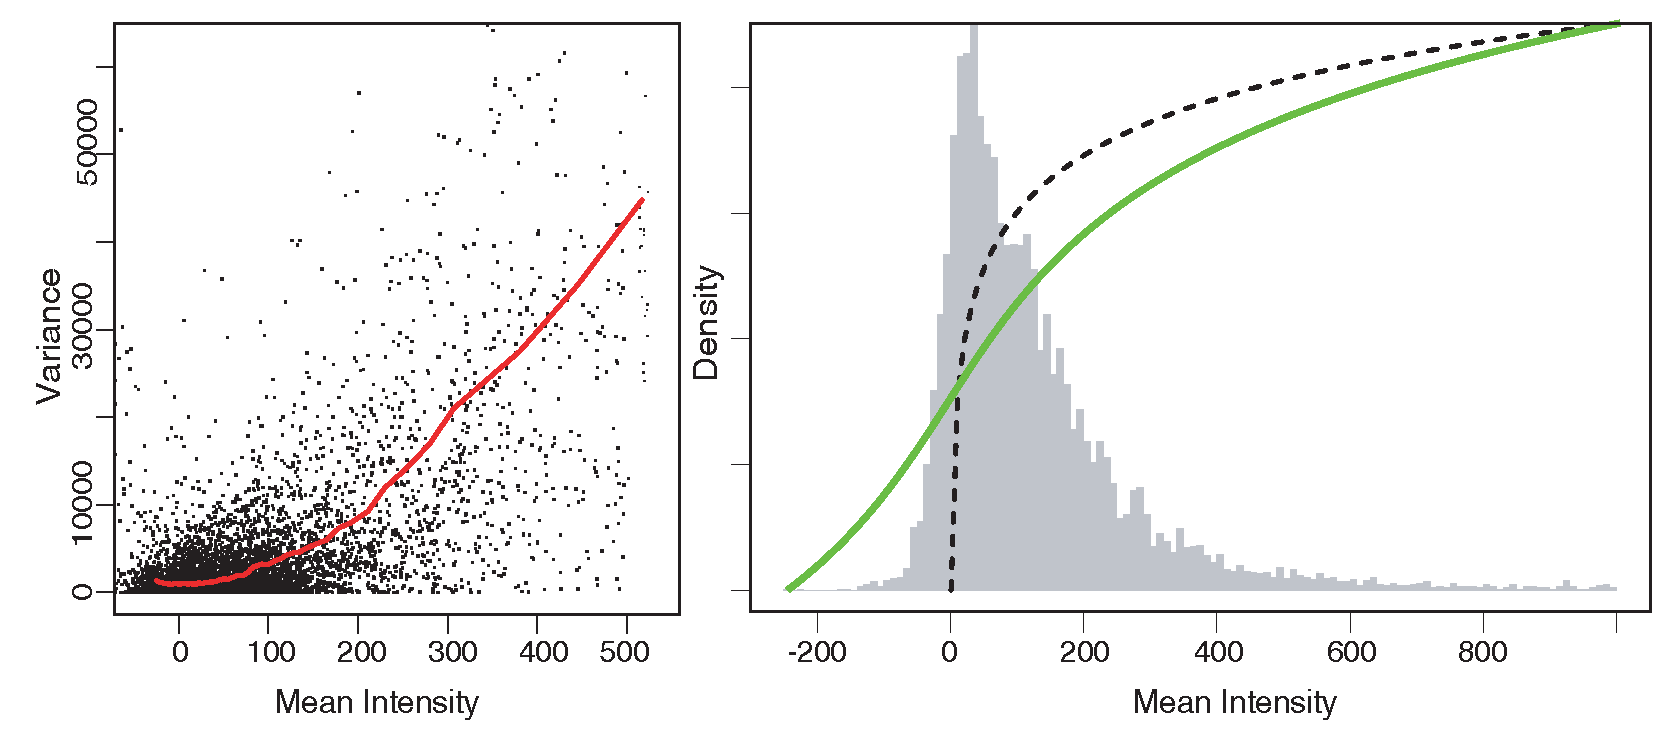
\includegraphics[width=1.2\linewidth]{3.Trancriptomics/Variance_stablizaiton.pdf}}
		\caption{Adapted from  \citep{Durbin2002}.(Left) The variance and mean relationship found in experimentally produced microarrray data. The red line shows a plot the v(u) described in at the end section 2.3.6(right) The variance stabilization transformation performed on the data. The green line represents a log transformation, and the dotted line the arcsinh transformation which is hte preferred transformation method   }
	\end{figure}
	
	Although the background noise has been subtracted a variance stabilization still needs to be performed on the data. This is because the coefficient variation is not constant throughout the dataset.  \citep{Durbin2002}. There is a quadratic relation between 
	$v = var(Y_{ki}$ and $u = E(Y_{ki})$
	$$v(u) = c^2(u-a_i)^2 + b_i^2s^2$$
	
	this relationship can be shown using empirical data. The figure below shows variance and expected values plotted against each-other illustrating the quadratic relationship. From visual inspection it seems a log transformation may benefit the micro array data, it is not obvious which transformation is optimal for stabilizing the variance in our data. \citep{Durbin2002}.  Since the log transform is not defined for values under zero, values that become negative after the background subtraction are not defined, forced us to throw out large swaths data. Moreover, a log transformation provides good variance stabilization at high levels, but inflate the variance close to the detection threshold. \citep{Durbin2002}.  Therefore, an arcsinh transformation is used instead as it behaves like the log transformation asymptotically but is linear in the lowest intensity regions.
	

	
	The variance stabilization transformation used with out micro-array data is then
	$$h_i(y_{ki}) = arcsinh(\dfrac{c}{s}{\cdot}\dfrac{y_{ki} - a_i}{b_i}) $$
	
	\begin{minipage}{\linewidth}% Following stays together
		The final result this transformation is that intensities are normally distributed with a constant variation $c^2$ and a mean $b_i\beta_k$. Now if we would like to quantify differential expression we can use the expression
		$$ {\Delta}h_{k,ij} = h_i(y_ki) - h_j(y_{kj}) $$
	\end{minipage}
	
	
	\subsection{Parameter Estimation}
	
	In the end the final model used to perform the variance stabilization with out expression data is
	$$ arcsinh(\dfrac{y_{ki}-a_i}{b_i}) = b_i\beta_k + \epsilon_{ki}, \epsilon_{ki} \sim N(0,c^2)$$
	
	In order to fit the parameters, one can use a maximum likelihood estimation. The model parameters can be fitted by using the majority genes unchanged assumption in which the sample specific noise parameters can be more or less assumed to be the same across all transcripts. 
	$$ b_i\beta_k = b\beta_k $$
	$$ arcsinh(\dfrac{y_{ki}-a_i}{b_i}) = b_i\beta_k + \epsilon_{ki}, \epsilon_{ki} \sim N(0,c^2)$$
	
	
	\section{Quality Control}
	
	\begin{figure}[htb!]
		\makebox[\textwidth][c]{
		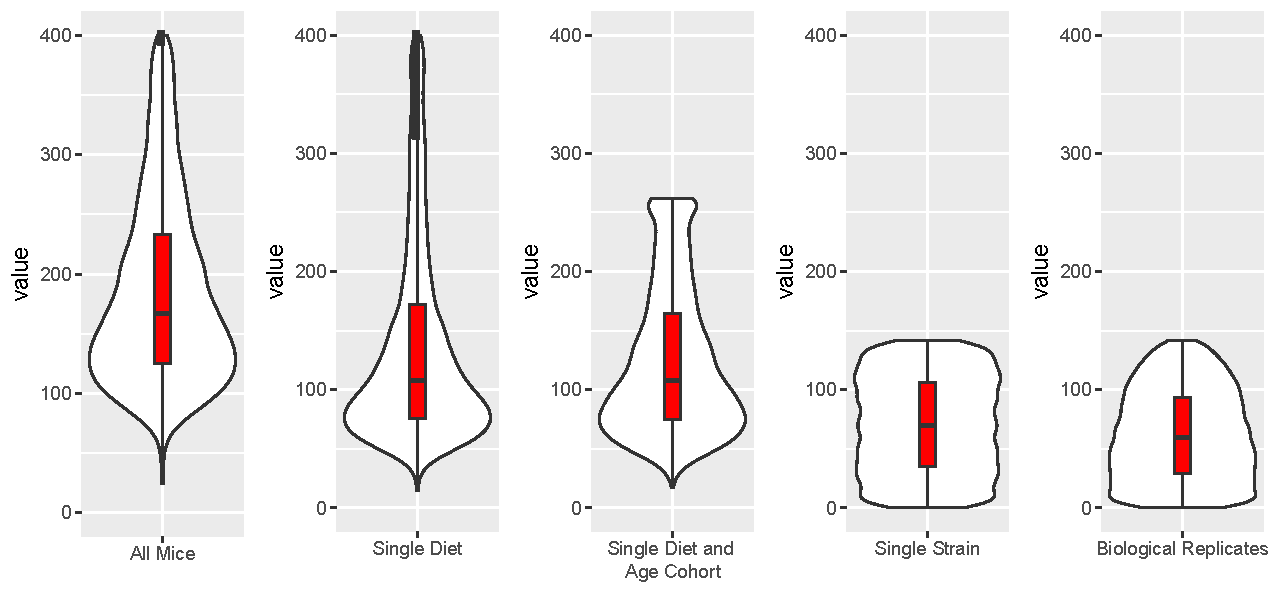
\includegraphics[width=1.2\linewidth]{3.Trancriptomics/transcript_CV_figure}}
		\caption{CV Analysis of Transcript Data}
		\label{fig:transcriptcvfigure}
	\end{figure}
	
	The coefficients of variation in the RNA data are as much larger than those seen in the protein and metabolites. This due to the many order of magnitude over which different transcripts can be produced. The biological replicates themselves show nearly a 100\% coefficient of variation indicating large fold changes are needed to reliably detect differences in the transcription between mouse cohorts. 
	
	\subsection*{Tissue Contamination}
	
    One of the biggest challenges with analyzing transcriptomics data from organs or samples containing more than one cell type is the effect of variations that come from changing proportions of cell types within each sample. Although liver is a large relatively homogeneous organ, overwhelmingly made up of hepatocytes, there are also a range of endothelial cells which make up parts of the vasculature that supply blood to and from the liver, it and a host of invading immune cells that are present in almost all tissues irrespective of the inflammation state of the animal. All of these cells that influence the gene expression patterns independent of the effects being studied and may lead to a perceived enrichment of certain gene pathways, when we are simply assaying different cells. This is a complication encountered in this study because specific lobes of the liver are not always used for the same omics analysis, instead, the livers are ground in liquid nitrogen, with the resulting powder being partitioned into many aliquots with slightly different portions of each lobe. 
	
	\begin{figure}
		\centering
		\includegraphics[width=1\linewidth]{3.Trancriptomics/BioQCPoint.png}
		\caption{BioQC data showing the organ classes the BXD mouse samples are mostly to come from. Most sample show high liver signatures, however there is evidence for a high degree of immune cell infiltration in many samples}
		\label{fig:bioqcpoint}
	\end{figure}
	
    BioQC is a package developed at Roche that quantifies samples based on their resemblances to organs and provides a quantitative method with which to determine the context of samples and their comparability \citep*{Zhang2017}. This package uses manually curated gene signatures that are prototypic for 150 tissues types or organs, and in some cases, a an organ in a single development state (embryonic and mature kidney have varying transcript levels in many genes) which are used determine organ scores for each sample. This method has the distinct advantage over unsupervised learning techniques like PCA which can be used to visualize and manually inspect the distance between two samples but does not show the source of the contamination \citep{Zhang2017}. As can be seen in figure \ref{fig:bioqcpoint} in the BXD mouse samples, all of the liver samples have high mature liver scores above 80 followed by intermediate embryonic liver scores and lower scores for adipose tissue and monocytes which make up minority constituents of the samples. The two mature liver scores were given, Liver NGS, which is derived from the RNAseq Atlas\citep{Krupp2012}) and Liver NR, derived from an in-house Roche liver panel, show similar results with concomitant drops in scores for samples 18, 33, 62 and 80. The Liver NGS score is more specific to humans and gives lower scores as compared to liver NR. 

	Overall, one can conclude a low amount of contamination for the expectation of four samples in the first 96. In the heat-map visualizing the same data(figure \ref{fig:bioqcheatmap}), one can see the large areas of dark blue indicating low BioQC scores for cell types such are brown fat and microglia. One sample, 62 does not have any organ enrichment score, indicating technical error or errors in handling and preparing the sample. The other samples can be roughly grouped into two categories of liver cells. The minority group which have lower liver scores using the Roche and NGS panel on average and have high scores for immune cells like macrophages, granulocytes, and lymphocytes. Immune cells surveillance is well documented in the liver, as portal circulation brings disgested material from the intesnites directly to the liver where it can act as a frontline defense for materials entering circulation to the rest of the body\citep{Jenne2013}. These mice most likely have an infection or have been exposed to something that contained immunogenic material. The rest of the samples show very high liver scores, meaning there has high expression of genes that are expressed in normal human liver. 
	  
    \begin{figure}[htb!]
    	\centering
    	\includegraphics[width=0.9\linewidth]{3.Trancriptomics/BioQCHeatmap.png}
    	\caption{Heatmap of BioQC scores for the 96 samples. Most of the samples show high BioQC scores indicating, genes known to be expressed selectively in liver are detected in most of samples. BioQC scores for immune cells are also detected, indicating the presence of infiltrating cell in the samples as well}
    	\label{fig:bioqcheatmap}
    \end{figure}
    
	\section{Transcript Level Fold Changes}
	
	\begin{figure}[ht!]
		\makebox[\textwidth][c]{\includegraphics[width=1.3\textwidth]{3.Trancriptomics/VolcanoTranscrpt}}
		\caption{Volcano Plots Diet and Age Cohort Fold Changes}
		\label{volcano plot: Diet and Age related Transcript Foldchanges }
	\end{figure}
	
    In a dramatic reversal from the proteomic and metabolomic data, the transcript data is highly enriched with differentially expressed transcripts between older and younger mice. Much like the proteomic data, too many hits are found using the a of 0.05 threshold for significance and a 1 fold log fold2 change. Such a large set of traits can be difficult to follow up with literature reviews and QTL analysis. As such all of the transcripts enriched in the old mice, are added to networks previously used to investigate metabolites and protein data. The goal for this integrated analysis is to determine causal circuits for the certain metabolite concentrations in the liver.
	
	As an initial look at the relationship between the three layers information we have, one can look at the correlation between proteins and transcripts and realize that they are not very tightly coupled. For the few very highly correlated sets protein and transcripts, many are metabolic genes such as hexokinase. From this one can conclude that even though not all pairs protein and transcript will be instructive and add an explanatory information for certain metabolites levels seen, they may be in a small subset of metabolites.  
	
	\begin{figure}[htb!]
		\centering
		\includegraphics[width=\linewidth]{3.Trancriptomics/Protein_RNA_COrr}
		\caption{Correlation Coefficients between protein and RNA}
		\label{fig:proteinrnacorr}
	\end{figure}
	
	\section{ Gene Set Enrichment Analysis }
	

    An efficient way to determine which pathways of interest may be enriched between mice of different ages diets is the use of gene set enrichment analysis(GSEA). In this study webgestalt is used to perfrom this enrichment analysis \citep{Wang2017}. Genes that are known to be involved in certain processes such as primary metabolism or cell proliferation are curated into a biological process, organelle and molecular function sets that be used to interpret a set of given genes. In the BXD mouse data, there are many differentially expressed gene across the diet and age cohorts but the processes of the genes that are differentially expressed as quite similar indicating, that it may be difficult to disentangle the effects of age and diet without looking at intersectional sets such old/HF mice vs. young/HF mice, as compared to just doing a wholesale comparision between diets or age cohorts. 
    
    \begin{figure}[hbt!]
    	\centering
    	\includegraphics[width=\linewidth]{3.Trancriptomics/GSEA}
    	\caption{Gene Set Enrichment analysis results for the top 263 genes that are differentially expressed across age \textbf{left} and across diet \textbf{right} }
    	\label{fig:gsea}
    \end{figure}
    
	\subsection*{Genes involved in Metabolic Processes}
    When comparing gene expression across mice in different diets, 8 more genes involved in metabolic processes seem to be enriched as compared to genes differentially expressed in the aging cohorts. This can be attributed to the differences in the enzymes required to process components of two diets. In the age cohorts, there are roughly equal numbers of mice in either diet and these differences are difficult to detect. For example, pancreatic colipase, carboxyl ester lipase, and pancreatic lipase are all genes that are up-regulated in mice on the HF diet and help the breakdown of fatty acids and acyl esters that are enriched in the HF diet.  Additionally, there is an increase in genes such as hydroxy-delta-5-steroid dehydrogenase involved with steroid metabolism which may be expressed to process an analogous increase in serum sterols as fatty acids in the mice. The upregulation of these genes is corroborated with the high expression levels of these proteins in the HF diet mice. Although the coupling of the transcript levels is again, not high across all of the lipid processing genes, it is above the average correlation coefficients for all proteins with their transcripts.

	Interestingly, as mentioned before, partial oxidation of fatty acids may be a hallmark of aging in mice and may be the source of oxidation stress in older mice can be seen in our transcriptomics data. A number of genes that are involved in fatty acid metabolism are differentially expressed in older mice. This includes a host of Cyp genes, such as Cyp2c69, Cyp2b13, and Cyp2b9 and hydroxy acid oxidases, acetyl-Coenzyme A acyltransferases and fatty acid desaturase which are enzymes involved in the processing of impartially digested fatty acid derivatives \citep{Voet2011Biochemistry}. Additionally, the contingent of metabolic processes that are differentially expressed genes between old and young mice also include gene for purine and nucleoside metabolism such as guanidinoacetate methyltransferase and galactose-1-phosphate uridyl transferase which generate nucleotides and catalyze reactions that produce the substrates for DNA replication and are thus related to the cell cycle and aging process \citep{Voet2011Biochemistry}. 
	
	\subsection*{Gene involved in Response to Stimuli}
	
    Genes that are involved in the response to stimuli are genes that ameliorate the effect of chemical and physical phenomena that can perturb normal cellular function such as oxidation stress and radiation. As a confirmation to the previous hypothesis that oxidation stress and oxidized glutathione accumulated in older mice, there are a handful of genes including glutathione peroxidase 3, glutathione S-transferase, theta 1 and myeloperoxidase which are all enriched in the older mice. In the older mice, the effect of radiation damage accumulation can also be seen in the upregulation of cell cycles genes like cyclin-dependent kinases and genes involved in repair double-stranded breaks in the DNA. 

	In the two mouse diet cohorts, accumulations of acid ketone bodies and other fatty acids can be the source of lower blood ph in the animals. As a response to this, the mice on the fatty diets have increased expression of genes such as the inhibitor of DNA binding 3 which is involved in the response to acid chemical and acidosis \citep{Wang2017}.
	
	\section{ Multi-Omics Data Integration }

	\begin{figure}[hb!]
		\centering
		\includegraphics[width=\linewidth]{3.Trancriptomics/Integrated_Linoic_Acid}
		\caption{Integrated analysis of Linoleic Acid Oxidation}
		\label{fig: Integrated Model of Linoleic Acid Oxidation}
	\end{figure}

	\subsection{Integrated Analysis of Linoleic acid Oxidation}
    As an initial proof concept to show that proteins, metabolite and transcript data could be used together to generate causal networks, a small part of the Linoleic acid metabolism was modeled (figure \ref{fig: Integrated Model of Linoleic Acid Oxidation})    In the first reaction phosphatidylcholine is cleaved by Pla2g12b into linoleic acid. The metabolites, protein, and transcript are all similarly expressed. When the fatty acid has become linoleic acid it can be converted by various lipoxygenases and cytochrome p450 enzymes into either 12,13-epoxide, Vernolic acid or the  9,10-epoxide, Coronary acid. The regulation of this circuit is known in \textit{Vernicia fordii)} where the genes that increase production of the oil experience product repression \citep{Li2010Vernonia}. Data from the effects of these oils in terms of its substrate or product interactions with proteins in mammals is not known. The Cyp genes performing this latter transformation are down-regulated 40\% in high-fat diet mice compared to the chow diet mice and the transcript is unregulated which is in contrast to findings elsewhere on the effect of high-fat diets on cytochrome proteins, drug transporters \citep{Ghose2011HFD}. The lower amount protein may be due to the accumulation the 9-10-epoxide. Although in this toy example, one cannot definitively say that the 9-10-epoxides is down-regulating its catabolic enzymes, as in a Trp repressor type circuit, it is only a hypothesis, one can test once all the layers molecular data are available. 
	
    The metabolite fold changes overall in the pathway, however, are not large enough to rule out chance fluctuations in the relative abundances of any of the biomolecules. Even though there is a 5 fold enrichment of Pla2g12b in the HF diet mice, there seem to be no large changes in the ratio of PC(18:0) and Linoleic acid. Another reason for the lack of difference between up and downstream metabolites in this pathways is that all three of metabolites have multiple isobars. In this case, it is impossible to determine the exact location of the fatty unsaturations which are important in determining the function of metabolites. This and the exclusion of shunt pathways in this rarefied models make it difficult determine the exact reason the large enzymatic fold change does not translate into a large flux through the pathway \citep{Saa2016}.
	
	
	\subsection{Integrated Analysis of Tyrosine Metabolism}
	\begin{figure}
		\makebox[\textwidth][c]{
		\includegraphics[width=1.1\linewidth]{3.Trancriptomics/Integrated_Tyrosine_protein}}
		\caption{Integrated analysis Tryptophan metabolism}
		\label{fig:integratedtyrosineprotein}
	\end{figure}
	
	
    In a slightly more complex example, we can consider the tryptophan metabolism which had was a significant effect pathway in the metabolite data, pathway enzymes were unregulated in the high fat diet in proteomic analysis and transcripts related to those proteins were hits in stringent fold change analysis for transcripts. The central metabolite, L-tryptophan is highlighted in the graph with a deep purple border cannot be produced endogenously and needs to be obtained from the diet. From the central L-tryptophan amino acid, tryptamine, Oxitriptan or L-Formylknynurenie can be formed shuttling the metabolite into three distinct directions, one of which is the production of serotonin and melatonin. Serotonin is synthesized via tryptophan hydroxylase, which converts 5-hydroxytryptophan (5-HTP) into serotonin. \citep{Schaechter1990,Fernstrom1983} . Melatonin is generated from serotonin, via N-acetyltransferase and 5-hydroxyindole-O-methyltransferase activity \citep{WURTMAN1969}. Despite this, it is difficult to alter the level of tryptophan in the tissue ( and as a result the flux of this pathway) from changing an animal's diet as it is brought in by transporters that also transport other competing for amino acids \citep{Robinson2009}. This may be the reason, the integrated analysis was not able to find genetic factors that control the liver tryptophan concentrations. If the effects of the transporters on the concentrations of tryptophan and its cognate metabolites are much larger than any of the effects of mutations in the enzymatic pathways, it may not be possible to determine.
	
     Despite the effort, the that has gone into reconstructing the pathway, including significantly enriched transcripts, proteins, and metabolites in the tryptophan metabolism, definitive conclusion about the direction and nature of the interaction between the layers of biomolecules could not be reached. The issue in this circuit is that the networks fold changes are highly counter-intuitive. One partly interpretable section this network is the reaction, in which melatonin is produced through the reduction of 6-hydroxy-melatonin by a Cyp enzymes. In this case, the lower levels the enzyme and high levels of the product can be interpreted in two ways. Either the production the enzymes are being inhibited by the excess product (which it is, no specific decrease in the transcript between the diets can be detected) or that the Cyp gene is expressed lower on average in the high-fat mice and the 6-hydroxy melatonin is building up due to the low expression of the catalyzing protein.
	 
     For most of the other graph, the inability to put discrete barriers on the reactions thus does not allow us to accurately predict what the causal structure. Moreover, imposing such barrier would be helpful as a theoretical exercise but would not represent the true intermingled nature the metabolism. Moreover, one may look at the large boxes drawn for Ddc, a high overexpressed transcript in HF mice, Aldh3a2 or Haao, another two proteins that are also highly expressed in the HF mice, don't actually seem to have an effect on their downstream metabolite molecules. 
	
	
	\section{Transcriptomics Conclusion}
	
    A large number differentially expressed transcripts in aging mice were found, in contrast to the proteomic data in which there were almost no differences between the age cohorts. Despite having only 22 proteomic samples and 90 transcriptomics samples, detailed descriptions of metabolic pathways with protein and transcript nodes overlaid were generated. The large amount information generating a network diagram can condense is very convenient for visualizing inputs and outputs of pathways. The construction of the aforementioned networks, however, does not allow for easy structural hypothesis testing, as the boundary conditions for the networks are not well defined.
	
	\chapter{Conclusions and Future work}
	
    In this thesis, a large amount metabolic, proteomic and transcriptomic data was collected on 88 strains of BXD mice. The summary statistics for all three of these molecular phenotype readouts can be found in the Appendix \ref{Appendix: Summary Statistics of Metabolite, Protein and Transcript Data}. 

	QTL analysis of metabolites elucidated three strong mQTLs, one for pyruvate, hydroxybutyric acid and glutathione of which glutathione looks promising as a potential target to follow up with using glutathione oxidase inhibitors or recombinant mice with mutant alleles for this gene. There were many other metabolites that had weaker but almost significant which can also be followed up with if the transcriptomics and proteomics data in the pathway of the metbolite looks promising. The search space for enzymes we can interfere with should however, be limited to those enzymes that have large equilibrium constants and are most likely binary switch point for metabolic flux through pathways and are likely to show large effect sizes in reductive validation experiments \citep{Voet2011Biochemistry}. 

	The protein biomarker analysis used in this thesis may have limited support from biostatisticians as the field of determining the most important features for any giving classification algorithm is an area or rapid development and was not investigated in depth in this thesis \citep{Hastie2009}. The proteins found using the feature importance in SVM and Random Forest selection frequency were involved in pathways detected both on the metabolites and transcript level meaning they can be at least used for preliminary validation until more robust methods are deployed.

	The preliminary SWATH results indicate some promising follow up proteins. Once the full SWATH MS and transcriptomics data are produced, more thorough network analysis can be done to determine pathways adversely affected by aging. With less than 100 samples, it is difficult to confidently detect foldchanges, especially in the transcriptomics data where the CVs between biological replication is 50-100\% and any claim as to the up and down regulation of a protein or the reversal of the flux of metabolites through its pathways due to a fold change in the transcript level may be erroneously detected. 

	Once the transcriptomics and proteomics with a larger number of mice completed, it will also be interesting to see if eQTLS and pQTLs can be found in overlapping regions in order to generate a single multilayer QTL that illustrations the full flow of regulation from the gene level up the metabolite. This is very much an ideal case is it can be shown from the preliminary with the linoleic acid and the tryptophan pathways, the data from the metabolites, proteins, and transcript do not always correlation in the ways one would expect. 

	Lastly, the layer by layer analysis performed in this thesis should also be done going in the opposite direction. In principle, metabolites that were differentially representative in their of the diet of the age cohorts were used to develop hypotheses about which proteins' production was differential, regulated and which genes were interacting to produce those protein levels. If one starts at the gene level, from processes and pathways that are enriched in the GSEA analysis, there is a guarantee that if a rate-determineie enzyme producing gene is found with high correlation to the mRNA, a siRNA experiment can be used to validate where the elimination of that gene expression will have a dose-dependent effect on the metabolites down the line and the displayed phenotype. 


\clearpage
\section{References}
	%%%%%%%%%%%%%%%%%%%%%%%%%%%%%%%%%%%%%%
	\bibliography{Thesis_refs}{}
	\bibliographystyle{apalike}
	%%%%%%%%%%%%%%%%%%%%%%%%%%%%%%%%%%%%%%%%
	
\clearpage
\section*{Acknowledgments}
I would like to thank Reudi(who is an amazing boss, and incredibly humble for how much he has accomplished) and all of the members of the Aebersold lab for being so welcoming, warm and having quick answers to tricky questions whenever I needed them. I guess that is the advantage of having a few dozen world-class scientists sitting within a minutes walk from you. The lengthy, enlightening, discussions we had talking through the challenges of this thesis were a delight in their own right. 

In the same vein, I would also like to thank the metabolomics maestro Nicola Zamboni, my other project supervisor who once sat with me for 3, one hour sessions in a single week, enchanting me with harrowing tales of exploring the frontier of shotgun metabolomics! He was an absolute delight to work with.

I would never have applied for this thesis if it was not for the encouragement from professors in the BSSE like Dr. Panke and Dr. Borgwardt who support students going out of their comfort zone to tackle new challenges.

I would also like to personally thank Anuli, Yansheng, Ari, Theodora, Peng and Rodolfo for always having great advised, a healthy amount of sarcasm and being such a delight to share my days and messy work benches with. Additionally, thanks to my two French buddies, Etian my gregarious Canadian friend who somehow can distill a whole field of research into a few succinct ideas and Audrey who is as charming as she is hardworking and always willing to tell me the hard truth. 

A heartfelt acknowledgment also goes out to Aroosa Ijaz, who stayed up many nights looking through my writing and helping with the monotonous metabolite extractions that were such a success in this thesis.  She was a momentous support throughout this thesis.

My family, my support system, are also well deserving of an acknowledgment. They have been there with me the whole time, always a skype call away. My father and mother for believing in my ludicrous decision to come to Switzerland and explore a new continent even-though I had a Ph.D. position in locked down in Canada. My sister Zuha who is my role model for someone with true perseverance and someone who really made me believe I could do anything I set my mind to and my brother who I couldn't be prouder of for following in my footsteps. My friends Kevin, Amy, Shivalai, Nabeel, Peter, Carly, Graeme, Karan, Lape, Chanel, Zack, Vincent, Dr. Elizabeth Mayer and Dr. Scott Hopkins, almost like family, were another shining reason I give it my best every day.  Alongside my nuclear family and Canadian friends, I have to thank my new family in Basel, my friends whose support has been fantastic and with whom I have shared countless unforgettable memories. When my family in Canada and Pakistan was too far to hold out a helping hand they are always there for me. I thank these people for me.


Finally, I would like to thank my direct supervisor Evan Williams. Despite all the disadvantages of being a person from Memphis, he is one of the most humble, intelligent and clever people I have ever met. Aside from learning about science, Evan has taught me multitudes about how to navigate a successful career in academia. How not to waste time going after questions that would be too expensive and take too long to answer when there are many promising lines of inquiry right ahead. He's taught me that knowing how to code, or learning fancy statistic doesn't mean anything unless you can glean insights from the complex, stochastic noisy systems we aim to study. Lastly, I'd like to thank him for offering me a position and encouraging me at a time I thought I would not continue to at ETH. I had an incredible time under his tutelage and I have learned more in these 8 months than I did sleeping through 4 years of lectures in college.

This has truly been an ephemeral and yet transformative experience. 
	
\chapter{Appendix}
\begin{subappendices}

	\section{Metabolite Extraction Kinetics}
\begin{figure}[hbt!]
	\includegraphics[width=\linewidth]{Appendix_FIgures/Extraction_Kinetics_1.pdf}
	\caption{The extraction results of all detected metabolites in Pilot study 2 can be seen. On average there is little effect on the metabolites with respect to time. Very short extractions (1 and 10 minutes) produce more variable metabolites intensities than longer extraction. An exception is the 3 day extractions in which a significant amounts of degredation products begin to accumulate.}
	\label{appendix: Extraction Kinetics Traces}
\end{figure}

\clearpage

\section{Metabolite Coverage}
\begin{figure}[bht!]
	\includegraphics[width=\linewidth]{3.Metabolomics/Coverage.pdf}
	caption{Metabolome Coverage in Full Run 1}
	\label{appendix:Metabolome Coverage}

\end{figure}

\clearpage

\section{Metabolites Intensities}
\begin{figure}[ht!b]
	\centering
	\includegraphics[width=\linewidth]{Appendix_FIgures/4_Single_metab_plots.pdf}
\end{figure}

\clearpage

\section{Effects Normalization on Metabolite Data}
\begin{figure}[ht!b]
	\centering
	\includegraphics[width=\linewidth]{Appendix_FIgures/Strain_Wise_Diet_Filt.pdf}
\end{figure}
\clearpage

\section{QTL Results}
\begin{figure}[tbh!]
	\centering
	\includegraphics[width=.9\linewidth]{3.Metabolomics/Metabolite_QTL_Tables}
	\caption{The highest LOD Score QTL for HF and CD segregated mice}
	\label{fig:Metabolite QTL Results Tables}
\end{figure}
\clearpage



\section{Appendix: Summary Statistics of Metabolite, Protein and Transcript Data}
\label{Appendix: Summary Statistics of Metabolite, Protein and Transcript Data}

\begin{figure}[ht]
	\includegraphics[width=\linewidth]{Appendix_FIgures/metabotes.png}
	\caption{Summary Statistic for the metabolite data}
\end{figure}
\clearpage

\begin{figure}[ht]
	\includegraphics[width=\linewidth]{Appendix_FIgures/power_stat_3_dpi72.png}
	\caption{summary statics for the proteomics data}
\end{figure}
\clearpage

\begin{figure}[ht]
	\includegraphics[width=\linewidth]{Appendix_FIgures/protomics_overview_statistics.png}
	\caption{summary statistics for the transcriptomics data}
\end{figure}
\clearpage


\section{Appendix: MSEA Metabolite Pathway Enrichment Tables }
\label{Appendix: MSEA Metabolite Pathway Enrichment Tables}
\begin{figure}
	\centering
	\includegraphics[width=\linewidth]{3.Metabolomics/MSEA_charts_1.pdf}
\end{figure}

\begin{figure}
	\centering
	\includegraphics[width=\linewidth]{3.Metabolomics/MSEA_charts_2.pdf}
\end{figure}

\begin{figure}
	\centering
	\includegraphics[width=\linewidth]{3.Metabolomics/MSEA_charts_3.pdf}
\end{figure}

\begin{figure}
	\centering
	\includegraphics[width=\linewidth]{3.Metabolomics/MSEA_charts_4.pdf}
\end{figure}


\end{subappendices}

	
\end{document}
